\documentclass{RJWThesis}

\usepackage{amsmath}
\usepackage{IEEEtrantools}
\usepackage{graphicx}
\usepackage{harvard}
\usepackage{url}
\usepackage{hyperref}
\usepackage{subfigure}
\usepackage{multirow}
\usepackage{setspace}

\renewcommand{\harvardurl}{URL: \url}
\setstretch{1.36}

\title{Fixed Lag Particle Filtering for Target Tracking}
\subtitle{A report on the first year's progress}
\author{Pete Bunch}
\date{August 2011}




\begin{document}

\maketitle
\tableofcontents


\chapter{Introduction}
In a target tracking problem, the aim is to trace the trajectory of an object over time from a set of discrete observations. At first glance such a problem may appear no different from a standard case of state estimation to be solved with a Kalman filter (if linear) or particle filter (if not). The additional difficulty in target tracking is the nature of the observation process. Our imperfect sensors may not detect every target present in the scene in every scan. Furthermore, there may be some number of false alarms arising from sensor errors or clutter. Our task thus becomes three-fold: firstly to detect what targets are present in the scene, secondly to work out which observations were generated by each target, and finally to estimate the states of the targets.

Research in target tracking emerged from military applications such as radar and sonar. However, similar problems emerge in many diverse branches of science: the tracking of people, vehicles or animals in video sequences; of molecules or cells in microscopy data; or of notes in a piece of music. Each can be reduced to a similar underlying model.

In this work, a number of new algorithms have been developed for target tracking. These algorithms employ fixed-lag particle filters, which allow previous states to be re-proposed when later observations have been made. Examples have been implemented using both sequential importance sampling with resampling and Markov chain Monte Carlo.

This report is structured as follows:

In chapter 2 we review the relevant literature on tracking and particle filtering for nonlinear estimation.

In chapter 3 we review some mathematical basics which underlie the inference methods used later and set out basic notation.

In chapter 4 we set out the tracking models used and investigate factorisation methods for efficient particle filter implementations.

In chapter 5 we introduce a framework for fixed-lag particle filtering, including the required proposal distributions.

In chapter 6 we present two implementations of fixed-lag particle filters for tracking, one using sequential importance sampling with resampling, the other using Markov chain Monte Carlo.

In chapter 7 we outline additions to the models and algorithms to handle joint detection and tracking of multiple targets.

In chapter 8 we present results and performance evaluations of the trackers.

In chapter 9 we examine a separate project on inference of intended destinations from mouse cursor data.

In chapter 10 a number of ideas for potential future research are set out.

\chapter{Literature Review}
Two spheres of literature will be of interest here: the developments of models and algorithms for tracking, and the studies of the numerical inference schemes which underly our method. We begin with the latter.
\section{Particle filters}
Filtering is the operation of infering the state of an evolving latent random process given a set of imperfect observations up until the current time. In a Bayesian estimation scheme, we would like to calculate a posterior probability distribution for such a state at each point in time. The difficulty with such a procedure is that the complexity of the state distribution will tend to compound over time. In the particular case where both the state transition and observation processes are linear transformations with Gaussian noise, it is possible to derive an analytic expression for the state distribution with constant complexity, the fabulous Kalman filter (KF) of \cite{Kalman1960}. However, as many problems are oftern nonlinear or non-Gaussian, and as no other such analytic and generally applicable cases have been discovered, \cite{Daum2005}, we must resort to numerical techniques.

The particle filter (PF) approximates a probability distribution using a set of discrete samples or \emph{particles} drawn from it. This will be no trivial task - the distribution cannot be sampled directly, just as it cannot be expressed analytically. Instead, at each time step, the cloud of particles representing the previous distribution is propagated forwards to approximate the next, taking into account the latest observation. The most common PF algorithm in use is known as Sequential Importance Sampling with Resampling (SISR) (or some permutation of this initialism) - in fact the terms SISR and PF are often used interchangeably. Throughout this report we discriminate the term PF (any filter using particles) from SISR (a particular implementation) and we avoid the term Sequential Monte Carlo (SMC) which is often used as synonymous with either.

\subsection{Sequential importance sampling}

\subsubsection{Importance sampling}
The first modern implementation of the SISR algorithm by \cite{Gordon1993}. At the heart of the algorithm is an importance sampling step. Each particle from the old distribution is propagated forward by sampling from a proposal or `importance' distribution. The particles are then assigned an ``importance weight'' to account for the discrepancy between the proposal distribution and the desired posterior. A significant strength of the algorithm is that we need only be able to calculate the posterior probability up to a normalising constant. This may be easily accounted for by normalising the weights of the discrete sample set.

\subsubsection{Resampling}
Over time, the variance in these weights is liable to grow, as unlikely particles deviate completely from the correct state and are assigned a negligible weight. The eventual result is a degenerate sample with all the weight on one or a few particles and most contributing nothing to the approximation. The solution to this degeneracy problem is to introduce a resampling step before the importance sampling, in which particles are sampled from the particle approximation. Thus, heavily weighted particles are multiplied while low weight particles are discarded. Many algorithms for resampling exist, a summary of which is given by \cite{Doucet2009}. This resampling step introduces a degree of Monte Carlo error, and so \cite{Liu1995} introduce a measure of particle diversity to assess the degree of degeneracy. This measure, the effective sample size (ESS), is an estimate of the equivalent number of equal-weighted particles in the approximation, and is based on a calculation of the sample weight variance. Resampling is only used if the ESS falls below a chosen threshold.

\subsubsection{Importance distributions}
The filter proposed by \cite{Gordon1993}, known as the bootstrap filter, used the state transition density as the importance distribution, as did many other early implementations, \cite{Blake1998,Kitagawa1996}. However, this can result in poor performance if the observation process is informative. In other words, if we know that the observation is always very close to the state, then there is no point in proposing particles far away which will have a very low weight. It was suggested in, amongst others, \cite{Liu1995} that a better proposal could be constructed by considering the position of the new observation. In particular, the ``optimal'' (in the sense that it minimises the weight variance) proposal is the conditional distribution of the new state given the state history and the new observation (see \cite{Doucet2000a} for proof). This is rarely available analytically or samplable, so Gaussian approximations may be used \cite{Doucet2000a}.

\subsubsection{Auxiliary particle filtering}
In the description above, resampling was introduced as an additional procedure to rejeuvenate a degenerate particle distribution. However, it is possible to view it as a more integral part of the sampling procedure: At each step we construct a set of particles by proposing both a new state and a history for each. These histories are selected from the previous particle distribution. The resamping fulfils the role of a ``history proposal''. On a step with resampling we propose histories from the weighted particle distribution from the previous frame. On a step without resampling, we propose histories from the unweighted particle distribution, which can of course be done by simply keeping the same set of particles! In this new paradigm the obvious generalisation is to allow history proposals from the previous set of particles with arbitrary weights. A correction is made in the importance weight calculation to account for the proposal weights. This is the innovation of the auxliary particle filter introduced by \cite{Pitt1999}. The proposal weights may be assigned so as to favour particles which give rise to more likely states.

\subsubsection{Resample-move}
The objective when selecting the ``optimal'' proposal distribution or in choosing auxiliary proposal weights is to minimise the variance of the importance weights, and thus reduce the need for resampling. Another important particle filtering technique is the resample-move method of \cite{Gilks2001}, which aims instead to replenish the particle diversity after resampling. Rather than beginning the next IS step with multiple copies of the same particle, the current and previous states of each are adapted using one or more Metropolis-Hastings moves. Although this method improves the representation of the state distribution, it requires significant additional computation for each particle.



\subsection{Markov chain Monte Carlo}

\subsubsection{Metropolis-Hastings}
Markov chain Monte Carlo (MCMC) algorithms, like SISR, make use of a set of samples to approximate a probability distribution. Unlike SISR, MCMC is not specifically designed to address problems of sequential inference, although, as we shall see, they may be applied to these problems as an MCMC particle filter.

The basic MCMC method was proposed by \cite{Metropolis1953} and extended by \cite{Hastings1970}, after which two the Metropolis-Hastings (MH) algorithm is named. Rather than producing independent samples from a distribution, MH uses a Markov chain. A reversible, ergodic Markov chain has a stationary distribution. By careful design of the transition properties of the chain, we can make the stationary distribution equal to some desired target distribution. For our inference problems, this target will be the state posterior.

A MH move is made by sampling a value of the state from a proposal distribution. With some probability, the new value is accepted, otherwise the previous value is maintained. The acceptance probability is given by:

\begin{equation}
\alpha = \min \bigg ( 1,  \frac{ P(X_{\text{new}}) q(X_{\text{old}}|X_{\text{new}}) }{ P(X_{\text{old}}) q(X_{\text{new}}|X_{\text{old}}) }  \bigg )
\label{eq:}
\end{equation}

where $q(.|.)$ is the proposal distribution, and $P(.)$ the target.

The chain must be initialised at some value, and this is unlikely to be a sample from the target (if we could sample it, we would not need MCMC). Thus, there will be a period over which the sampler converges to the target distribution. This period is known as the ``burn in'' and the samples should be excluded from the particle approximation.

The choice of proposal does not affect the target distribution, although it will affect the rate at which the algorithm converges. If the proposal distribution has a low variance then successive samples will be close together, and it may take many moves to explore the whole distribution. If the variance is large, then the acceptance probability may be very low and again convergence may be slow.

A complete and excellent discussion of MCMC design considerations, convergence properties, etc. can be found in \cite{Gilks1996}, and will not be repeated here.

\subsubsection{Block sampling}
When MCMC algorithms are applied to multivariate distributions it is not necessary to change every variable in every move. If the state is divided into two blocks, $X_i$ and $X_{-i}$, and a move is proposed only on $X_i$, then the acceptance probability is now given by:

\begin{equation}
\alpha % = \bigg (  \frac{ P(X_{i,\text{new}}|X_{-i}) P(X_{-i}) q(X_{i,\text{old}}|X_{i,\text{new}}, X_{-i}) }{ P(X_{i,\text{old}}|X_{-i}) P(X_{-i}) q(X_{i,\text{new}}|X_{i,\text{old}}, X_{-i}) }  \bigg )
= \min \bigg ( 1,  \frac{ P(X_{i,\text{new}}|X_{-i}) q(X_{i,\text{old}}|X_{i,\text{new}}, X_{-i}) }{ P(X_{i,\text{old}}|X_{-i}) q(X_{i,\text{new}}|X_{i,\text{old}}, X_{-i}) }  \bigg )
\label{eq:}
\end{equation}

A special case of this scheme occurs when $q(X_{i,\text{new}}|X_{i,\text{old}}, X_{-i}) = P(X_{i,\text{new}}|X_{-i})$. This is the Gibbs sampler devised by \cite{Geman1984}. With this choice of proposal distribution, the acceptance probability cancels out to 1. Thus, all samples are accepted. The difficulty with this formulation is that the required conditional distribution may not be available, or may not be samplable.

MH moves which alter only a subset of the variables are commonly known as Metropolis-within-Gibbs (MwG) moves.

\subsubsection{Reversible jump Markov chain Monte Carlo}
MCMC methods are not restricted to distributions of fixed dimension. The Reversible Jump MCMC (RJMCMC) method devised by \cite{Green1995} allows MH moves to jump between state spaces with different dimensionality. This is especially useful when trying to choose between models while simultaneously estimating parameters, or for estimating the order or number of components in a model, for example in a Gaussian mixture or autoregressive model.

RJMCMC moves may have very low acceptance probabilities. When the sampler jump from one state space to another, there may be no obvious function for generating likely values in the new state. For such cases, \cite{Al-Awadhi2004} propose using a system of compound moves, where a model change move is followed by a number of normal MH moves designed to seek out a likely set of state values. A single acceptance probability is then calculated for the set of moves. 

\subsubsection{Sequential Markov chain Monte Carlo}
The interest in MCMC for this project lies is in their application to sequential inference problems. Such `MCMC particle filters' were first proposed by \cite{Khan2005}, although this first implementation suffered from computation issues, and \cite{Golightly2006}, and have recently been applied to a range of problems including target tracking, \cite{Septier2009}, group tracking, e.g. \cite{Carmi2009}, tracking of a correlated stock prices, \cite{Pang2011} and music transcription, \cite{Bunch2010}.

The MCMC particle filter runs a Markov chain for each frame which targets the posterior state distribution at that time. The particles are thus unweighted and are generated in series rather than in parallel, with each particle depending on the last. The state space of the Markov chain consists of the entire history of the hidden variables as well as the latest values. Two types of MH move are thus required: History-moves involve proposing a new history from the particles of the previous particle distribution. Current-moves involve a proposal of the latest variables given the history and data. The two types of move are analogous to the resampling and importance sampling steps of the SISR algorithm respectively.

MCMC particle filters have a significant advantage over their SISR counterparts for complex, high dimensional problems. As noted in \cite{Pang2008}, we can use MwG moves, changing only a few variables at once, to explore the posterior state distribution. In contrast, with an SISR particle filter, we must propose a new value for every variable at once. In some cases this enables the MCMC particle filter to give a better approximation of the state posterior, as demonstrated in \cite{Pang2011}.



\subsection{Particle smoothing}
Smoothing is the process of making a state estimate after some delay, using data from further ahead in time. Just as Gaussian models lead to the KF for filtering, so a number of Kalman-like smoother algorithms can also be derived, including the Rauch-Tung-Striebel (RTS) smoother of \cite{Rauch1965}. As noted in \cite{Kitagawa1996}, an ordinary SISR particle filter generates a distribution over the entire state history at each step, thus providing smoothing estimates. However, because of the resampling procedure, these estimates will be increasingly degenerate as the lag increases. Improved strategies are proposed in \cite{Clapp1999,Doucet2000a,Godsill2004} in which the particles of each filtering distribution are reweighted based on the future results. These methods are limited by the fact that the support of the smoothing distributions are restricted to that of the filtering distribution. Furthermore, only the last of these provides an algorithm with linear complexity in the number of particles.

In contrast, \cite{Pitt2001} propose a fixed lag smoother in which new states are sampled over the whole window in each processing frame. This idea is developed further by \cite{Doucet2006}, in which a general framework for fixed-lag state estimation is set out, based on the principles of the SMC Sampler \cite{DelMoral2006}. It is this framework which is exploited in our work for target tracking. Along similar lines, the ``practical filter'' of \cite{Polson2008} is an MCMC-based smoother which proposes states over a fixed-lag window. This is limited by an approximation for the state at the start of the window. A single particle is used to represent this state, which may result in poor performance in the case of multi-modality.



\subsection{Coping with dimensionality}
It is a commonly noted problem that the efficacy of particle filters falls as the number of state dimensions increases. This is a problem for both SISR and MCMC filters, and indeed for any Monte Carlo approximation. There is a strong intuition for this phenomenon - it will clearly take more particles to adequately sample a square than it would a line, and more still for a cube. An analysis of this effect, including numerical studies, was conducted in \cite{Daum2003}.

The severity of the ``curse of dimensionality'' will depend on the correlation between the state variables, and the ability to exploit such correlations by the design of effective proposal distributions. Methods to improve performance of MCMC algorithms include Hybrid Monte Carlo (HMC) \cite{Duane1987}, which introduces ``momentum'' variables to the state in order to build better proposals and the Riemann manifold methods of \cite{Girolami2011}.



\subsection{Marginalised particle filters}
Monte Carlo methods are effective for tackling nonlinear, non-Gaussian problems when analytic methods cannot be found. However, they are computationally expensive and so should be avoided when an analytic solution does exist. In some problems, the state can be partitioned into two parts, one which behaves in a linear-Gaussian way conditional on the other. In such a case a particle filter can be used for inference of the nonlinear part, and a Kalman filter for the linear-Gaussian part. Such a strategy reduces the variance of the state estimates, in accordance with the Rao-Blackwell theorem. See, for example, \cite{Casella1996}. The only change required is that likelihood calculation for the particle filter will now require the linear-Gaussian part of the state to be marginalised. Such schemes may be used with both SISR and MCMC particle filters and are known as \emph{marginalised} or \emph{Rao-Blackwellised} particle filters.



\section{Tracking}
In a target tracking situation we aim is to trace the trajectory of an object over time from a set of discrete observations. For the simplest case, with a single target under observation, which is detected in every frame, and with no false alarms, this is a simple state-space inference problem. It can be approached with a Kalman filter or a basic particle filter. The phenomenon which makes tracking problems more challenging is association ambiguity. In a given frame, we may not be guaranteed to detect a target, and we may pick up false alarms or clutter measurements. In general there is no way to establish with certainty which observation arose from which target. Finally, the number of targets in the scene may also be unknown. We are thus faced with a three-fold problem:

\begin{itemize}
	\item Detect how many targets are present
	\item Estimate which observation arose from each target
	\item Estimate the state of each target
\end{itemize}

In this section, we review a number of strategies for tackling such a target tracking problem. Note that although we divide up the algorithms into sections, there is significant overlap between them, which we endeavour to highlight.

\subsection{Probabilistic data association}
The earliest works on target tracking with data association used a combination of Kalman filters and heuristics. \cite{Sea1971} suggests using only the observation with the minimum Mahalanobis distance from the Kalman prediction, i.e. a maximum likelihood estimate of the association. Such nearest neighbour algorithms can easily be caused to lose track by a single unfortunate false alarm.

A probabilistic approach was introduced by \cite{Bar-Shalom1975}, in the form of the probabilistic data association filter (PDAF). Rather than select a single observation for each target in each frame, for the PDAF a posterior probability of each possible association is calculated, given the previous target states. A Kalman update is then evaluated for each of the possible associations and the results added together, weighted by the corresponding association posterior. Thus, the final update takes into account multiple (indeed, all) observations. Thus the PDAF cannot be so easily upset by single clutter measurement, although additional error is introduced in situations where a nearest neighbour method would have picked the correct association, because of the influence of false alarms which now contribute to the estimate.

PICTURE - demonstrating PDAF

When more than one target is present in the scene, a separate PDAF can be run for each one. However, this leads to errors. When two tracks pass close together, they may both have a high association probability with the same observation(s). The result is that the estimates converge onto the same path, and one of the tracks is lost.

PICTURE - demonstrating track merging

The shortcomings of the PDAF are addressed by extending the filter to consider the joint association posteriors. This is the joint PDAF (JPDAF) of \cite{Fortmann1983}, excellently reviewed in \cite{Bar-Shalom2009}. Rather than calculating association probabilities for each target in isolation, the joint association hypotheses are assessed. We can now include as prior information the fact that no observation can be associated with two targets. Thus the problem of tracks following the same observations is reduced. The price of this improved performance is the need to calculate an association probability for every joint hypothesis. The number of these is of combinatorial complexity in the number of targets and observations in a frame. Gating is used to address this issue: a target-observation association is only considered possible if the Mahalanobis distance between the two is below some threshold. The choice of threshold governs the probability of excluding the correct hypothesis, and thus trades off performance and complexity \cite{Sea1971}.

Both the PDAF and the JPDAF suffer from a problem of bias and track coalescence when targets pass close to each other. This was observed and quantified by \cite{Fitzgerald1985}. The measurements generated by the second target `pull' the estimate of the first away from its correct position. When two targets are travelling along parallel paths this can lead to \emph{track coalescence}. The estimates of both target states move together, midway between the two correct locations. Solutions to this problem often resort to reintroducing nearest-neighbour methods, such as the nearest-neighbour-JPDAF \cite{Fitzgerald1986} or the set-JPDAF \cite{Svensson2009a}.

So far we have outlined how the JPDAF approaches the problems of data association and state estimation. It remains to consider how target detection may be incorporated. One of the first methods proposed was that of \cite{Bar-Shalom1989} which used the interacting multiple model (IMM) algorithm in parallel with the JPDAF. When a the possibility of a new target existed, two filters were run in parallel, one assuming the existence of the new target, and one assuming its non-existence. Decision logic was included to choose between the two possibilities. A less computationally demanding approach was formulated by \cite{Musicki1994,Musicki2004}, in which each target was labeled with a probability of exitence, allowing potential new targets to be assessed in parallel with tracking.

The JPDAF requires the dynamics of the targets and the observation process to be linear and Gaussian, or that an appropriate EKF-like linear approximation can be made. However, even given this requirement, the estimation process still involves a sub-optimal step. The final posterior state distribution is constructed by adding a weighted sum of distributions, each made with a different association hypothesis. The individual components are Gaussians, and so the posterior should be a sum of Gaussian. However, in the JPDAF, this is collapsed into a single Gaussian with a matched mean and variance. This collapsing step may throw away important information if there is more than one significant component, and is responsible for the track coallescence effect noted before. It is possible to construct a filter which maintains the complete or a partially complete Gaussian sum posterior, \cite{Singer1974,Salmond1990}, at the expense of increased complexity. In fact, this produces an algorithm broadly equivalent to the multi-hypothesis tracker \cite{Blackman2004}!

There is an alternative to using a Kalman filter for the JPDAF, with its associated approximations. We can use a particle filter instead for the state estimation. Such an algorithm is developed by \cite{Schulz2001,Karlsson2001,Vermaak2005}. A set of particles representing targets states are propagated forwards using IS and used to calculate the association priors using a Monte Carlo estimate. These association priors are then used in the particle weight calculations. The particles approximate the target posterior state distribution. Using a particle approximation allows us to trade off accuracy against computation by varying the number of particles, which may be an improvement on Gaussian approximations for nonlinear models.

A final note about the JPDAF. The algorithm assumes that the only interaction between targets is through the associations - no two targets can be associated with the same observation. Thus, once the association probabilities have been calculated, each target may be updated independently using a Kalman filter to give a marginal state distribution. Interactions between targets are difficult to accomodate because we do not work in the joint state space of all targets.



\subsection{Data association hypothesis methods}
With a JPDAF, the probability of each feasible combination of associations is calculated, and used to weight a sum of the state estimates made with the respective combinations. The Multi-Hypothesis Tracker (MHT) of \cite{Reid1979} instead maintains each of these estimates separately, with an associated probabilistic score. The MHT requires the target dynamics to be exactly or approximately linear-Gaussian, so that KFs can be used for state updates. As we shall see, a PF version results in Monte Carlo Data Association.

For each frame of data, each possible combination of associations between objects and observations is formed. State estimates are calculated with KF updates and the hypothesis is scored with a posterior probability. Detection of new tracks is readily incorporated into MHT. New tracks can be added into hypotheses wherever an un-associated observation exists. MHT has a potentially enormous computational complexity which grows combinatorially as time proceeds. To render it practical, observations are gated, disallowing associations between targets and distant measurements, and `pruning' is used to eliminate hypotheses with low probabilities. \cite{Blackman2004} contains an excellent introduction to MHT and details of its implementation.

MHT requires significantly more computational complexity than the JPDAF. In particular, high levels of clutter can lead to prohibitively large numbers of hypotheses. Furthermore, it is reliant on the use of Gaussian approximations so that KF methods can be used to obtain state estimates. 

A modification of MHT is derived by relaxing the constraint that any observation can only be associated with one target. This allows the tracking of each target to be conducted independently, with a great saving in computation (Complete lists of hypotheses are no longer required). The EM algorithm may be used to select the maximum probability association hypothesis over a window of frames. This is known as Probabilistic MHT (PMHT) and was first proposed by \cite{Streit1994}. \cite{Willett2002} show that performance is similar to that of the PDAF (The PMHT assumption is equivalent to running an independent PDAF on each target instead of a JPDAF on the whole lot).

MHT suffers from high computational loads due to the large number of possible association hypotheses. A particle method was introduced to address this problem in \cite{Oh2004}, called MCMC data association (MCMCDA). This method still uses Gaussian approximations so that KFs may be used to estimate the state distributions. However, instead of enumerating a posterior probability for every possible hypothesis, a Markov chain is constructed to target the posterior association hypothesis probability. This is a batch method, allowing changes to the associations in previous frames within some fixed length window. MH moves allow transitions between valid hypotheses, for example by initiating new tracks, extending or shortening tracks, or swapping observations between nearby targets. By choosing sensible proposals, low probability hypotheses are never even considered. In \cite{Oh2004,Oh2009}, the authors report significant improvements over MHT.



\subsection{Full particle filters}
In the MCMCDA method, a particle distribution was developed over the associations. In the MC-JPDAF, a particle filter was used for the target posterior state distributions. The next step is to maintain a particle distribution over both states and associations of all targets. The first method proposed along these lines was that of \cite{Hue2002}, followed by the SISR-based schemes of \cite{Doucet2002,Vermaak2005}. The targetted distribution of the particle filter is the joint posterior of the target states and associations. Both these components must be proposed for each target, and the probability of each used in the weight updates.

Full multi-target particle filters suffer from complexity issues. The dimensionality of the state space scales with the number of targets. Thus the variance of importance weights, or acceptance probabilities, increases rapidly. An SISR particle filter with more than a couple of targets may repeatedly have all the weight on a single particle, even with resampling every step. An intuitive interpretation of the effect is that a particle may be given a low weight because its estimate of one target state is poor, even if the others are all good. \cite{Orton2002} proposes a method to combat this effect based on swapping particle states between particles, but this broadly equivalent to making an independence assumption. \cite{Maskell2003} develops particle approximations for the target marginal densities with some interaction between the independent filters.

In \cite{Vermaak2005}, two strategies are proposed to cope with the dimensionality problems. In the Sequential Sampling Particle Filter (SSPF), targets are sampled sequentially, with optional resampling steps between each. This can be used to maintain a higher level of particle diversity, but there is still a worse than linear scaling in complexity to maintain a constant level of accuracy. For the Independent Partition Particle Filter, targets are assumed to be completely independent, by allowing multiple targets to associate with the same observation, as with PMHT. This allows an independent particle filter to be run for each target from which the joint distribution may be reconstructed.

Only limited attention has been paid to joint detection and estimation in multi-target particle filters, due to the high computational complexities which result. \cite{Vermaak2005,Horridge2009} introduce an existence variable, an indicator of whether a target exists or not, but this is handled in the style of a MC-JPDAF with the association and existence variables marginalised.

Interestingly, a marginalised or Rao-Blackwellised version of the full multi-target particle filter is equivalent to the MCMCDA approach, in that we return to a system where associations are estimated using a particle distribution and the states are estimated analytically with a Kalman filter. Such an algorithm using SISR is presented in \cite{Sarkka2007}.




\subsection{Probability hypothesis density methods}
All the methods outlined so far assume that each target is identified by some unique label. There exists another family of tracking algorithms based on the assumption that the multi-target state is an unordered set, i.e. that it does not matter which target is which, only where they occur. The finite set statisitics (FISST) required to handle states which are random finite sets (RFS) was presented by \cite{Mahler1994}. Practical algorithms based on RFS methods are generally restricted to estimating the first moment of the multitarget probability distribution, known as the ``probability hypothesis density'' (PHD), \cite{Mahler2003}, which can be approximated using Gaussian mixtures, \cite{Vo2006}, or particle filters, \cite{Vo2005,Whiteley2010}. A more detailed introduction to PHD methods can be found in \cite{Mahler2004,Wood2010}.



\subsection{Bringing it all together}
The methods we have considered can broadly be divided into those which attempt to explicity estimate the associations between targets and observations, and those that marginalise this information and estimate only a combined state estimate. We can also divide the methods into those which use Gaussian approximations and Kalman filters, and those which use particle approximations for the target states.

\begin{table}[!hbt]%
\begin{center}\begin{tabular}{|c|c|c|}
\hline
 & Estimate Associations & Marginalise Associations\\
\hline
Gaussian & MHT & JPDAF \\
State Approximation & MCMCDA & GM-PHD \\ 
 & RBPF & \\
\hline
Particle & Full PF & MC-JPDAF \\
State Approximation & & SMC-PHD \\
\hline
\end{tabular}\end{center}
\caption{Loose grouping of target tracking algorithms by the treatment of associations and state approximations}
\label{}
\end{table}


\chapter{Mathematical foundations} \label{chap:basics}
\section{Bayes of our lives - A short introduction to filtering}
For the literature review, mathematical detail was kept to a minimum for clarity of presentation. In this chapter we revisit some basics of inference and particle filtering in order to establish notation and mathematical foundations for the later chapters.

Many tasks in signal processing, science in general, and indeed life, require us to make some estimate of an unknown quantity from indirect, incomplete, or inaccurate observations. By constructing a model to explain how these observations depend on the underlying state, we can infer something about that state. We will express this observation model in terms of a likelihood function:

\begin{equation}
P(Y|X)
\label{eq:LH}
\end{equation}

where $X$ is the state and $Y$ the observations. This is not the whole story - in many cases we are not estimating our unknown state ``from scratch''. Previous experience, prejudice, and prior knowledge can also contribute to our estimates. The likelihood and prior terms can be combined through our friend, Bayes rule \cite{Bayes1763,Laplace1774}, to calculate the posterior probability of the state, i.e. the probability of the state given the observations:

\begin{equation}
P(X|Y) = \frac{P(Y|X)P(X)}{P(Y)}
\label{eq:BayesRule}
\end{equation}

This is the basis of the process of inference. Mathematically, we can assign a probability distribution to the state space of $X$. By applying Bayes rule, we are updating our belief about the values of $X$ using the information in $Y$.

Often the quantity in which we are interested, $X$, is changing over time, and we would like to estimate its value at each point in time given only the observations received so far. In this case we will generally assume that the state is Markovian, i.e. that $X_t|X_{t-1}$ is independent of $X_{1:t-2}$, giving us a hidden Markov state-space model. This is the traditional filtering problem. By constucting a model for the evolution of the unknown state, we can now derive our prior information from our estimate at the previous time step. In discrete time, we now write:

\begin{equation}
P(X_t|Y_{1:t}) = \frac{\int P(Y_t|X_t)P(X_t|X_{t-1})P(X_{t-1}|Y_{1:t-1}) dX_{t-1}}{P(Y_t|Y_{1:t-1})}
\label{eq:SeqBayesRule}
\end{equation}

where the subscript indicates the time and ranges are notated by $:$ in the MATLAB style. $P(X_t|Y_{1:t})$ is called the filtering distribution. Equation~\ref{eq:SeqBayesRule} describes the ideal Bayesian filter.

%Instead of marginalising the previous state, we may sometimes want to consider the joint state distribution over all time instances. This may similarly be expanded as:

%\begin{equation}
%P(X_{1:t}|Y_{1:t}) = \frac{P(Y_t|X_t)P(X_t|X_{t-1})P(X_{1:t-1}|Y_{1:t-1})}{P(Y_t|Y_{1:t-1})}
%\label{eq:JointSeqBayesRule}
%\end{equation}

%The filtering distribution may then be obtained by marginalising out the previous states.

So far, we have expressed the problem entirely in terms of distributions. The same models may be expressed in terms of difference equations of random variables. In the most general form:
\begin{equation}
X_t = f_t(X_{t-1}, V_t)
\label{eq:FilterEq1}
\end{equation}
\begin{equation}
Y_t = g_t(X_t, W_t)
\label{eq:FilterEq2}
\end{equation}

where $f_t$ and $g_t$ are known deterministic functions and $V_t$ and $W_t$ and random variables, known as the process and observation noise respectively.
\section{Keep Kalman carry on - the Kalman filter and its extensions}
\subsection{The basic filter}

In a few simple cases the filtering set-up permits the derivation of closed form posterior distributions at each time instant. Most notably, the Kalman filter (KF) \cite{Kalman1960} is an analytic filter for models with continuous state and observation variables, in which both transition and observation models are linear transformations with Gaussian innovations.

\begin{equation}
x_t = A x_t + v_t
\label{eq:LinearFilterEq1}
\end{equation}
\begin{equation}
y_t = C x_t + w_t
\label{eq:LinearFilterEq2}
\end{equation}

where $v_t$ and $w_t$ are now Gaussian random variables with zero mean and covariance matrices $Q$ and $R$. We use lower case variables here to emphasise that these are ``nice'', continuous vectors. (As we shall see, our state variable will later be sets or lists).

Kalman's solution for the linear-Gaussian case is given by:

\begin{equation}
P(x_t|y_{1:t}) = \mathcal{N}(x_t|\mu_t, \Sigma_t )
\label{eq:KF}
\end{equation}
\begin{equation}
P(x_t|y_{1:t-1}) = \mathcal{N}(x_t|\hat{\mu}_t, \hat{\Sigma}_t )
\label{eq:KFp}
\end{equation}
where $\mu_t$, $\Sigma_t$, etc. are given by the following recursions.

Time Updates:
\begin{equation}
\hat{\mu}_t = A \mu_{t-1}
\label{eq:KFTime1}
\end{equation}
\begin{equation}
\hat{\Sigma}_t = A \Sigma_{t-1} A^{T} + Q
\label{eq:KFTime2}
\end{equation}

Measurement Updates:
\begin{equation}
z_t = y_t - C \hat{\mu_t}
\label{eq:KFMeas1}
\end{equation}
\begin{equation}
S_t = C \hat{\Sigma}_t C^{T} + R
\label{eq:KFMeas2}
\end{equation}
\begin{equation}
K_t = \hat{\Sigma}_t C^{T} S_t^{-1}
\label{eq:KFMeas3}
\end{equation}
\begin{equation}
\mu_t = \hat{\mu}_t + K_t z_t
\label{eq:KFMeas4}
\end{equation}
\begin{equation}
\Sigma_t = (I - K_t C) \hat{\Sigma}_t
\label{eq:KFMeas5}
\end{equation}

The KF is delightful because it not only provides us with a closed-form analytic solution, but the complexity of that solution does not increase as we receive additional measurements. This is a consequence of the fact that the Gaussian distribution is its own conjugate prior. Unfortunately, no other such convenient cases have been discovered \cite{Daum2005}. Analytic solutions to non-linear, non-Gaussian filtering problems generally require unacceptable conditions, such as zero process noise $Q=0$ \cite{Daum2005}.

\subsection{The extended filter}

Given the loveliness of the KF, the instinct when faced by an intractable non-linear filtering problem is to linearise it. This produces the Extended Kalman Filter (EKF), and is achieved by replacing the $A$ and $C$ matrices in equations~\ref{eq:KFTime1} through~\ref{eq:KFMeas5} above with Jacobians:

\begin{equation}
A_t = \left . \frac{\partial f}{\partial x_t} \right \vert _{\mu_{t-1}}
\label{eq:EKF1}
\end{equation}
\begin{equation}
C_t = \left . \frac{\partial g}{\partial x_t} \right \vert _{\hat{\mu}_t}
\label{eq:EKF2}
\end{equation}

\subsection{The Kalman smoother}

The KF gives us an optimum estimate of $P(x_t|y_{1:t})$. However, once more data has arrived, we can improve this estimate. For a given set of data, $y_{1:T}$, we can estimate the optimum estimates for all previous state distributions, $P(x_{1:T}| y_{1:T})$ using a Rauch-Tung-Striebel (RTS) smoother, \cite{Rauch1965}. This begins with a normal KF, followed by a backward filtering pass which propagates information to earlier time instances. This backward pass is implement by the following recursions:

\begin{equation}
\tilde{\mu}_t = \mu_{t} + \Sigma_t A^T \hat{\Sigma}_{t+1}^{-1} (\tilde{\mu}_{t+1} - \hat{\mu}_{t+1})
\label{eq:}
\end{equation}
\begin{equation}
\tilde{\Sigma}_t = \Sigma_{t} + [\Sigma_t A^T \hat{\Sigma}_{t+1}^{-1}] (\tilde{\Sigma}_{t+1} - \hat{\Sigma}_{t+1}) [\Sigma_t A^T \hat{\Sigma}_{t+1}^{-1}]^T
\label{eq:}
\end{equation}

giving us

\begin{equation}
P(x_t|Y_{1:T}) = \mathcal{N}(x_t|\tilde{\mu}_t, \tilde{\Sigma}_{t})
\label{eq:}
\end{equation}

For a full derivation, see \cite{Rauch1965}. There exist other ways to implement Kalman smoothing in a fixed-interval sense, such as the forward-backward smoother, and in a fixed-lag sense, but they will not be used in this work.
\section{Tough as old bootstraps - the basic particle filter}
In general we will not be so lucky as to have a problem with linear-Gaussian dynamics. In this case, a particle filter (PF) may be the best alternative. The PF is based on the idea that if we cannot represent a probability distribution analytically then we may approximate it as a collection of discrete samples or ``particles'' drawn from the distribution.

\begin{figure}[!hbt] \centering
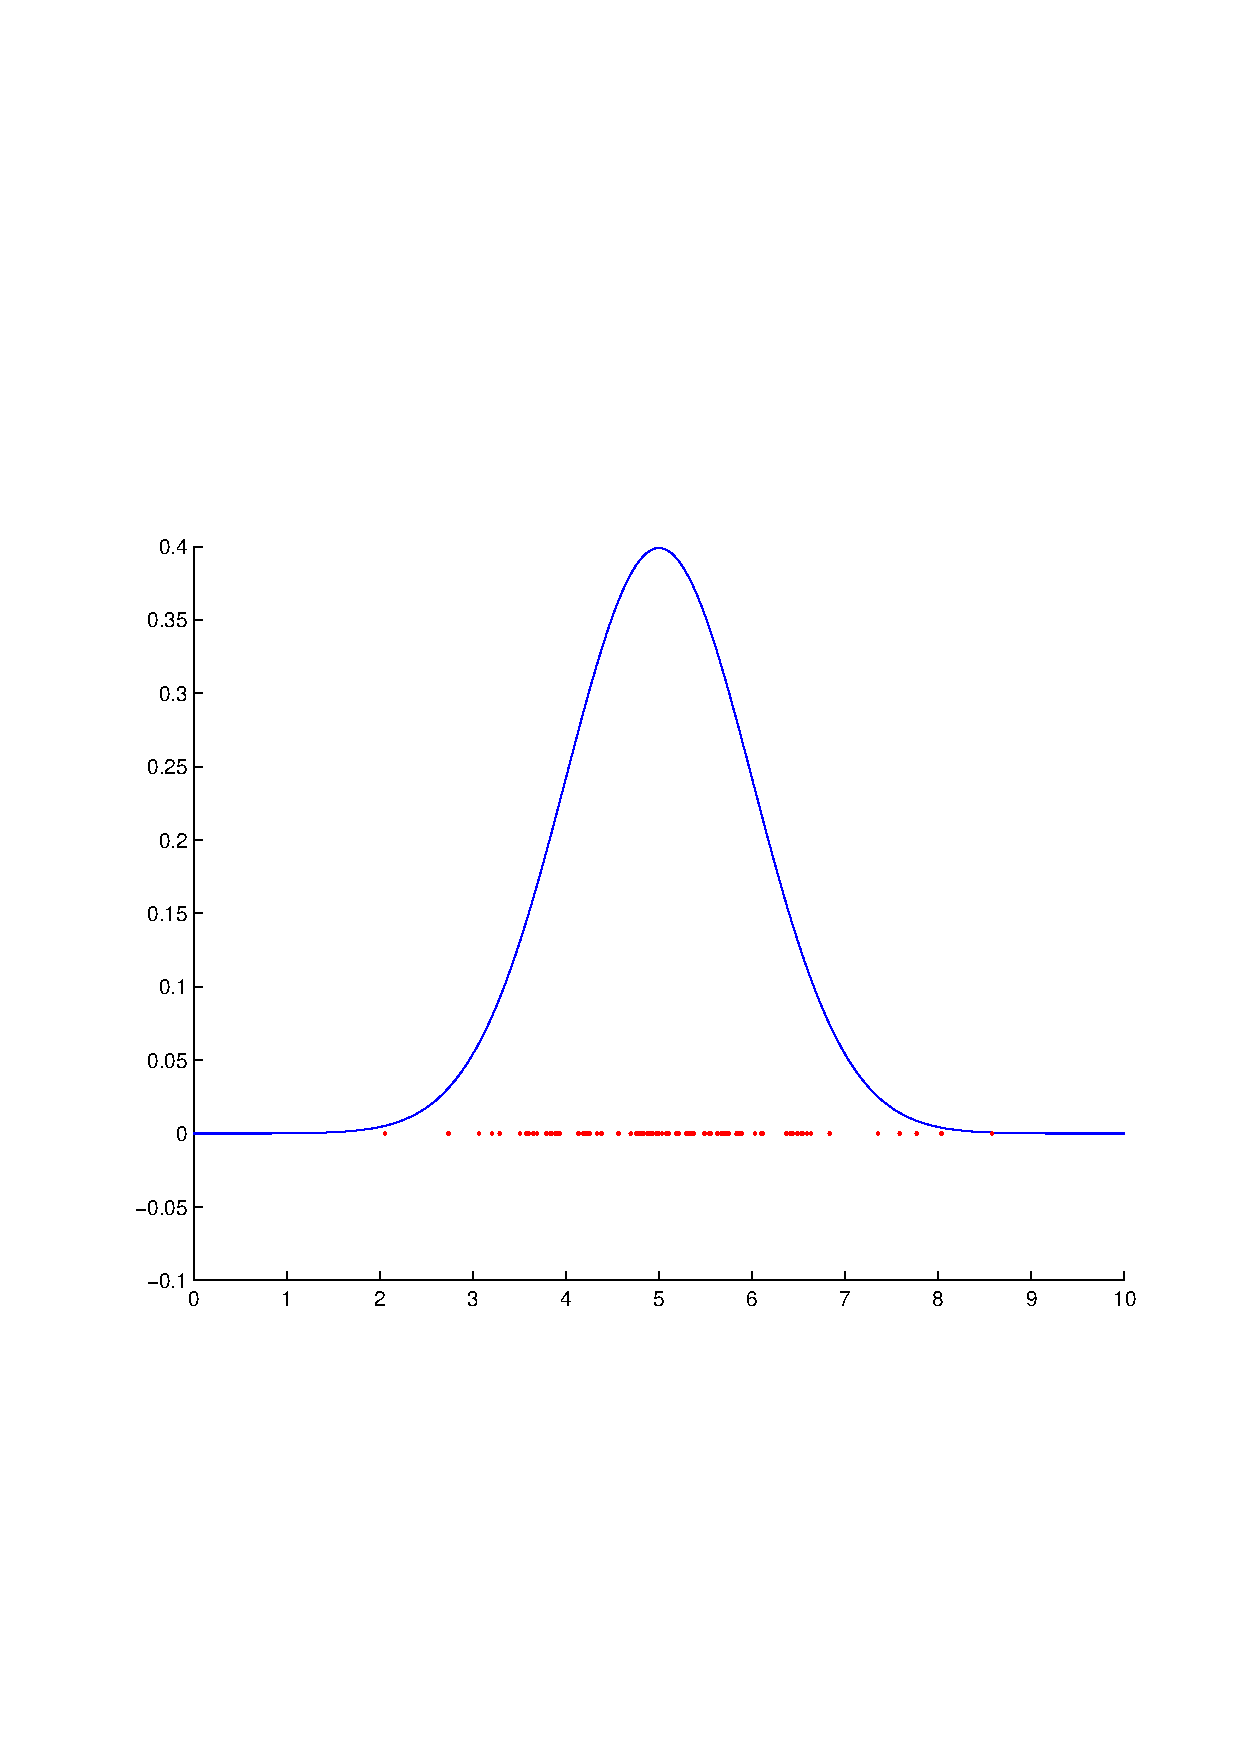
\includegraphics[width=0.7\columnwidth]{MonteCarlo.pdf}%
\caption{An analytic probability density (blue) may be approximated by a set of samples drawn from it (red)}%
\label{fig:MonteCarlo}%
\end{figure}

Often, it will not even be possible to sample from the desired distribution. We therefore use importance sampling (IS) or Markov chain Monte Carlo methods to generate these samples. The principle of a particle filter is that we recursively generate such a set of particles to approximate $P(X_{1:t}|Y_{1:t})$ given a previous set representing $P(X_{1:t-1}|Y_{1:t-1})$.

\subsection{The basics}

With a PF, we approximate a probability distribution with a set of (weighted) samples drawn from that distribution.

\begin{equation}
P(X) \approx \frac{1}{N} \sum_m{W^{(m)} \delta_{X^{(m)}} (X)}
\label{eq:ParticleApprox}
\end{equation}

where $\delta (x)$ represents a unit probability point mass at a point $x$, and $\sum_m{W^{(m)}}=1$. Such a method allows us to represent any probability distribution of arbitrary complexity, including multidimensional, multimodal, mixed distributions. As the number of particles increases, the accuracy of the approximation improves at the expense of computational complexity. Thus we have the required tool for estimation in non-linear, non-Gaussian scenarios.

We still face the problem of how to generate these samples. The conventional method for this is Sequential Importance Sampling with Resampling (SISR). For a more complete and traditional introduction to this method, see \cite{Cappe2007} or \cite{Doucet2009}. Here we follow an outline similar to that used for the derivation of the auxiliary particle filter of \cite{Pitt1999}.

Suppose we have a particle approximation to the joint posterior distribution from the previous frame, $\hat{P}(X_{1:t-1}|Y_{1:t-1})$. Each particle represents a path through time, $X_{1:t-1}^{(m)}$, and has an associated weight, $W_{t-1}^{(m)}$. Let us suppose also that the unweighted particles may be considered samples from another distribution:

\begin{equation}
\mu(X_{1:t-1}|Y_{1:t-1}) \approx \frac{1}{N} \sum_m{W^{(m)} \delta_{X_{1:t}^{(m)}} (X_{1:t})}
\label{eq:UnweightParticleDistn}
\end{equation}

Thus for a given particle,

\begin{equation}
\hat{P}(X_{1:t-1}^{(m)}|Y_{1:t-1}) = W_t^{(m)} \mu(X_{1:t-1}^{(m)}|Y_{1:t-1})
\label{eq:}
\end{equation}

We would like to generate a new particle set which includes the current time instance. We propose a new set of extended tracks from a factored proposal distribution $X_{1:t} \sim q(X_{1:t}|Y_{1:t}) = q(X_{t}|Y_{t}, X_{1:t-1}) q(X_{1:t-1}|Y_{1:t})$. The two factors are the proposal probabilities for the new state value, $X_t$ and the history, $X_{1:t-1}$, respectively. Particles are then weighted to take account of the difference between the targeted posterior distribution and the importance distribution:

\begin{equation}
W_t^{(m)} = \frac{P(X_{1:t}^{(m)}|Y_{1:t})}{q(X_{1:t}^{(m)}|Y_{1:t})}
\label{eq:ImportanceWeights}
\end{equation}

The simplest choice for the history proposal is $q(X_{1:t-1}|Y_{1:t}) = \mu(X_{1:t-1}|Y_{1:t-1})$, which can be implemented by simply keeping the same set of paths as the previous particle set. This is equivalent to an ordinary IS step with no resampling, and importance weights are given by:

\begin{equation}
W_t^{(m)} = \frac{P(X_{1:t}^{(m)}|Y_{1:t})}{q(X_{1:t}^{(m)}|Y_{1:t})}
\approx \frac{W_{t-1}^{(m)}P(X_{1:t}^{(m)}|Y_{1:t})}{P(X_{1:t-1}^{(m)}|Y_{1:t-1}) q(X_{t}^{(m)}|X_{t-1}^{(m)}, Y_{t})}
\propto \frac{W_{t-1}^{(m)} P(Y_t|X_t^{(m)})P(X_t^{(m)}|X_{t-1}^{(m)})}{q(X_t^{(m)}|X_{t-1}^{(m)}, Y_t)}
\label{eq:NoResampIW}
\end{equation}

Alternatively, we could use $q(X_{1:t-1}|Y_{1:t}) = \hat{P}(X_{1:t-1}|Y_{1:t-1})$ as the history proposal, i.e. sample from the weighted particle distribution which approximates the previous posterior. This is equivalent to an IS step preceeded by resampling. Importance weights are now given by:

\begin{equation}
W_t^{(m)} = \frac{P(X_{1:t}^{(m)}|Y_{1:t})}{q(X_{1:t}^{(m)}|Y_{1:t})}
\approx \frac{P(X_{1:t}^{(m)}|Y_{1:t})}{P(X_{1:t-1}^{(m)}|Y_{1:t-1}) q(X_{t}^{(m)}|X_{t-1}^{(m)}, Y_{t})}
\propto \frac{ P(Y_t|X_t^{(m)})P(X_t^{(m)}|X_{t-1}^{(m)})}{q(X_t^{(m)}|X_{t-1}^{(m)}, Y_t)}
\label{eq:WithResampIW}
\end{equation}


\subsection{Auxiliary sampling}

We can generalise the form of our history proposal distribution by weighting the particles from the previous posterior distribution with any arbitrary set of weights.

\begin{equation}
q(X_{1:t-1}|Y_{1:t}) = \frac{1}{N} \sum_m {V_t^{(m)} \delta_{X} (x_{1:t}^{(m)})}
\label{eq:AuxiliarySamplingProposal}
\end{equation}

Now we have

\begin{equation}
\hat{P}(X_{1:t-1}^{(m)}|Y_{1:t-1}) = \frac{W_{t-1}^{(m)}}{V_t^{(m)}} q(X_{1:t-1}^{(m)}|Y_{1:t})
\label{eq:}
\end{equation}

giving a general form for the importance weights

\begin{multline}
W_t^{(m)} = \frac{P(X_{1:t}^{(m)}|Y_{1:t})}{q(X_{1:t}^{(m)}|Y_{1:t})}
\approx \frac{W_{t-1}^{(m)}}{V_{t}^{(m)}} \times \frac{P(X_{1:t}^{(m)}|Y_{1:t})}{P(X_{1:t-1}^{(m)}|Y_{1:t-1}) q(X_{t}^{(m)}|X_{t-1}^{(m)}, Y_{t})}\\
\propto \frac{W_{t-1}^{(m)}}{V_{t}^{(m)}} \times \frac{ P(Y_t|X_t^{(m)})P(X_t^{(m)}|X_{t-1}^{(m)})}{q(X_t^{(m)}|X_{t-1}^{(m)}, Y_t)}
\label{eq:AuxiliaryIW}
\end{multline}

A suitable choice for the auxiliary proposal weights is the predictive likelihood of the next measurement, i.e.

\begin{equation}
V_t^{(m)} = P(Y_t|X_{t-1}^{(m)})
\label{eq:}
\end{equation}

This favours the selection of particles which better explain the new observation. This quantity is often not easily calculable, so approximations may be used, for example using a Gaussian approximation.



\subsection{Degeneracy and resampling}
The simplest history proposal is given by $q(X_{1:t-1}|Y_{1:t}) = \mu(X_{1:t-1}|Y_{1:t-1})$. This may be `sampled' by simply keeping the $N$ particles from the previous processing step, which is thus equivalent to importance sampling with no resampling. Multiple steps of this nature will lead to a fall in particle diversity, as many of the weights tend towards 0. This occurs because of the recursive nature of the importance weight calculation in equation~\ref{eq:NoResamIW}. The solution to this degeneracy is to use the other form of history proposal, $q(X_{1:t-1}|Y_{1:t}) = \hat{P}(X_{1:t-1}|Y_{1:t-1})$, equivalent to importance sampling with resampling. Such a proposal will require additional computation time, but the weight updates are no longer recursive, see equation~\ref{eq:ResamIW}, so diversity is improved.

The resampling/history-sampling may be conducted in a variety of ways. The simplest is multinomial sampling, in which each particle is sampled independently with replacement. In residual sampling, particles are sampled from the particle distribution without replacement, i.e. after a particle is selected, the probability of selecting it again is reduced. Finally, for systematic resampling, a finite real line is divided into sections corresponding to the weight of each particle. Particles are sampled by choosing regular points along this line, with some constant, random offset. The final method produces the least variance in the number of child particles chosen from each parent given the weights, and thus introduces the least Monte Carlo error. For more details see \cite{Doucet2009} and the references therein.

Degeneracy is measured using the Effective Sample Size of \cite{Liu1995}, which is given by:

\begin{equation}
ESS = \frac{1}{N} \sum_m W^{(m)2}
\label{eq:ESS}
\end{equation}

where $W^{(m)}$ are the particle weights, and there are $N$ particles. If ESS falls below some chosen threshold, resampling this required to replenish particle diversity.



\subsection{Importance distributions}

It remains to choose the the importance distribution for the current state, $q(X_{t}|X_{t-1}, Y_{t})$. In the original ``bootstrap filter'' of \cite{Gordon1993}, this was set equal to the transition density, $P(X_t|X_{t-1})$, which leads to cancellation in the expression for importance weights. This is simple but not necessarily optimal. For example if the process noise is high, the samples of $X_t$ will be widely spread. If, however, the observation noise is comparitively low, many or most of the samples will be far from the observation and will have a low weight, giving us poor particle diversity.

An improved choice of proposal distribution is given by:

\begin{equation}
q(X_{t}|X_{t-1}, Y_{t}) = P(X_t|X_{t-1}, Y_t) = \frac{P(Y_t|X_t)P(X_t|X_{t-1})}{P(Y_t|X_{t-1})}
\label{eq:OptimalImportanceDist}
\end{equation}

This is often known as the ``optimal importance distribution''. The importance weights for a step without resampling are now given by:

\begin{equation}
W_t^{(m)} \propto \frac{ W_{t-1}^{(m)} }{ V_t^{(m)} } \times \frac{ P(Y_t|X_t^{(m)})P(X_t^{(m)}|X_{t-1}^{(m)}) }{q(X_t^{(m)}|X_{t-1}^{(m)}, Y_t)} \propto \frac{ W_{t-1}^{(m)} }{ V_t^{(m)} } \times P(Y_t|X_{t-1}^{(m)})
\label{eq:OptimalImportanceWeights}
\end{equation}

If the auxiliary weights are set to $V_t^{(m)}=P(Y_t|X_{t-1}^{(m)})$ then all weights are equal throughout, and resampling will never be required. In general, the optimal importance distribution will not be samplable, but proposals using Gaussian approximations of this form may be used.
\section{MCMC in da house - Markov chains for particle filtering}
The previous sections have focussed on the traditional, SISR particle filter. Here we examine the MCMC version. The mathematical extensions required are minimal.

MCMC methods allow us to generate an unweighted particle approximation to a target probability distribution. Particles are generated sequentially, each dependent on the last, giving us a Markov chain whose stationary distribution is equal to that which we wish to approximate. For a basic MH step, a proposal distribution is sampled to acquire a new candidate state. With some probability this candidate is accepted as the new state. Otherwise, it is rejected and the old state is kept as the new state. The acceptance probability required to make $P(X)$ the stationary distribution of the Markov chain is given by

\begin{equation}
\alpha = \min \bigg ( 1,  \frac{ P(X_{\text{new}}) q(X_{\text{old}}|X_{\text{new}}) }{ P(X_{\text{old}}) q(X_{\text{new}}|X_{\text{old}}) }  \bigg ).
\label{eq:MHAcceptance}
\end{equation}

This will be appear familiar as the ratio of the importance weights the old and candidate states would receive in a SISR scheme. In a MCMC particle filtering scheme we target the usual joint posterior distribution

\begin{equation}
P(X_{1:t}|Y_{1:t}) = \frac{P(Y_t|X_t)P(X_t|X_{t-1})P(X_{1:t-1}|Y_{1:t-1})}{P(Y_t|Y_{1:t-1})}.
\label{eq:MCMCPFTarget}
\end{equation}

As for the SISR particle filter, the proposal distribution factorises as  $X_{1:t} \sim q(X_{1:t}|Y_{1:t}) = q(X_{t}|Y_{t}, X_{1:t-1}) q(X_{1:t-1}|Y_{1:t})$. We can use a biased history proposal in the flavour of the auxiliary particle filter, as in equation~\ref{eq:AuxiliarySamplingProposal}.

We now adopt the following notation: $X$ for the new state of the Markov chain, and $Z$ for the old state, with $V_{X,t}$ and $V_{Z,t}$ respectively for the auxiliary proposal weights. Using these expansions, the acceptance probability is given by

\begin{IEEEeqnarray}{rCl}
\alpha & = & \min \bigg ( 1,  \frac{ P(X_{1:t}|Y_{1:t}) q(Z_{1:t}|Y_{1:t} }{ P(Z_{1:t}|Y_{1:t}) q(X_{1:t}|Y_{1:t} }  \bigg ) \nonumber \\
 & = & \min \bigg ( 1,  \frac{ P(Y_t|X_t)P(X_t|X_{t-1}) q(Z_t|Y_t, Z_{1:t-1}) V_{Z,t} }{ P(Y_t|Z_t)P(Z_t|Z_{t-1}) q(X_t|Y_t, X_{1:t-1}) V_{X,t} }  \bigg ).
\label{eq:MCMCPFAcceptance}
\end{IEEEeqnarray}

The advantage of using a MCMC scheme is that we can vary only some subset of the state variables in each move if we choose. For example, we can have one sort of MH move which keeps the history the same, $X_{1:t}=Z_{1:t}$. This leads to a simplification of the equation for $\alpha$ and an improved probability of acceptance.


\chapter{The tracking model}
In this chapter we introduce the mathematical model for the object tracking problem which will be used throughout the rest of this report.

We first assume that our targets exist at singular points in space, and that targets move independently of each other. Each target will have be characterised by a state vector $x_{j,t}$. This state is composed of continuous-valued coordinates and evolves according to a hidden Markov model (HMM). At first, we will also assume that we know how many targets are in the scene and their starting locations, $x_{j,0}$.

\begin{equation}
x_{j,t} = f(x_{j,t-1}, v_{j,t})
\end{equation}

where $v_{j,t}$ is a random vector.

The targets are observed by a sensor which detects each with a probability $P_D$. If detected, the sensor returns a point observation at a location $y_t^{(i)}$ given by:

\begin{equation}
y_t^{(i)} = g(x_{j,t}, w_{j,t})
\end{equation}

where $w_{j,t}$ is another random vector, independent of $v_{j,t}$.

In addition to the target-originating observations, the sensor also detects a number of false alarms. We assume that these are generated by a Poisson process, with a uniform intensity over the observation area. The expected number of clutter observations in a frame is denoted $\mu_C$.

We denote the set of targets present as $X_t = \{x_{1,t}, x_{2,t}, ... , x_{K_t, t} \}$, and the set of observations as $Y_t = \{y_t^{(1)}, y_t^{(2)}, ... , y_t^{(M_t)} \}$.

We introduce an association variable for each target, $\lambda_{j,t}$, which indicates which of the observations in that frame was generated by this target, as shown in figure~\ref{fig:BasicTrackingAssoc}. If the target is not detected, then $\lambda_{j,t}$ is set to 0. We denote the set $\Lambda_t = \{\lambda_{1,t}, \lambda_{2,t}, ... , \lambda_{K_t, t} \}$. As each observation is generated by one target or clutter, no two elements of $\Lambda_t$ may take the same value, unless 0. (This is the constraint that the PMHT and PDAF relax.)

\begin{figure} \centering
\input{BasicTrackingAssoc.pdf_tex}%
\caption{A simple two-target tracking problem illustrating the different possible associations at one time step. Hidden states shown as blue crosses. Observations shown as red circles.}
\label{fig:BasicTrackingAssoc}%
\end{figure}

The graphical model including the association variables is shown in figure~\ref{fig:HMMAssoc}.

\begin{figure}%
\centering

\tikzstyle{state} = [circle,thick,minimum size=1.2cm,draw=black]
\tikzstyle{assoc} = [circle,thick,minimum size=1.2cm,draw=blue]
\tikzstyle{observ} = [circle,thick,minimum size=1.2cm,draw=red]

\begin{tikzpicture}[>=latex,text height=1.5ex,text depth=0.25ex]

	\matrix[row sep=0.5cm,column sep=0.5cm] {
		&
		\node (y_k-1) [observ]{$Y_{k-1}$}; &
		&
		\node (y_k) [observ]{$Y_{k}$}; &
		&
		\node (y_k+1) [observ]{$Y_{k+1}$}; &
		& \\
		& &
		\node (l_k-1) [assoc]{$\Lambda_{k-1}$}; &
		&
		\node (l_k) [assoc]{$\Lambda_{k}$}; &
		&
		\node (l_k+1) [assoc]{$\Lambda_{k+1}$}; & \\
		\node (x_k-2) {$\cdots$}; &
		\node (x_k-1) [state]{$X_{k-1}$}; &
		&
		\node (x_k) [state]{$X_{k}$}; &
		&
		\node (x_k+1) [state]{$X_{k+1}$}; &
		&
		\node (x_k+2) {$\cdots$}; \\
	};

	\path[->]
		(x_k-2) edge[thick] (x_k-1)
		(x_k-1) edge[thick] (x_k)
		(x_k) edge[thick] (x_k+1)
		(x_k+1) edge[thick] (x_k+2)
		
		(x_k-1) edge[thick] (y_k-1)
		(x_k) edge[thick] (y_k)
		(x_k+1) edge[thick] (y_k+1)
		
		(l_k-1) edge[thick] (y_k-1)
		(l_k) edge[thick] (y_k)
		(l_k+1) edge[thick] (y_k+1)
		;

\end{tikzpicture}
\caption{Graphical model for tracking including association variables.}%
\label{fig:HMMAssoc}%
\end{figure}

If we wished to calculate the posterior distribution over the target states, $X_t$, we would need to marginalise the association variables in the calculation of the likelihood term:

\begin{equation}
P(Y_t|X_t) = \sum_{\Lambda_t} P(\Lambda_t) \prod_{j=1}^{K_t} P(y_t^{(\lambda_{j,t})}|x_{j,t})
\label{eq:MarginaliseAssociations}
\end{equation}

where the summation is over all feasible values of $\Lambda_t$. The number of terms in this summation combinatorially in the number of targets and the number of observations, and may be prohibitively large if there are many targets or observations in the scene. If it is necessary to calculate the likelihood very often, as in a particle filter, it may be preferable to estimate $\Lambda_t$ instead of marginalising it. The target distribution is now:

\begin{equation}
P(X_{1:t}, \Lambda_{1:t}|Y_{1:t}) = \frac{P(Y_t|X_t, \Lambda_t) P(X_t|X_{t-1}) P(\Lambda_t) P(X_{1:t-1}, \Lambda_{1:t-1}|Y_{1:t-1})}{P(Y_t|Y_{1:t-1})}
\label{eq:MTPosterior}
\end{equation}

We now consider the terms of this equation one at a time.

\section{Observation Likelihood}
The likelihood given the associations is given by:

\begin{equation}
P(Y_t|X_t, \Lambda_t) = V^{-(M_t-M_{T,t})} \prod_{\lambda_{j,t} \ne 0} P(y_t^{(\lambda_{j,t})}|x_{j,t})
\label{eq:MTLikelihood}
\end{equation}

where $V$ is the volume of the observation region, and thus $V^{-1}$ is the likelihood of a clutter obervation, and where $M_{T,t} = \left| \{ \lambda_{j,t} \ne 0 \} \right|$. This can be conveniently factorised as

\begin{equation}
P(Y_t|X_t, \Lambda_t) = V^{-(M_t-K_t)} \prod_{j=1}^{K_t} \begin{cases} P(y_t^{(\lambda_{j,t})}|x_{j,t}) & \lambda_{j,t} \ne 0 \\ V^{-1} & \lambda_{j,t} = 0 \end{cases}
\label{eq:MTFactorisedLikelihood}
\end{equation}

This expression contains a factor for each target, and a coefficient independent of the state. This coefficient will either cancel out (MCMC) or be discarded in the weight normalisation (SISR).



\section{Transition Dynamics}
Similarly, because of our independence assumption on the targets, the transition dynamic term will factorise:

\begin{equation}
P(X_t|X_{t-1}) = \prod_{j=1}^{K_t} P(x_{j,t}|x_{j-1})
\label{eq:MTFactorisedTransition}
\end{equation}



\section{Association Likelihood}
The association variable, $\lambda_t$, tells us how many targets have been detected (and how many have not), and how many clutter observations are present. To construct a prior distribution on this, consider the $\lambda_{j,t}$s in turn. Each one can be either 0 with probability $(1-P_D)$, or an observation index with probability $P_D$. If it is the latter, there are $M_t - M_{\textnormal{taken}}$ indexes from which to choose, where $M_{\textnormal{taken}}$ is the number of observations already assigned to a previous target. Once we have considered all the targets, $M_{T,t}$ observations will have been assigned to targets, and all those remaining must be generated by the clutter process. The number of these is Poisson distributed. The association prior for feasible is $\Lambda_t$ thus given by:

\begin{multline}
P(\Lambda_t) = \underbrace{\frac{P_D^{M_t}}{M_t(M_t-1)...(M_t-M_{T,t})}}_\textnormal{detected targets} \underbrace{(1-P_D)^{(K-M_t)}}_\textnormal{undetected targets} \underbrace{\frac{\exp(-\mu_C) \mu_C^{(M_t-M_{T,t})}}{(M_t-M_{T,t})!}}_\textnormal{clutter} \\
= \frac{ \exp(-\mu_C) \mu_C^{(M_t-M_{T,t})} P_D^{M_t} (1-P_D)^{(1-M_t)} }{ M_t! }
\label{eq:MTAssociationLikelihood}
\end{multline}

while for invalid $\Lambda_t$ ($\lambda_{i,t}=\lambda_{j,t}$ for $i \ne j$, $\lambda_{i,t},\lambda_{j,t} \ne 0$), the probability is zero. Again, we can factorise this expression over the targets.

\begin{equation}
P(\lambda_t) = \frac{\exp(-\mu_C) \mu_C^{(M_t-K_t)}}{M_t!} \prod_{j=1}^{K_t} \begin{cases} P_D & \lambda_{j,t} \ne 0, \lambda_{j,t} \notin \{ \lambda_{1:j-1,t} \} \\ 0 & \lambda_{j,t} \in \{ \lambda_{1:j-1,t} \} \\ (1-P_D) \mu_C & \lambda_{j,t}=0 \end{cases}
\label{eq:MTFactorisedAssociationLikelihood}
\end{equation}

Just as for the observation likelihood, this expression has a factor for each target and a state-independent coefficient which can be ommitted for either a SISR or MCMC particle filter.



\section{Assumptions}
Here we summarise the assumptions made in the model formulations:

\begin{itemize}
	\item Targets and observations occur at singular points.
	\item The number of targets is known.
	\item Target starting locations known.
	\item Target states evolve independently of each other according to a HMM.
	\item Targets are detected in each frame with an independent probability $P_D$. A detected target generates one observation.
	\item A single target is associated with each observation.
	\item Clutter observations are generated by a homogeneous spatial Poisson process.
\end{itemize}



\section{Specific models}

\subsection{State transitions}
In this work we employ a Near-Constant Velocity (NCV) model. We omit the target index $j$ in the following and consider only a single spatial dimension. The extension to multiple dimensions is trivial. A target state, $x$, is written as a vector:

\begin{equation}
x = \begin{pmatrix}
	s \\ \dot{s}
\end{pmatrix}
\label{eq:}
\end{equation}

We define the target motion by a simple stochastic differential equation, in which acceleration is a Wiener process.

\begin{IEEEeqnarray}{rCl}
d\dot{s}_{\tau} & = & \sigma dW_{\tau} \\
ds_{\tau} & = & \dot{s}_{\tau}
\end{IEEEeqnarray}

Integrating these gives us

\begin{IEEEeqnarray}{rCl}
\dot{s}_{\tau} & = \dot{s}_0& + \sigma W_{\tau} \\
s_{\tau} & = & s_0 + \dot{s}_0 {\tau} + \sigma \int_0^{\tau} W_s ds
\end{IEEEeqnarray}

which we can rewrite in matrix form

\begin{equation}
\begin{bmatrix}s_{\tau} \\ \dot{s}_{\tau}\end{bmatrix} = \begin{bmatrix}1 & {\tau} \\ 0 & 1\end{bmatrix} \begin{bmatrix}s_0 \\ \dot{s}_0\end{bmatrix} + \sigma \begin{bmatrix}W_{\tau} \\ \int_0^{\tau} W_s ds \end{bmatrix}
\end{equation}

It is thus clear that the $x_{\tau}|x_0$ is normally distributed with mean $x_0$ and covariance 

\begin{equation}
\mathbb{V}[x_{\tau}] = \sigma^2 \mathbb{E}\begin{bmatrix}W_{\tau}^2 & W_{\tau} \int_0^{\tau} W_s ds \\ W_{\tau} \int_0^{\tau} W_s ds & \left( \int_0^{\tau} W_s ds \right)^2\end{bmatrix} = \sigma^2 \begin{bmatrix} {\tau} & \frac{{\tau}^2}{2} \\ \frac{{\tau}^2}{2} & \frac{{\tau}^3}{3}\end{bmatrix}
\end{equation}

The model can now be discretised onto a set of time point, indexed with $t$. The transition density is linear-Gaussian given by:

\begin{equation}
P(x_{t+1}|x_{t}) = \mathcal{N}(x_{t+1}|A x_{t},Q)
\label{eq:}
\end{equation}

Throughout this report, we will consider models in two spatial dimensions. Thus the matrices $A$ and $Q$ are given by:

\begin{equation}
A = \begin{bmatrix}
1 & 0 & P & 0 \\
0 & 1 & 0 & P \\
0 & 0 & 1 & 0 \\
0 & 0 & 0 & 1
\end{bmatrix}
\label{eq:}
\end{equation}

\begin{equation}
Q = \sigma^2 \begin{bmatrix}
P & 0 & \frac{P^2}{2} & 0 \\
0 & P & 0 & \frac{P^2}{2} \\
\frac{P^2}{2} & 0 & \frac{P^3}{3} & 0 \\
0 & \frac{P^2}{2} & 0 & \frac{P^3}{3} \\
\end{bmatrix}
\label{eq:}
\end{equation}

and $P$ is the sampling period.

\subsection{Observations}
We will use two different observation models. Firstly, linear-Gaussian where the position is observed directly:

\begin{equation}
P(y_t^{\lambda_t}|x_t) = \mathcal{N}(y_t^{\lambda_t}|C x_t, R)
\label{eq:}
\end{equation}

where $C$ is:

\begin{equation}
\begin{bmatrix}
1 & 0 & 0 & 0 \\
0 & 1 & 0 & 0 \\
\end{bmatrix}
\label{eq:}
\end{equation}

Secondly, we consider a polar observation model, of the form used for radar systems.

\begin{equation}
P(y_t^{\lambda_t}|x_t) = \mathcal{N}(y_t^{\lambda_t}|h(x_t), R)
\label{eq:}
\end{equation}

where

\begin{equation}
h(x_t) = \begin{bmatrix}
\arctan \left( \frac{x_{2,t}}{x_{1,t}} \right)\\
\sqrt{ (x_{1,t}^2 + (x_{2,t}^2 }
\end{bmatrix}
\label{eq:}
\end{equation}

We will need a linearised, EKF approximation of this model for use in proposal distributions. This will require the jacobian of the observation function:

\begin{equation}
C_t = \begin{bmatrix} \frac{\partial h_1}{\partial x_{1,t}} & \frac{\partial h_1}{\partial x_{2,t}} & \frac{\partial h_1}{\partial \dot{x}_{1,t}} & \frac{\partial h_1}{\partial \dot{x}_{2,t}} \\ \frac{\partial h_2}{\partial x_{1,t}} & \frac{\partial h_2}{\partial x_{2,t}} & \frac{\partial h_2}{\partial \dot{x}_{1,t}} & \frac{\partial h_2}{\partial \dot{x}_{2,t}} \end{bmatrix}
= \begin{bmatrix} \frac{-x_{2,t}}{x_{1,t}^2 + x_{2,t}^2} & \frac{x_{1,t}}{x_{1,t}^2 + x_{2,t}^2} & 0 & 0 \\ \frac{x_{1,t}}{\sqrt{x_{1,t}^2 + x_{2,t}^2}} & \frac{x_{2,t}}{\sqrt{x_{1,t}^2 + x_{2,t}^2}} & 0 & 0 \end{bmatrix}
\label{eq:}
\end{equation}

The effect of such an approximation is shown in figure~\ref{fig:EKFradar}

\begin{figure}[!hbt] \centering
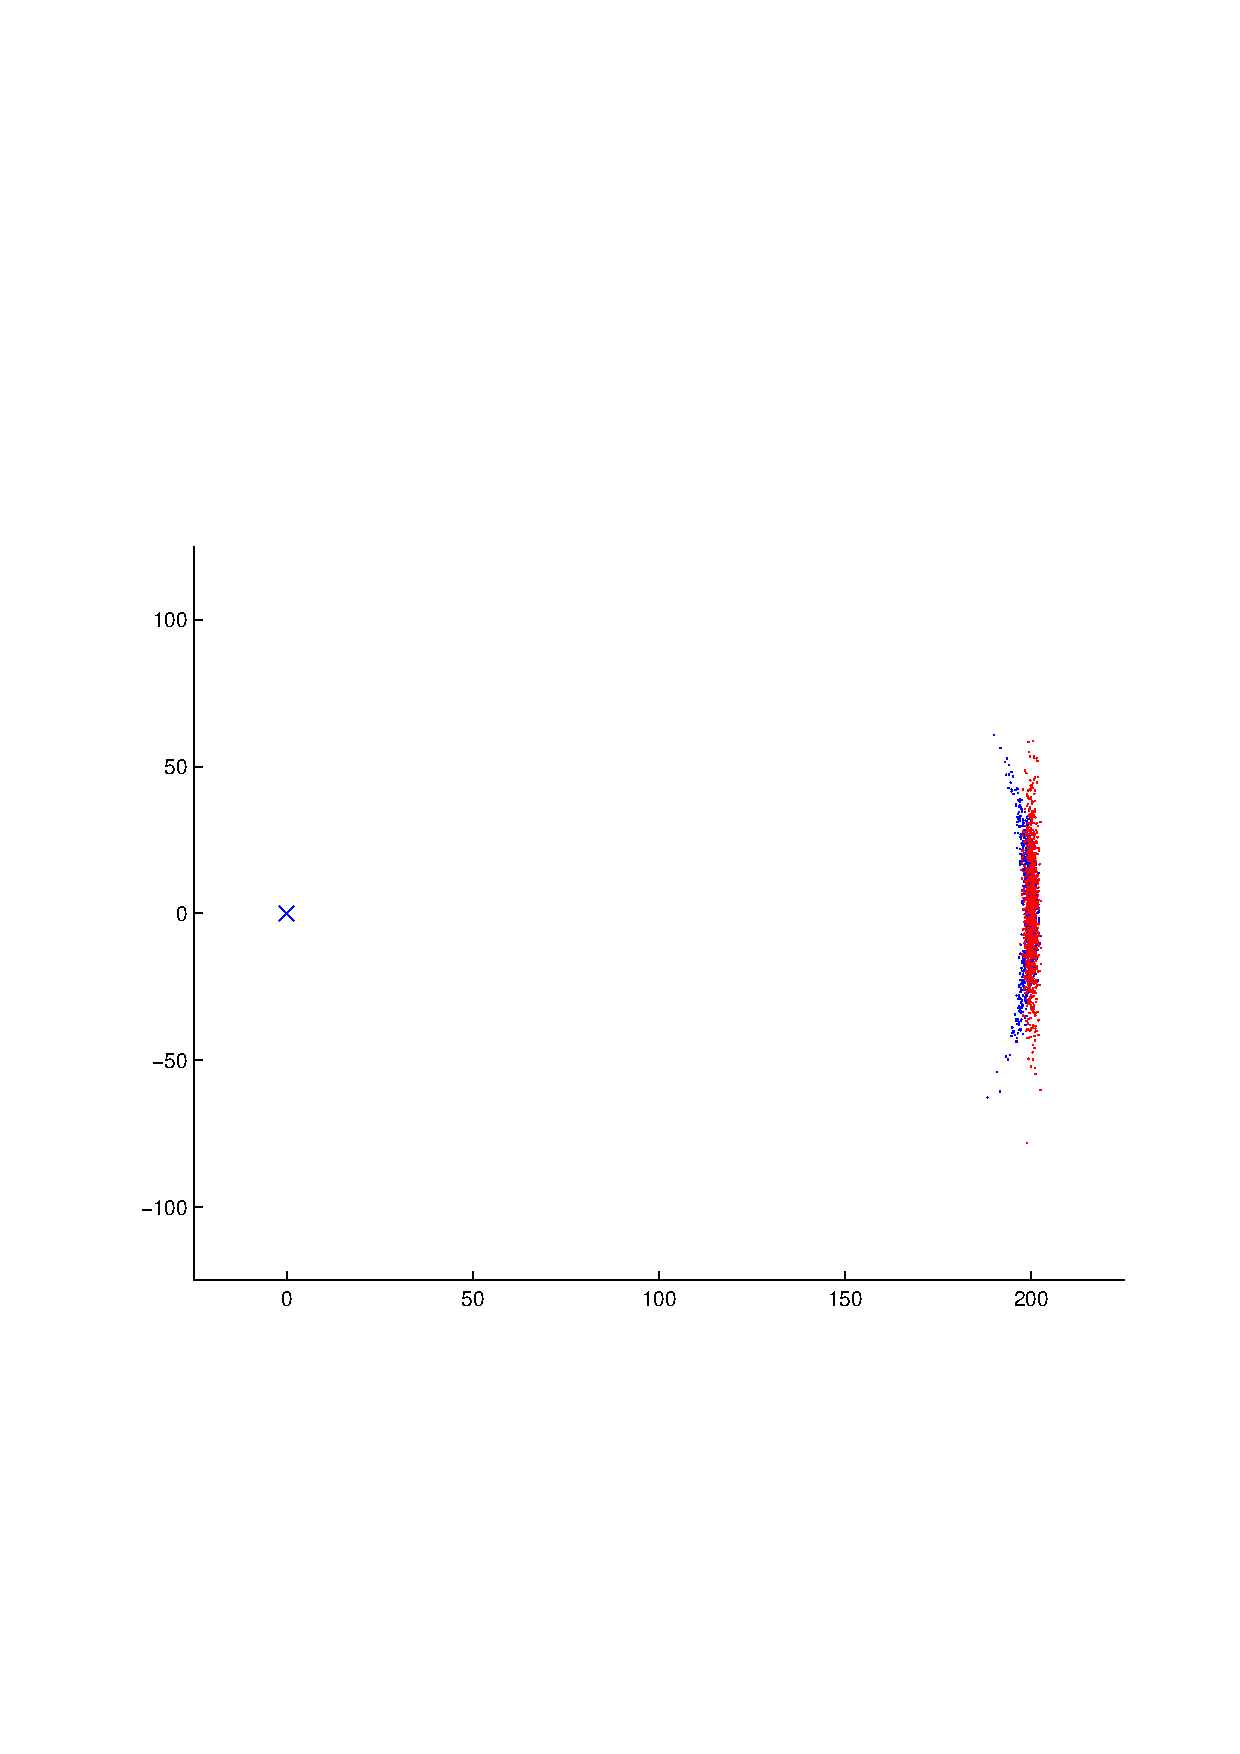
\includegraphics[width=0.7\columnwidth]{EKF.pdf}%
\caption{Samples from the nonlinear observation distribution (blue) and from the EKF approximation (red).}%
\label{fig:EKFradar}%
\end{figure}

\chapter{Fixed Lag Estimation for Tracking}\label{FixedLag}
\section{The benefits of delaying}
A basic filter, the Kalman filter included, allows us to estimate the latest value of a hidden state given all previous observations. However, if we wait until the next observation arrives, we can often make a much better estimate - we now know where the state is going as well as where it came from. This is the idea exploited by the Kalman smoother. In fact, as we have seen, the regular particle filter gives us an estimate of the entire state history, $X_{1:t}$. However, due to the resampling process, the particle diversity of the state distribution for previous frames falls as we move further back in time.

As well as giving poor estimates for state distributions, a further disadvantage of this falling diversity in a tracking context is a tendency to lose tracks. Suppose that in some frame the majority of particles associate with a particular likely-looking observation and head off in one direction, but that a few frames later it becomes apparent that this is an error, and that the correct route goes another way. With an ordinary SISR particle filter the majority of the particles are now eliminated by resampling. The particle diversity of the state estimate will be very poor, and in a challenging problem there is a good chance that the track will be lost.

PICTURE

Improved estimates for previous state distributions can be made using the resample-move (RM) method of \cite{Gilks2001} to rejeuvenate the particle diversity. However, this requires running at least one MH move for each particle on top of the usual importance sampling step, which will be computationally expensive. Furthermore, the RM steps will cause most rejeuvenation in the most recent frames, which will be discarded in the next frame.

An alternative framework for fixed lag estimation is presented by \cite{Doucet2006}. Now we propose new values not only for the current state but also the previous states within some time window. The effect of this in our tracking example is that we can `redirect' particles which have gone astray along the correct path, maintaining a better particle diversity and reducing the probability of track loss. \cite{Doucet2006} report that RM does not perform as well as their fixed-lag estimation method, although the two shemes are related.
\section{A mathematical framework for fixed lag estimation}
Here we consider the mathematical framework for fixed-lag estimatation, as presented by \cite{Doucet2006} and \cite{Briers2006}.

As before, the target posterior distribution in which we are interested is the familiar $P(X_{1:t}|Y_{1:t})$. However, the proposal mechanism now becomes more complex, because we will be replacing states in an existing particle. We first propose a particle from which to take the state ``history'', that is $X_{1:t-L}$. However, if we take this from the particle distribution from the previous step we get more of the path than we need, because each particle is a set of states $X_{1:t-1}$. The final $L-1$ states will be replaced when by a new ``present'', $X'_{t-L+1:t}$, drawn from an importance distribution. The complete proposal is thus

\begin{equation}
\{X_{1:t-L}, X'_{t-L+1:t}\} \sim \int q(X_{1:t-1}|Y_{1:t-1}) q(X'_{t-L+1}|X_{1:t-1}, Y_{t-L+1:t}) dX_{t-L+1:t-1}
\label{eq:DumbFLProposal1}
\end{equation}

where $q(X_{1:t-1}|Y_{1:t-1})$ is a proposal distribution using the arbitrarily-weighted particles from $\hat{P}(X_{1:t-1}|Y_{1:t-1})$, in the auxiliary sampling sense. This integral is required for calculation of importance weights of acceptance probabilities, but in general it will be intractable. If we were to restrict our proposals to depend only on the history, i.e. use $q(X_{t-L+1:t}|X_{1:t-L}, Y_{t-L+1:t})$, then the proposal would become

\begin{equation}
\{X_{1:t-L}, X'_{t-L+1:t}\} \sim \hat{P}(X_{1:t-L}|Y_{1:t-1}) q(X'_{t-L+1}|X_{1:t-1}, Y_{t-L+1:t})
\label{eq:DumbFLProposal2}
\end{equation}

However, with this proposal, in order to evaluate importance weights or acceptance probabilities we still need to calculate

\begin{equation}
P(X_{1:t-L}|Y_{1:t-1}) = \frac{P(Y_{t-L+1:t-1}|X_{t-L}^{(m)}) P(X_{1:t-L}|Y_{1:t-L} }{P(Y_{t-L+1:t-1}|Y_{1:t-L})}
\label{eq:}
\end{equation}

The problematic term is:

\begin{equation}
P(Y_{t-L+1:t}|X^{(m)}_{t-L}) = \int P(Y_{t-L+1:t}|X^{(m)}_{t-L}, X_{t-L+1:t}) P(X_{t-L+1:t}|X^{(m)}_{t-L}) dX_{t-L+1:t}
\label{eq:}
\end{equation}

This is intractable. The solution to this problem proposed in \cite{Doucet2006} is to augment the dimension of the target distribution to include the discarded tracks. The new target is:

\begin{equation}
P(X_{1:t-L}, X'_{t-L+1:t}|Y_{1:t}) \rho(X_{t-L+1:t-1}|X_{1:t-L}, X'_{t-L+1:t})
\label{eq:}
\end{equation}

Once a particle approximation has been generated for this target the required posterior distribution may be obtained by marginalisation. As we are simply going to discard the old track sections $X_{t-L+1:t-1}$, the choice of $\rho(.)$ does not alter the distribution of the posterior. However, the variance of weights/acceptance probabilities may be affected.

With an expanded space for the target distribution there is no need to marginalise the previous states. The proposal distribution now becomes:

\begin{equation}
\{X_{1:t-1}, X'_{t-L+1:t}\} \sim q(X_{1:t-1}|Y_{1:t-1}) q(X'_{t-L+1:t}|X_{1:t-1}, Y_{t-L+1:t})
\label{eq:ExtendedFLProposal}
\end{equation}

Histories are proposed from the $t-1$ frame in the normal manner, see equation~\ref{eq:AuxiliarySamplingProposal}.

\cite{Doucet2006} show that the optimum choice (in the minimal importance weight variance sense) of artifical conditional distribution is given by 

\begin{equation}
\rho(X_{t-L+1:t-1}|X_{1:t-L}, X'_{t-L+1:t}) = P(X_{t-L+1:t-1}|X_{t-L}, Y_{t-L+1:t-1})
\label{eq:}
\end{equation}

with the current proposal distribution set to

\begin{equation}
q(X'_{t-L+1:t}|X_{1:t-s}, Y_{t-L+1:t}) = P(X'_{t-L+1:t}|X_{t-L}, Y_{t-L+1:t})
\label{eq:}
\end{equation}

Thus both artificial conditional and proposal distribution should equal to the conditional posterior. This is neither samplable nor calculable. However, it is intuitive to use the same approximation for each by making the artificial conditional equal to the proposal. The ratio of target to proposal probability is then given by:

\begin{multline}
\frac{ P(X_{1:t-L}, X'_{t-L+1:t}|Y_{1:t}) \rho(X_{t-L+1:t-1}|X_{1:t-L}, X'_{t-L+1:t}) }{ q(X_{1:t-1}|Y_{1:t-1}) q(X'_{t-L+1:t}|X_{1:t-1}, Y_{t-L+1:t}) } \\
= \frac{W_t}{V_t} \frac{ P(X_{1:t-L}, X'_{t-L+1:t}|Y_{1:t}) q(X_{t-L+1:t-1}|X_{1:t-L}, X'_{t-L+1:t-2}, Y_{t-L+1:t-1}) }{ P(X_{1:t-1}|Y_{1:t-1}) q(X'_{t-L+1:t}|X_{1:t-1}, Y_{t-L+1:t}) } \\
\propto \frac{W_t}{V_t} \frac{ P(Y_{t-L+1:t}|X'_{t-L+1:t}) P(X'_{t-L+1:t}|X_{t-L}) q(X_{t-L+1:t-1}|X_{1:t-L}, X'_{t-L+1:t-2}, Y_{t-L+1:t-1}) }{ P(Y_{t-L+1:t-1}|X_{t-L+1:t-1}) P(X_{t-L+1:t-1}|X_{t-L}) q(X'_{t-L+1:t}|X_{1:t-1}, Y_{t-L+1:t}) }
\label{eq:}
\end{multline}

ARGH! NO! THE PROPOSAL CAN ALSO DEPEND ON $Z$ in the MCMC CASE!!!





\subsection{Proposing older histories}
CONSIDER MOVING THIS TO THE MCMC IMPLEMENTATION SECTION
So far we have chosen to propose histories from the $t-1$ particle distribution. However, a suitable history could be also selected from the $t-s$ distribution, for $1 \le s \le L$. In a situation where a track has not been detected for several consecutive frames, taking a history from further in the past may make the proposal of a good candidate more probable.

PICTURE

The history proposal lag variable $s$ can most easily be handled by sampling it too.

\begin{equation}
\{X_{1:t-s}, X'_{t-L+1:t}, s\} \sim q(s) q(X_{1:t-s}|Y_{1:t-s}) q(X'_{t-L+1:t}|X_{1:t-s}, Y_{t-L+1:t})
\label{eq:ExtendedFLProposal}
\end{equation}

This is simply equivalent to enlarging the pool of particles from which we propose histories. $q(s)$ is simply a modification to the particle proposal weights.

SOMETHING ABOUT CONSERVATIVE RESAMPLING AND ITS EQUIVALENT AIM
\label{sec:FixedLag2}
\section{Application to tracking}\label{FixedLag_App}
\subsection{Importance distributions}

The dimensionality of a fixed lag particle filter will generally be very large. Consider a problem where each target has a 4-dimensional kinematic state (postion and velocity in $x$ and $y$) and an observation-association index. This gives us five dimensions per target per time step. If we use a lag window with length $L=5$ and 5 targets we will have a 125 dimensional state. If we used a basic, bootstrap approach to such a problem, the chances of even a single particle following the correct path are negligible. Instead we must exploit the strong correlations between states arising from the structure of the problem. We first factorise the proposal over the targets:

\begin{equation}
q(X_{t-L+1:t}, \Lambda_{t-L+1:t}|X_{t-L}, Y_{t-L+1:t}) = \prod_{j=1}^{K_t} q(x_{j,t-L+1:t}, \lambda_{j,t-L+1:t}|\lambda_{1:j-1,t-L+1:t}, x_{j,t-L}, Y_{t-L+1:t})
\label{eq:}
\end{equation}

Thus, the targets may be proposed sequentially. The proposal for each target is then further decomposed.

\begin{IEEEeqnarray}{rCl}
q(x_{j,t-L+1:t}, \lambda_{j,t-L+1:t}|\lambda_{1:j-1,t-L+1:t}, x_{j,t-L}, Y_{t-L+1:t}) & & \nonumber \\
 & = & q(\lambda_{j,t-L+1:t}|\lambda_{1:j-1,t-L+1:t}, x_{j,t-L}, Y_{t-L+1:t}) \nonumber \\
 & = & q(x_{j,t-L+1:t}|x_{j,t-L}, \lambda_{j,t-L+1:t}, Y_{t-L+1:t})
\label{eq:}
\end{IEEEeqnarray}

Thus we can sample first the association variables then the state variables. Each of these terms can be further factorised over time, as we shall see. If we were to replace each of the factors with its corresponding posterior distribution then this factorsiation would recreate the ``optimal'' importance distribution.% In general we will not be able to either sample from or calculate such a posterior. The exception is the case where we have linear-Gaussian dynamics.

\subsubsection{Association proposals}

The proposal for the association variables is a discrete distribution over the possible observations with which the target could be associated. Within the factorisation above, the ``optimal'' form of the proposal is:

\begin{IEEEeqnarray}{rCl}
q(\lambda_{t-L+1:t}|x_{t-L}, Y_{t-L+1:t}) & & \nonumber \\
 & \propto & P(Y_{t-L+1:t}|\lambda_{t-L+1:t},x_{t-L}) P(\lambda_{t-L+1:t}|x_{t-L}) \nonumber \\
 & = & \prod_{\substack{k=1:L\\tt=t-L+k}} P(Y_{tt}|Y_{tt+1:t} \lambda_{tt:t}, x_{t-L}) P(\lambda_{tt}) \nonumber \\
 & = & \prod_{\substack{k=1:L\\tt=t-L+k}} \int P(Y_{tt}|x_{tt}, \lambda_k) P(x_{tt}|Y_{tt+1:t}, \lambda_{tt+1:t}, x_{t-L}) dx_{tt} P(\lambda_{tt})
\label{eq:GeneralAssocProp}
\end{IEEEeqnarray}

This suggests a convenient sequential sampling procedure, starting with $\lambda_t$ and working backwards in time. The nomalisation constant is not known, but as this is discrete distribution we can enforce normalisation by dividing by the sum.

First we consider a factor from this expression with $\lambda_{tt}=0$, i.e. a proposal that in a particular frame the target is not detected. In this case, the observation density is independent of the state of the target, and we have:

\begin{equation}
P(Y_{tt}|Y_{tt+1:t} \lambda_{tt:t}, x_{t-L}) P(\lambda_{tt}) = V^{-1} P(\lambda_t=0)
\label{eq:}
\end{equation}

When the target is detected, the factors of the proposal ditribution of equation~\ref{eq:GeneralAssocProp} may be calculated analytically for the linear-Gaussian case. For other cases, the EKF approximations may be used. As this is only a proposal distribution, such an approximation will not affect the distribution of the particles generated. The state distribution term over $x_{tt}$ is problematic, requiring $k$ integrals to calculate. Although this is will be analytic with Gaussian dynamics, its complexity may become unmanageable. This term represents the probability of the state given the set of observations associated with this target at later times. We can render this calculation more manageable by replacing the whole set of future observations with just one.

\begin{equation}
P(x_k|Y_{k+1:t}, \lambda_{k+1:t}, x_{t-L}) \approx P(x_k|Y_{k+d}, \lambda_{k+d}, x_{t-L})
\label{eq:}
\end{equation}

For cases with low observation noise, where an observation gives us significant information about the state of the target, this substitution will have little effect. Later observations cannot add much additional information. Again, as this is a proposal distribution, such a substitution will not affect the validity of the resulting particle distribution.

In general we will use $d=1$, as the closest observation in time will give us the most information about $x_{tt}$. However, if the target is not detected at time $tt+1$, then we can increase $d$ to pick out the next detection of the target.

Using this approximation, for $\lambda_{t-L+k} \ne 0$, we have

\begin{equation}
P(Y_{tt}|Y_{tt+1:t} \lambda_{tt:t}, x_{t-L}) P(\lambda_{tt}) \propto \mathcal{N}(y_{tt}^{(\lambda_{tt})}|m_{tt}, S_{tt})
\end{equation}

where usually

\begin{equation} S_{tt} = [ I - R^{-1} C_{tt} \Sigma_{tt} C_{tt} R^{-1} ]^{-1} \label{eq:} \end{equation}
\begin{equation} m_{tt} = S R^{-1} C_{tt} \Sigma_{tt} [ (A^d)^T C_{tt+d}^T R_d^{-1} y_{tt+d}^{\lambda_{tt+d}} + Q_k^{-1} A^k x_{t-L} ] \label{eq:} \end{equation}
\begin{equation} \Sigma_{tt} = [ C_{tt}^T R^{-1} C_{tt} + (A^d)^T C_{tt+d}^T R_d^{-1} C_{tt+d} A^d + Q_k^{-1}]^{-1} \label{eq:} \end{equation}
\begin{equation} Q_d = \sum_{l=0}^{d-1} {A^l Q (A^l)^T} \label{eq:} \end{equation}
\begin{equation} R_d = R + C_{tt+d} Q_d (C_{tt+d})^T \label{eq:} \end{equation}

We will need a different expression for the case when $tt=t$, because no future associations have yet been proposed. Similarly, if $tt<t$ but the future associations have all been proposed as missed detections, then there are no future observations to guide us, whatever choice of $d$ we use. In these cases we have:

\begin{equation} S_{tt} = R_d \end{equation}
\begin{equation} m_{tt} = C_{tt} A^k x_{t-L} \label{eq:} \end{equation}

For full derivations, see Appendix.

Finally, substituting for the association prior terms, we have:

\begin{equation}
q(\lambda_{t-L+1:t}|x_{t-L}, Y_{t-L+1:t}) \propto \prod_{\substack{k=1:L\\tt=t-L+k}} \begin{cases}
P_D \mathcal{N}(y_{tt}^{(\lambda_{tt})}|m_{tt}, S_{tt}) & \lambda_{tt}=0 \\
(1-P_D) \mu_C V^{-1} & \lambda_{tt} \ne 0 \end{cases}
\label{eq:}
\end{equation}

This gives us a complete sequential mechanism for proposing the asociations.



\subsubsection{State proposals}

Once the associations are fixed, the states can be proposed. When the state space model is linear-Gaussian, we can propose directly from the ``optimal'' importance distribution for the states using the forward-filtering-backward-sampling algorithm of \cite{Chib1996}, as suggested in \cite{Doucet2006}. For nonlinear models, we can use EKF approximations, as for the associations. Once again, we factorise the proposal:

\begin{multline}
q(x_{t-L+1:t}|x_{t-L}, \lambda_{t-L+1:t}, Y_{t-L+1:t}) \\
= P(x_{t-L+1:t}|x_{t-L}, \lambda_{t-L+1:t}, Y_{t-L+1:t}) \\
= P(x_t|\lambda_{t-L+1:t}, Y_{t-L+1:t}, x_{t-L}) \prod_{k=t-L+1}^{t-1} P(x_k|\lambda_{t-L+1:k}, Y_{t-L+1:k}, x_{t-L}, x_{k+1})
\label{eq:}
\end{multline}

where

\begin{equation}
P(x_k|\lambda_{t-L+1:k}, Y_{t-L+1:k}, x_{t-L}, x_{k+1}) \propto P(x_{k+1}|x_k) P(x_k|\lambda_{t-L+1:k}, Y_{t-L+1:k}, x_{t-L})
\label{eq:}
\end{equation}

The distributions $P(x_k|\lambda_{t-L+1:k}, Y_{t-L+1:k}, x_{t-L})$ are given by a Kalman filter, and are Gaussian with mean $\mu_k$ and covariance $\Sigma_k$. Thus the complete state proposal is given by:

\begin{equation}
q(x_{t-L+1:t}|x_{t-L}, \lambda_{t-L+1:t}, Y_{t-L+1:t}) = \mathcal{N}(x_t|\mu_t, \Sigma_t) \prod_{k=t-L+1}^{t-1} \mathcal{N}(x_k|m_k, S_k)
\label{eq:}
\end{equation}

where
\begin{equation}S_k = [ A^T Q^{-1} A + \Sigma^{-1} ]^{-1}\label{eq:}\end{equation}
\begin{equation}m_k = S_k [ A^T Q^{-1} x_{k+1} + \Sigma^{-1} \mu_k ]\label{eq:}\end{equation}

This method is equivalent to proposing states from a Kalman smoother estimate over the window.

\chapter{Fixed Lag Particle Filters}
\section{Sequential Importance Sampling and Resampling Implementation}
In this section we outline an SISR implementation of the fixed lag particle filter for target tracking. Using the augmented target distribution of equation~\ref{eq:FLTarget} and an auxiliary form of history proposal as in equation~\ref{eq:AuxiliarySamplingProposal}, the importance weights can be written as

\begin{IEEEeqnarray}{rCl}
W_t^{(m)} & = & \frac{ P(X_{1:t-L}^{(m)}, X_{t-L+1:t}^{'(m)}|Y_{1:t}) \rho(X_{t-L+1:t-1}^{(m)}|X_{1:t-L}^{(m)}, X_{t-L+1:t}^{'(m)}) }{ q(X_{1:t-1}^{(m)}|Y_{1:t-1}) q(X_{t-L+1:t}^{'(m)}|X_{1:t-1}^{(m)}, Y_{t-L+1:t}) } \nonumber \\
 & \approx & \frac{W_{t-1}^{(m)}}{V_t^{(m)}} \times \frac{ P(X_{1:t-L}^{(m)}, X_{t-L+1:t}^{'(m)}|Y_{1:t}) \rho(X_{t-L+1:t-1}^{(m)}|X_{1:t-L}^{(m)}, X_{t-L+1:t}^{'(m)}) }{ P(X_{1:t-1}^{(m)}|Y_{1:t-1}) q(X_{t-L+1:t}^{'(m)}|X_{1:t-1}^{(m)}, Y_{t-L+1:t}) } \nonumber\\
 & \propto & \frac{W_{t-1}^{(m)}}{V_t^{(m)}} \times \frac{ P(Y_{t-L+1:t}|X_{t-L+1:t}^{'(m)}) P(X_{t-L+1:t}^{'(m)}|X_{t-L}^{(m)}) \rho(X_{t-L+1:t-1}^{(m)}|X_{1:t-L}^{(m)}, X_{t-L+1:t}^{'(m)}) }{ P(Y_{t-L+1:t-1}|X_{t-L+1:t-1}^{(m)}) P(X_{t-L+1:t-1}^{(m)}|X_{t-L}^{(m)}) q(X_{t-L+1:t}^{'(m)}|X_{1:t-1}^{(m)}, Y_{t-L+1:t}) } \IEEEeqnarraynumspace
\end{IEEEeqnarray}

Proposals are made using the method detailed in section~\ref{FixedLag_App}.

The artificial conditional distribution, $\rho(.)$ should be an approximation for the conditional posterior, as discussed in section~\ref{sec:FixedLag2}. This was the objective we had when constructing the proposal distribution, so we use the same approximation. i.e. $\rho(X_{t-L+1:t-1}|X_{1:t-L}, X'_{t-L+1:t}) = q(X_{t-L+1:t-1}|X_{t-L}, Y_{t-L+1:t-1})$.



\subsection{Resampling strategies}
In the basic particle filter, the resampling procedure is equivalent to proposing a set of histories, $X_{1:t-1}$, for the new particle distribution. Histories can only be taken from the previous step, otherwise there would be states missing. In a fixed lag particle filter, we could propose valid histories, $X_{t-L}$ from any of the previous $L$ frames. In certain difficult situations, where the correct path of the target is unclear, such a strategy could improve performance by increasing the diversity of histories which we can propose.

Directly proposing histories from old particle distributions would be difficult to implement in an SISR system (not so for MCMC - see section~\ref{}). Instead, we use a modified resampling scheme to achieve a similar effect. This scheme is based on that of \cite{Godsill2007}. Each particle is copied to form $n^{(m)}$ children:

\begin{equation}
n^{(m)} = \min(1,\left\lceil N W^{(m)} \right\rceil)
\label{eq:}
\end{equation}

and intermediate weight is assigned to each:

\begin{equation}
\tilde{W}^{(m)} = \frac{W^{(m)}}{n^{(m)}}
\label{eq:}
\end{equation}

Finally, the particle set is systematically downsampled to reduced its size to $N$ again. The effect of this procedure is to keep some low weight particles, improving the diversity of track histories. This `conservative resampling' scheme reduces track loss.

Such a resampling scheme is equivalent to auxiliary particle filtering with systematic resampling and particle proposal weights given by

\begin{equation}
V_t^{(m)} = \frac{n^{(m)}}{\sum_m n^{(m)}}
\label{eq:}
\end{equation}



\subsection{Coping with dimensionality}
A particle filter operating on the full joint posterior performs very poorly with more than a few targets. The reason for this is the very high dimensionality of the state space, which would require too many particles to adequately populate. In a particle with good estimates for one target, there may be poor estimates for another, resulting in a low weight. The probability of achieving a good estimate for all targets is very low if we propose them all at once.

The methods of \cite{Vermaak2005} can be used to alleviate the dimensionality problem. In particular, if we relax the constraint that only one observation arises from each target in each frame, as for the IPPF, then the PF can effectively be split into $K_t$ separate filters, one for each target. The posterior for each individual target filter is given by taking the factor corresponding to that target from the observation likelihood, equation~\ref{eq:MTFactorisedLikelihood}, the transition dynamics, equation~\ref{eq:MTFactorisedTransition}, and the association likelihood, equation~\ref{eq:MTFactorisedAssociationLikelihood}. In particular, the factorisation we use here for the association likelihood does not require a clutter weight to be applied across all targets at the end in order to construct the joint posterior, as in \cite{Vermaak2005}.

Relaxing the unique association constraint is very mild assumption for well-spaced targets - they are highly likely to be actually independent in the posterior. However, for closely-spaced targets, an assumption of independence is poor, and is likely to lead to multiple estimated tracks following the same target, associated with the same observations, in a similar way to multiple PDAFs approximating a JPDAF. We can construct a hybrid between the full joint target system and the independent-association form. Initially we assume independence between all targets. After each processing frame, a test for `collisions' is carried out. A collision occurs when the sets of observations associated with two targets overlaps. When this occurs, we discard the estimates from the two independent particle filters and run a joint filter on the pair of targets. This clustering is maintained until the targets are well-spaced again, at which point we can revert to independent tracking.

Such a collision-detecting algorithm can only work well on problems when targets are reasonably sparse. If many targets pass close to each other in a short time, we will end up tracking them all jointly, and performance will revert to the that of the complete joint tracker. While two (or more) tracks are being jointly tracked the state estimation error is increased and the probability of losing a track increases.
\section{Markov Chain Monte Carlo}
The main failing of the SISR particle filter for tracking multiple targets is its inability to cope with high dimensionalities. This stems from the fact that a value for every state must be proposed for each particle at once, leading to high variance in the importance weights, poor particle diversity and ultimately poor tracking performance. An MCMC particle filter is able to cope with this problem more gracefully. Rather than propose all the states at once, we can break them down into groups and propose a change of only one group at a time, using the block sampling or ``Metropolis-within-Gibbs'' method.

Using the augmented target distribution of equation~\ref{eq:FLTarget} and an auxiliary form of history proposal as in equation~\ref{eq:AuxiliarySamplingProposal}, the MH acceptance probability can be calculated. Again, we use $\{Z_{1:t-1}, Z'_{t-L+1:t}\}$ to represent the current state of the sampler and $\{X_{1:t-1}, X'_{t-L+1:t}\}$ for the proposed state. Furthermore, we omit the association variables from the next expression for clarity. They should be considered as grouped with the corresponding state variables.

\begin{multline}
\alpha = \min \bigg ( 1,  \frac{ P(X_{1:t-L}, X'_{t-L+1:t}|Y_{1:t}) \rho(X_{t-L+1:t-1}|X_{1:t-L}, X'_{t-L+1:t}) q(Z_{1:t-1}, Z'_{t-L+1:t}|Y_{1:t} }{ P(Z_{1:t-L}, Z'_{t-L+1:t}|Y_{1:t}) \rho(Z_{t-L+1:t-1}|Z_{1:t-L}, Z'_{t-L+1:t}) q(X_{1:t-1}, X'_{t-L+1:t}|Y_{1:t} }  \bigg ) \\
= \min \bigg ( 1,  \frac{ P(Y_{t-L+1:t}|X'_{t-L+1:t})P(X'_{t-L+1:t}|X_{t-L}) }{ P(Y_{t-L+1:t}|Z'_{t-L+1:t})P(Z'_{t-L+1:t}|Z_{t-L}) } 
\times \frac{ P(Y_{t-L+1:t-1}|Z_{t-L+1:t-1})P(Z_{t-L+1:t-1}|Z_{t-L}) }{ P(Y_{t-L+1:t-1}|X_{t-L+1:t-1})P(X_{t-L+1:t-1}|X_{t-L}) } \\
 \times \frac{\rho(X_{t-L+1:t-1}|X_{1:t-L}, X'_{t-L+1:t})}{\rho(Z_{t-L+1:t-1}|Z_{1:t-L}, Z'_{t-L+1:t})} \times \frac{q(Z_{t-L+1:t}|Y_{t-L+1:t}, Z_{t-L})}{q(X_{t-L+1:t}|Y_{t-L+1:t}, X_{t-L})} \times \frac{V_{Z,t}}{V_{X,t}}  \bigg )
\label{eq:FLAcceptance}
\end{multline}

As for the SISR particle filter, we can use the appoximations developed in section~\ref{sec:FixedLag2} for the artificial conditional distribution. The same form may be used for the proposal distribution.

As suggested, we can have MH moves which change only some subset of the states. For example, we can have moves which change only the current states, $X'_{t-L+1:t}$, and others which change the history, $X_{1:t-1}$. For the current states, an obvious choice here is to change only one target at a time. For well-spaced targets, this is almost equivalent to running a separate particle filter on each, the moves concerning one target will have no effect on any other. When targets are closely spaced, there is a disadvantage to using only single-target moves. If two targets share two likely candidate observations, it will be hard for them to ``swap''. Thus we should also include a number of two-target moves in our MCMC scheme, using pairs of targets identified as being close together.

The difficulty for an MCMC scheme is implementing the history moves. A history move is the selection of a particle from the previous frame posterior approximation. Thus, the states of all targets will be changed. For large numbers of targets, this can lead to very low acceptance probabilities. At this point there is little choice but to assume the target histories are independent and approximate the history particle distribution as a product of marginal distributions. We can now propose changes in the target histories independently. Moreover, this assumption is really quite mild - it can lead to violations of the constraint on a single target per observation, but only in the historical states, $X_{1:t-L}$ (or the discarded states, $X_{t-L+1:t-1}$, but this is inconsequential). Merging tracks, the usual problem with relaxing this constraint, are prevented because the constraint is still enforced in the current states, $X_{t-L+1:t}$.

An additional problem with the history moves, even with an independence assumption, is that they can have low acceptance probabilities because of the tendency to introduce tracks which are disjointed between $t-L$ and $t-L+1$. This can be mitigated by simultaneously proposing new states in some bridging region, $t-L+1:t-L+b$, where $b$ is 1 or 2. These states give us much better acceptance rates than changing just histories alone. NUMBERS.



\subsection{Proposing older histories}
So far we have used the $t-1$ particle distribution from which to propose histories, $X_{1:t-L}$ for the Markov chain. However, a suitable history could be also selected from the $t-s$ distribution, for $1 \le s \le L$. In a situation where a target has not been detected for several consecutive frames, taking a history from further in the past may make the proposal of a good candidate more probable. The correct path will have been more probable before the frames in which the target was not detected. Such a scheme has a aim as the conservative resampling strategy employed for the SISR FLPF - to maintain the track on a target which temporarily follows a low probability path.

The history proposal lag variable $s$ can most easily be handled by sampling it too.

\begin{equation}
\{X_{1:t-s}, X'_{t-L+1:t}, s\} \sim q(s) q(X_{1:t-s}|Y_{1:t-s}) q(X'_{t-L+1:t}|X_{1:t-s}, Y_{t-L+1:t})
\label{eq:ExtendedFLProposal}
\end{equation}

We only use $s$ in the proposal mechanism, so it can simply be discarded (marginalised) once the chain has moved on. In addition, if $q(s)$ is uniform over all possible values then it will cancel out in the acceptance probabilities. The only change to the proposal then is that we have an enlarged set of particles from which to select a history. The acceptance probability is now given by:

\begin{multline}
\alpha = \min \bigg ( 1,  \frac{ P(X_{1:t-L}, X'_{t-L+1:t}|Y_{1:t}) \rho(X_{t-L+1:t-s_X}|X_{1:t-L}, X'_{t-L+1:t}) q(Z_{1:t-s_Z}, Z'_{t-L+1:t}|Y_{1:t} }{ P(Z_{1:t-L}, Z'_{t-L+1:t}|Y_{1:t}) \rho(Z_{t-L+1:t-s_Z}|Z_{1:t-L}, Z'_{t-L+1:t}) q(X_{1:t-s_X}, X'_{t-L+1:t}|Y_{1:t} }  \bigg ) \\
= \min \bigg ( 1,  \frac{ P(Y_{t-L+1:t}|X'_{t-L+1:t})P(X'_{t-L+1:t}|X_{t-L}) }{ P(Y_{t-L+1:t}|Z'_{t-L+1:t})P(Z'_{t-L+1:t}|Z_{t-L}) }
 \times \frac{ P(Y_{t-L+1:t-s_Z}|Z_{t-L+1:t-s_Z})P(Z_{t-L+1:t-s_Z}|Z_{t-L}) }{ P(Y_{t-L+1:t-s_X}|X_{t-L+1:t-s_X})P(X_{t-L+1:t-s_X}|X_{t-L}) } \\
 \times \frac{\rho(X_{t-L+1:t-s_X}|X_{1:t-L}, X'_{t-L+1:t})}{\rho(Z_{t-L+1:t-s_Z}|Z_{1:t-L}, Z'_{t-L+1:t})} \times \frac{q(Z_{t-L+1:t}|Y_{t-L+1:t}, Z_{t-L})}{q(X_{t-L+1:t}|Y_{t-L+1:t}, X_{t-L})} \times \frac{V_{Z,t}}{V_{X,t}}  \bigg )
\label{eq:FLAcceptance}
\end{multline}

This scheme will be shown to give improved tracking performance.
\section{Marginalised Particle Filters}
Rao-Blackwellise the state. Requires Gaussianity or approximation. Bish, bash, bosh.

\chapter{Particle Filtering for Target Detection}
\section{Changes to the model}
In order to handle targets appearing and disappearing from the scene, we introduce an existence variable for each possible target, $e_{j,t}$, the set of which we denote $E_t$. These Boolean variables indicate whether a target is present at a given time instant, taking values 1 (present) or 0 (absent). We limit the number of targets to $K_{\max}$.

We would like to infer the values of $E_t$, so this may be added to the posterior thus:

\begin{multline}
P(X_{1:t}, \Lambda_{1:t}, E_{1:t}|Y_{1:t}) = \frac{1}{P(Y_t|Y_{1:t-1})} P(Y_t|X_t, \Lambda_t, E_t) P(X_t|X_{t-1}, E_t, E_{t-1}) \\ P(\Lambda_t|E_t) P(E_t|E_{t-1}) P(X_{1:t-1}, \Lambda_{1:t-1}, E_{1:t-1}|Y_{1:t-1})
\label{eq:MTPosteriorWithE}
\end{multline}

The modified graphical model is shown in figure~\ref{fig:HMMExist}.

\begin{figure}[hbt]%
\centering

\tikzstyle{state} = [circle,thick,minimum size=1.2cm,draw=black]
\tikzstyle{assoc} = [circle,thick,minimum size=1.2cm,draw=blue]
\tikzstyle{exist} = [circle,thick,minimum size=1.2cm,draw=green]
\tikzstyle{observ} = [circle,thick,minimum size=1.2cm,draw=red]


\begin{tikzpicture}[>=latex,text height=1.5ex,text depth=0.25ex]

	\matrix[row sep=0.5cm,column sep=0.5cm] {
		&
		\node (y_k-1) [observ]{$Y_{k-1}$}; &
		&
		\node (y_k) [observ]{$Y_{k}$}; &
		&
		\node (y_k+1) [observ]{$Y_{k+1}$}; &
		& \\
		& &
		\node (l_k-1) [assoc]{$\Lambda_{k-1}$}; &
		&
		\node (l_k) [assoc]{$\Lambda_{k}$}; &
		&
		\node (l_k+1) [assoc]{$\Lambda_{k+1}$}; & \\
		\node (x_k-2) {$\cdots$}; &
		\node (x_k-1) [state]{$X_{k-1}$}; &
		&
		\node (x_k) [state]{$X_{k}$}; &
		&
		\node (x_k+1) [state]{$X_{k+1}$}; &
		&
		\node (x_k+2) {$\cdots$}; \\
		\node (e_k-2) {$\cdots$}; & &
		\node (e_k-1) [exist]{$E_{k-1}$}; &
		&
		\node (e_k) [exist]{$E_{k}$}; &
		&
		\node (e_k+1) [exist]{$E_{k+1}$}; &
		\node (e_k+2) {$\cdots$}; \\
	};

	\path[->]
		(x_k-2) edge[thick] (x_k-1)
		(x_k-1) edge[thick] (x_k)
		(x_k) edge[thick] (x_k+1)
		(x_k+1) edge[thick] (x_k+2)
		
		(x_k-1) edge[thick] (y_k-1)
		(x_k) edge[thick] (y_k)
		(x_k+1) edge[thick] (y_k+1)
		
		(l_k-1) edge[thick] (y_k-1)
		(l_k) edge[thick] (y_k)
		(l_k+1) edge[thick] (y_k+1)
		
		(e_k-2) edge[thick] (e_k-1)
		(e_k-1) edge[thick] (e_k)
		(e_k) edge[thick] (e_k+1)
		(e_k+1) edge[thick] (e_k+2)
		
		(e_k-1) edge[thick] (x_k-1)
		(e_k) edge[thick] (x_k)
		(e_k+1) edge[thick] (x_k+1)
		
		(e_k-1) edge[thick] (x_k)
		(e_k) edge[thick] (x_k+1)
		
		(e_k-1) edge[thick] (l_k-1)
		(e_k) edge[thick] (l_k)
		(e_k+1) edge[thick] (l_k+1)
		;

\end{tikzpicture}
\caption{Graphical model for the modified target tracking model including target existence variables.}%
\label{fig:HMMExist}%
\end{figure}

Consider each of these terms. The form of the likelihood changes little.

\begin{multline}
P(Y_t|X_t, \Lambda_t, E_t) = V^{-(M_t-M_{T,t})} \prod_{\lambda_{j,t} \ne 0} P(y_t^{(\lambda_{j,t})}|x_{j,t}) \\
= V^{-(M_t-K_{\max})} \prod_{j=1}^{K_{\max}} \begin{cases} P(y_t^{(\lambda_{j,t})}|x_{j,t}) & e_{j,t} = 1, \lambda_{j,t} \ne 0 \\ V^{-1} & e_{j,t} = 0 \text{ or } \lambda_{j,t} = 0 \end{cases}
\label{eq:MTLikelihood}
\end{multline}

The association likelihood becomes:

\begin{equation}
P(\lambda_t|E_t) = \frac{\exp(-\mu_C) \mu_C^{(M_t-K_{\max})}}{M_t!} \prod_{j=1}^{K_{\max}} \begin{cases} P_D & e_{j,t} = 1, \lambda_{j,t} \ne 0, \lambda_{j,t} \notin \{ \lambda_{1:j-1,t} \} \\ 0 & e_{j,t} = 1, \lambda_{j,t} \in \{ \lambda_{1:j-1,t} \} \\ (1-P_D) \mu_C & e_{j,t} = 1, \lambda_{j,t}=0 \\ \mu_C & e_{j,t} = 0 \end{cases}
\label{eq:MTFactorisedAssociationLikelihoodWithE}
\end{equation}

The transition density becomes more complex. When targets appear we assume that their kinematic states are distributed according to some birth distribution $P_b(x_{j,t})$, known a priori. This may be uniform. Before targets have appeared and after they have died we set their state to some fixed dead-state. Thus we have

\begin{equation}
P(X_t|X_{t-1}, E_t, E_{t-1}) = \prod_{j=1}^{K_{\max}} \begin{cases} P(x_{j,t}|x_{j-1}) & e_{j,t} = 1, e_{j,t-1} = 1 \\ P_b(x_{j,t}) & e_{j,t} = 1, e_{j,t-1} = 0 \\ \delta_{x_{\text{dead}}}(x_{j,t}) & e_{j,t} = 0 \end{cases}
\label{eq:MTFactorisedTransitionWithE}
\end{equation}

Finally we need an expression for the existence transitions. We assume that targets have a fixed, independent probability of disappearing at any time, and that new targets are generated according to a Poisson process. Thus

\begin{equation}
P(E_t|E_{t-1}) = \frac{ \exp(\mu_{\text{birth}}) \mu_{\text{birth}}^{K_{\text{new},t}} }{ K_{\text{new},t} } \prod_{j=1}^{K_{\max}} \begin{cases} 1-P_{\text{death}} & e_{j,t} = 1, e_{j,t-1} = 1 \\ P_{\text{death}} & e_{j,t} = 0, e_{j,t-1} = 1 \end{cases}
\label{eq:MTExistenceTransition}
\end{equation}

where $K_{\text{new},t}$ is the number of targets present in frame $t$ which were not present in frame $t-1$.



\section{Particle filtering}
A particle filter for joint target detection and state estimation was implemented using a fixed lag SISR particle filter. Target disappearance requires only a trivial change, allowing the proposal that a track should end with some small probability.

Target appearance is a greater challenge, as the dimensionality of the state space expands enormously (any number of targets can appear in any location). In order to devise a practical algorithm, we use the method of a `search track' of \cite{Horridge2009}. The SISR particle filter already requires that we assume independence between targets. We assume that $\mu_{\text{birth}}$ is low enough that the probability of more than 1 track appearing at a given time is negligible. Then, we simply need one extra track whose particles represent the associations and states of a potential new target. When these search particles are observed to cluster in one location, we conclude that a new target has appeared and a new target filter is initiated.

A new mechanism is required for proposing the observation associations for the search track particles, as we have no knowledge about the target position or velocity. Once the associations are proposed, the usual method for state proposals may be used. In even moderate clutter some scheme is needed to identify likely sites where a new target may have appeared, for example, by locating strings of observations in close proximity over time. These sites can be used to propose search particle associations. Without such a heuristic frontend, the probability of putting particles in the right place is likely to be very low.

An example of the SISR algorithm with lag 5 tracking 5 targets is shown in figure~\ref{fig:DetectionTracking}, using the linear-Gaussian observation model. Process and observation noises are set to 1, detection probability is 0.9 and expected number of clutter observations is 200 per frame.

\begin{figure} \centering
\subfigure[Observations]{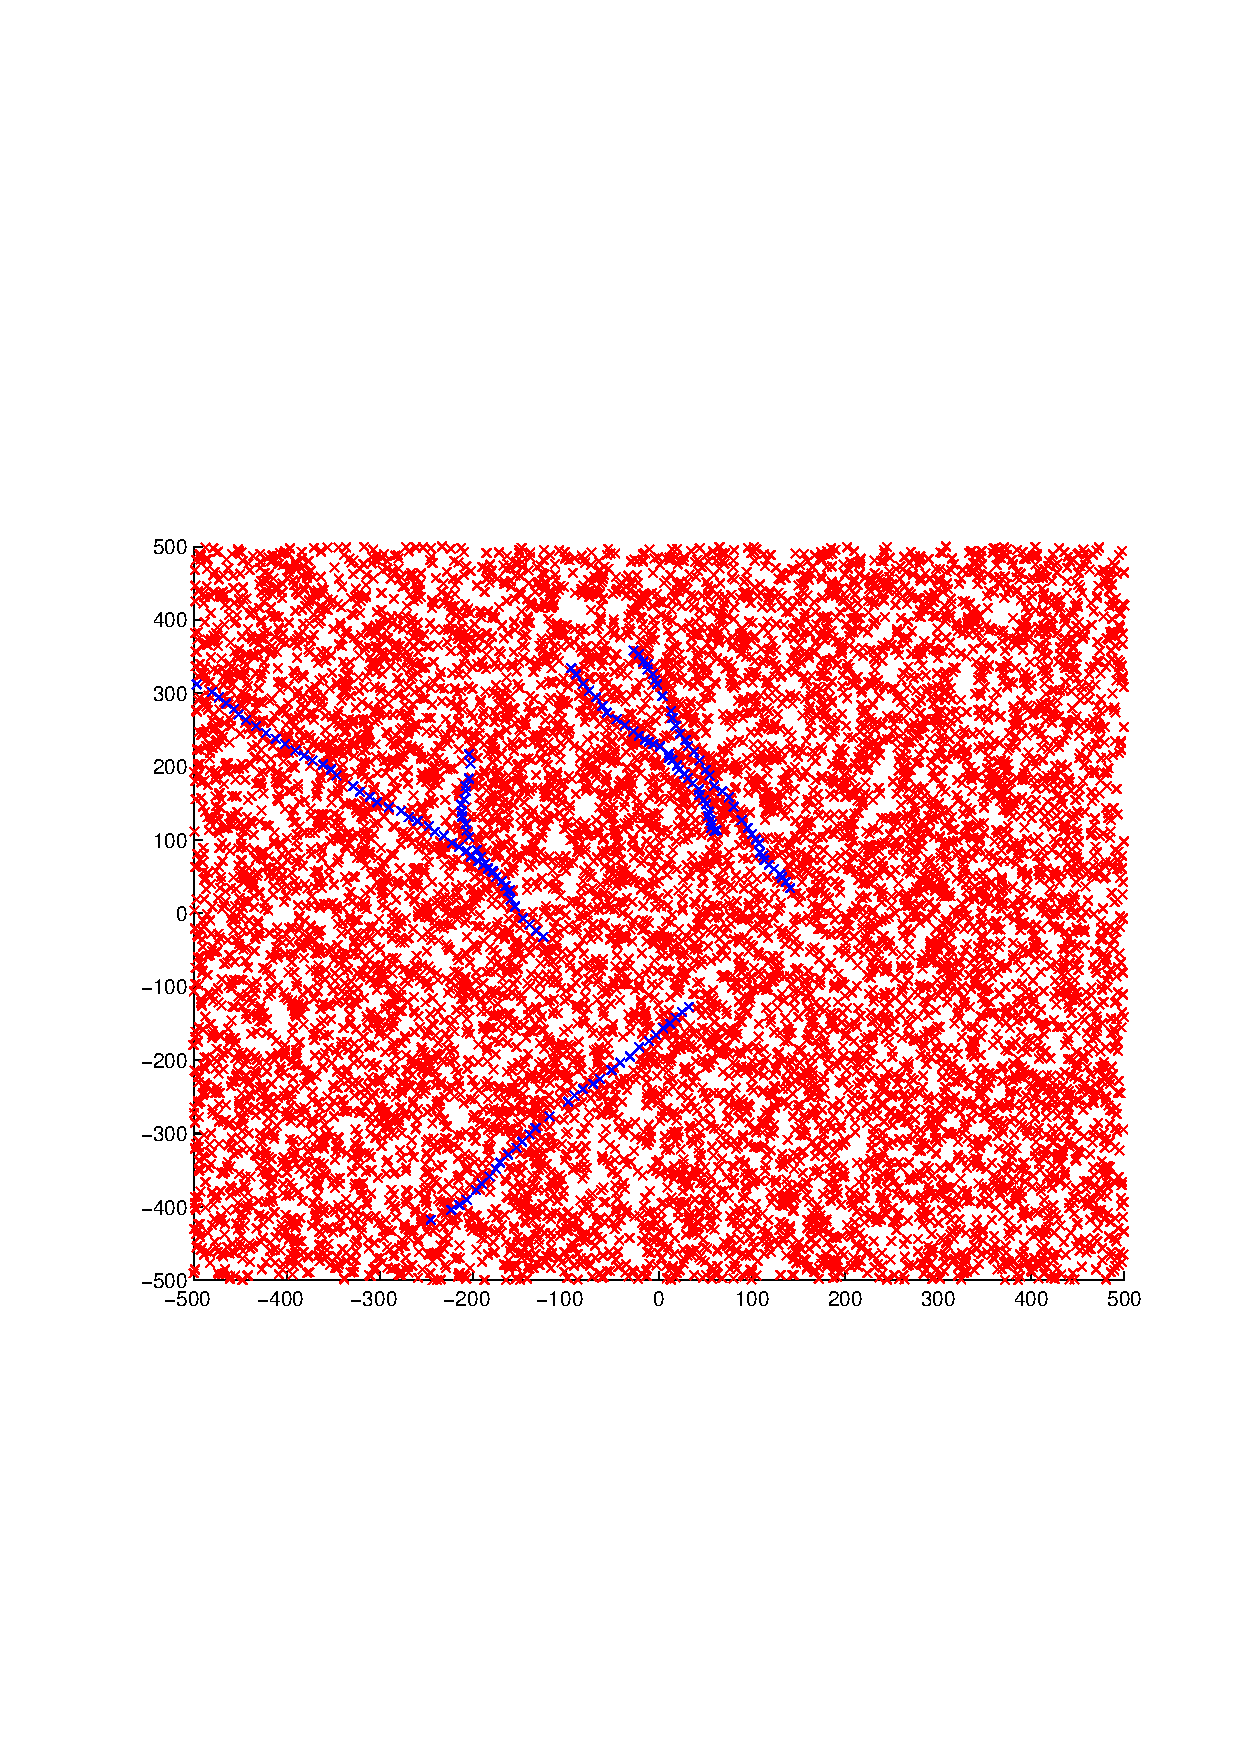
\includegraphics[width=0.45\columnwidth]{DetectionTrackingObs.pdf}}
\subfigure[States and Particle Estimates]{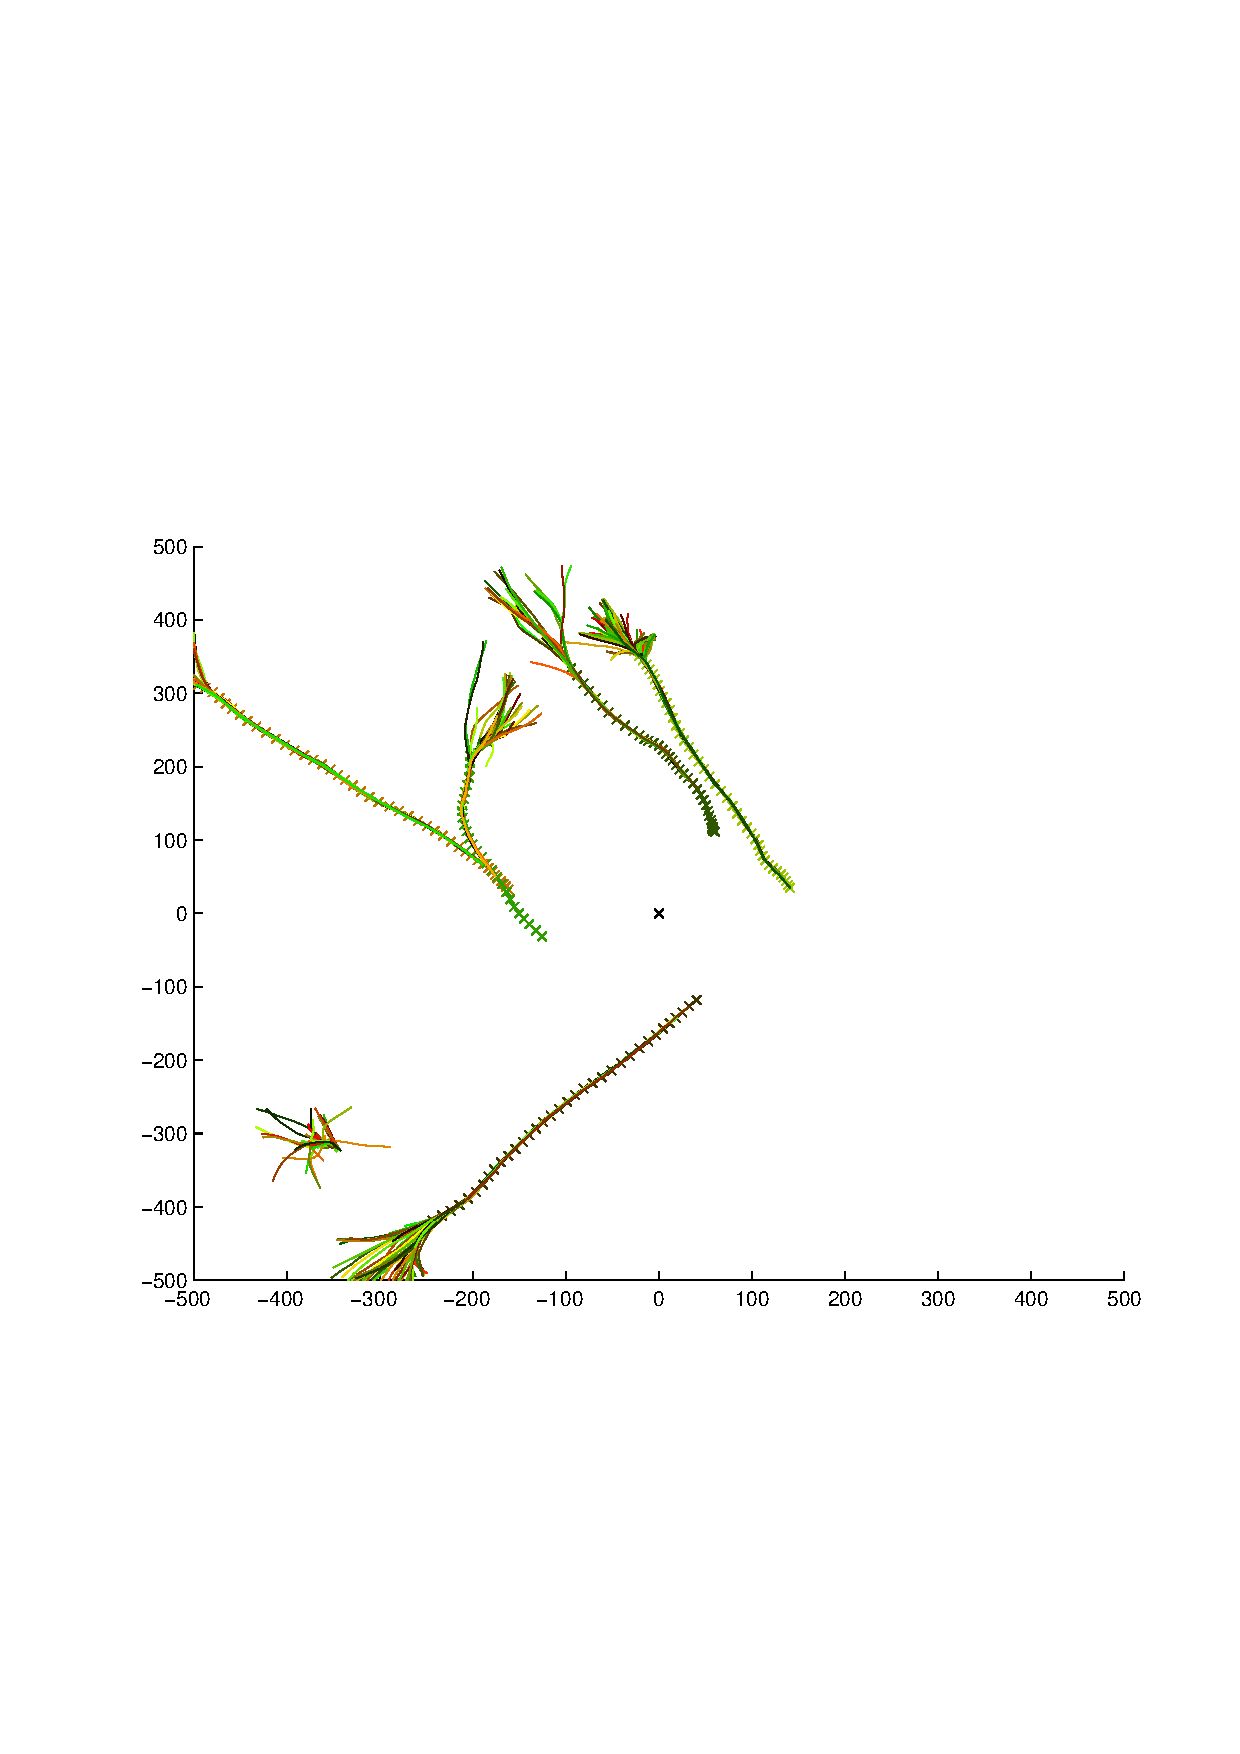
\includegraphics[width=0.45\columnwidth]{DetectionTracking.pdf}}
\caption{Target detection and tracking with fixed lag SISR algorithm with lag 5.}%
\label{fig:DetectionTracking}%
\end{figure}


\chapter{Results}
\section{Testing methods}
A number of algorithms were compared on a set of standard tests to compare the performance:

\begin{itemize}
	\item SISR
	\item SISR FL(5)
	\item RB-SISR FL(5)
	\item MCMC
	\item MCMC FL(5)
	\item RB-MCMC FL(5)
	\item PDAF
	\item JPDAF
\end{itemize}

where FL(N) indicates fixed lag with a window length of N and RB indicated Rao-Blackwellisation. The test set consisted of:

\begin{enumerate}
	\item 5 widely-spaced targets
	\item 5 widely-spaced targets, high clutter and missed detection rate
	\item 5 widely-spaced targets, high observation noise covariance
	\item 5 closely-spaced targets
\end{enumerate}

Each scenario lasted for 50 time steps. Each was tested using both the linear and bearing-range observation models. Each combination was run with 10 different random seeds. An example of each is shown in figures~\ref{fig:EgScen1} to~\ref{fig:EgScen4}.

\begin{figure}%
\subfigure[state]{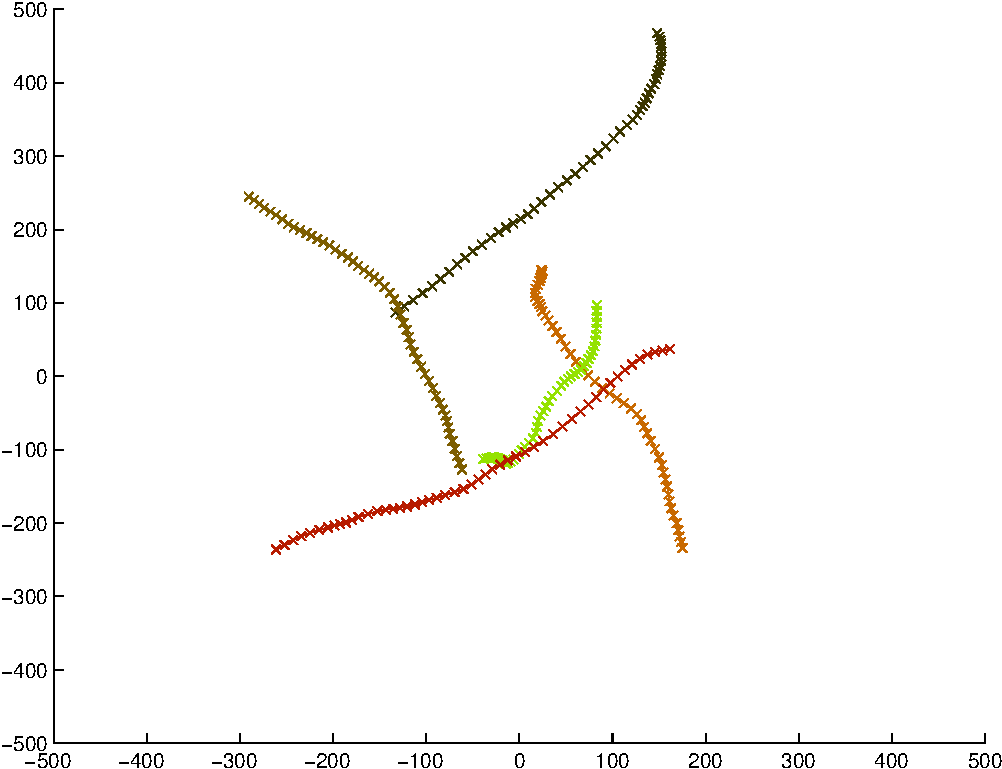
\includegraphics[width=0.3\columnwidth]{results_wide_low_state-crop.pdf}}
\subfigure[linear observations]{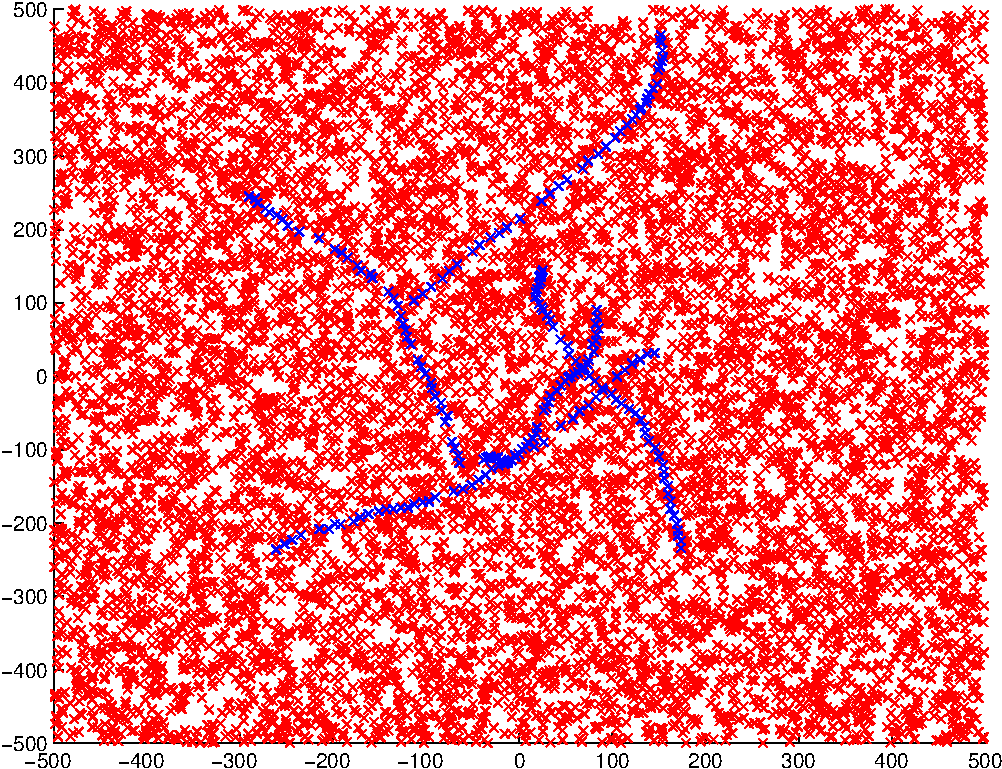
\includegraphics[width=0.3\columnwidth]{results_wide_low_lGobs-crop.pdf}}
\subfigure[bearing-range observations]{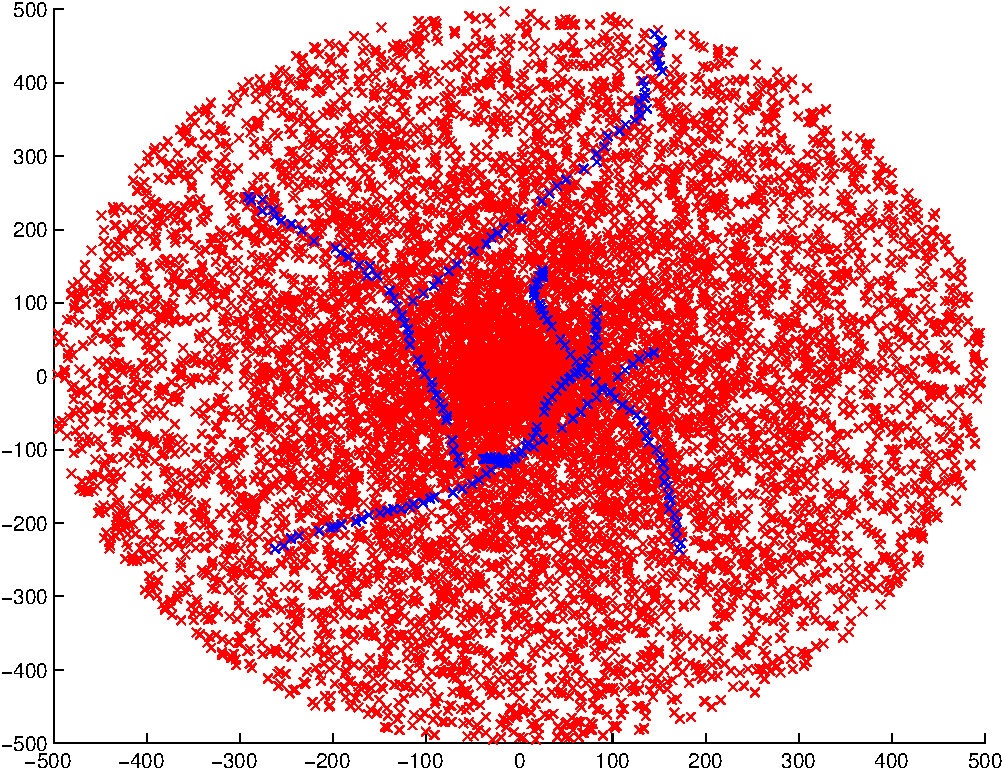
\includegraphics[width=0.3\columnwidth]{results_wide_low_brobs-crop.pdf}}
\caption{Case 1}%
\label{fig:EgScen1}%
\end{figure}
\begin{figure}%
\subfigure[state]{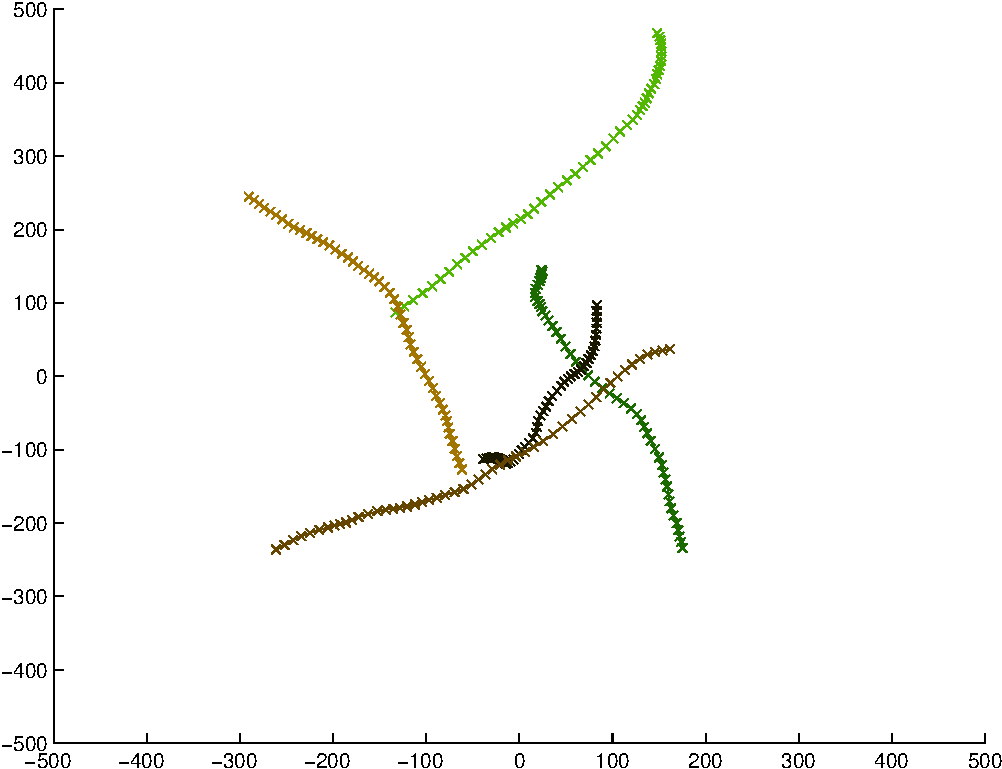
\includegraphics[width=0.3\columnwidth]{results_wide_high_state-crop.pdf}}
\subfigure[linear observations]{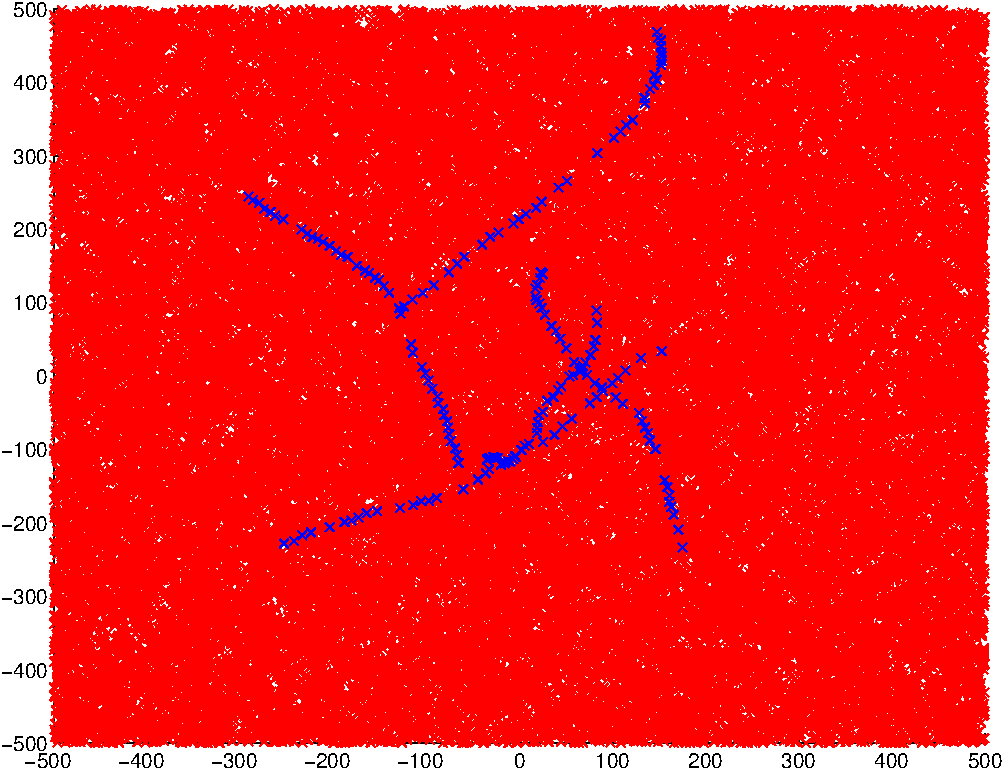
\includegraphics[width=0.3\columnwidth]{results_wide_high_lGobs-crop.pdf}}
\subfigure[bearing-range observations]{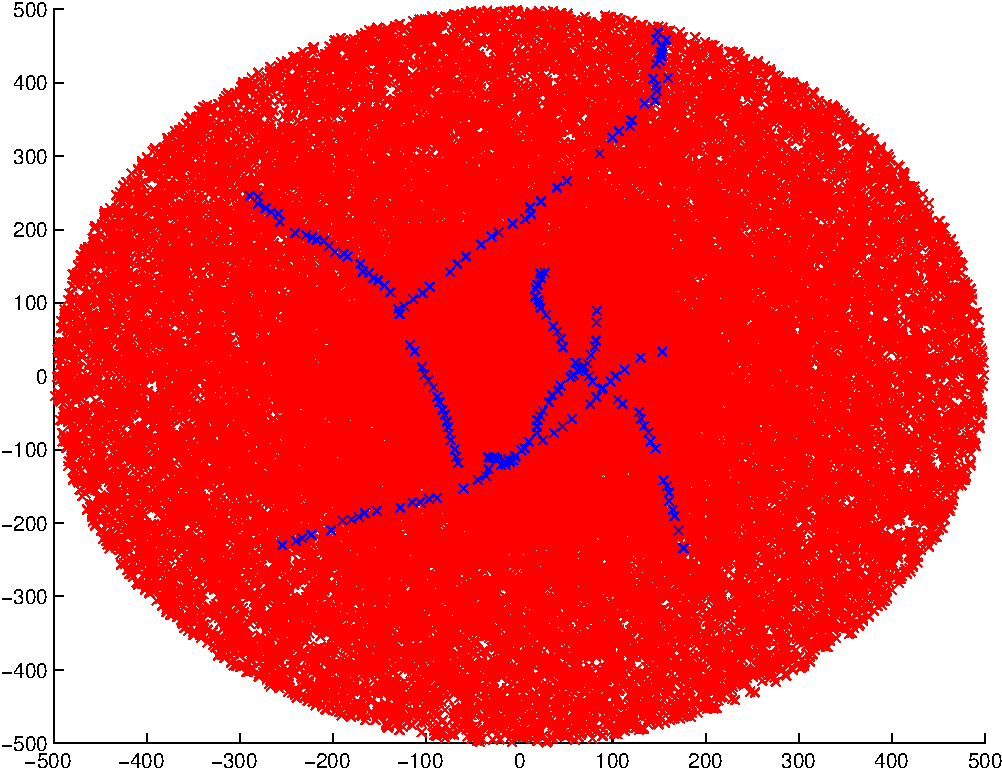
\includegraphics[width=0.3\columnwidth]{results_wide_high_brobs-crop.pdf}}
\caption{Case 2}%
\label{fig:EgScen2}%
\end{figure}
\begin{figure}%
\subfigure[state]{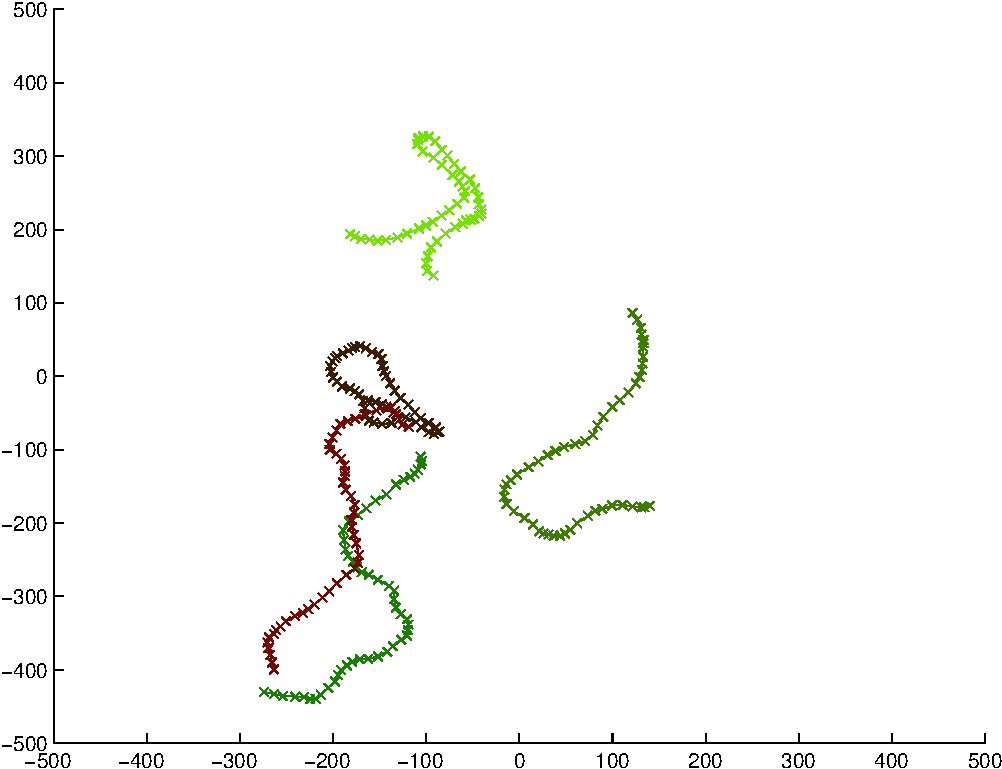
\includegraphics[width=0.3\columnwidth]{results_wide_noise_state-crop.pdf}}
\subfigure[linear observations]{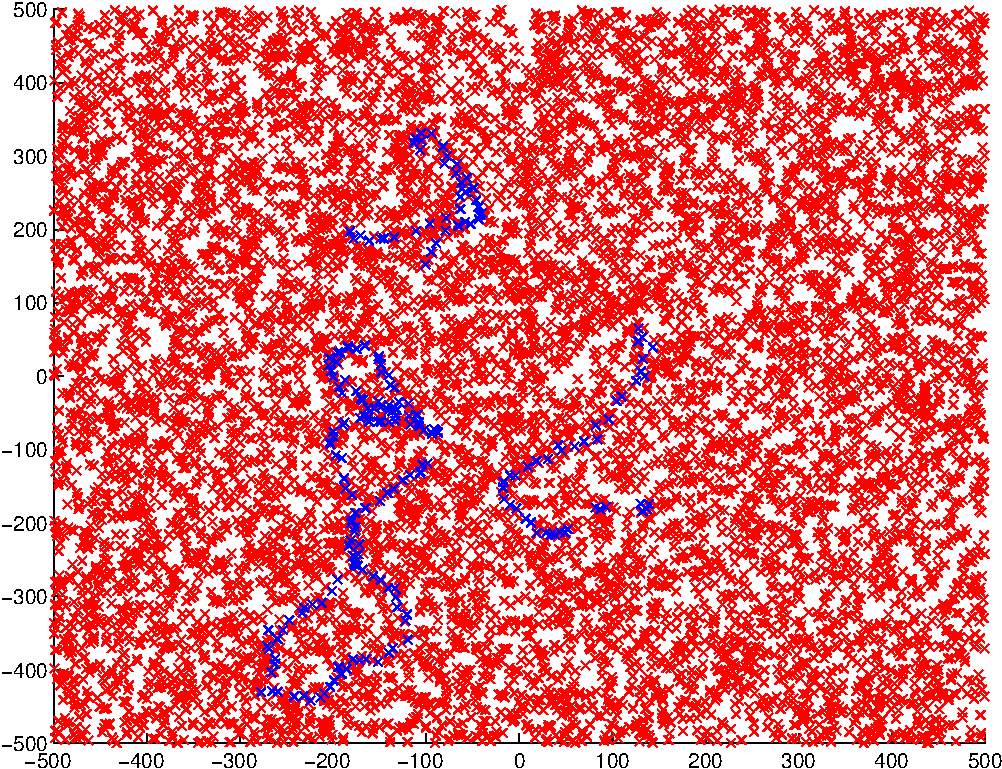
\includegraphics[width=0.3\columnwidth]{results_wide_noise_lGobs-crop.pdf}}
\subfigure[bearing-range observations]{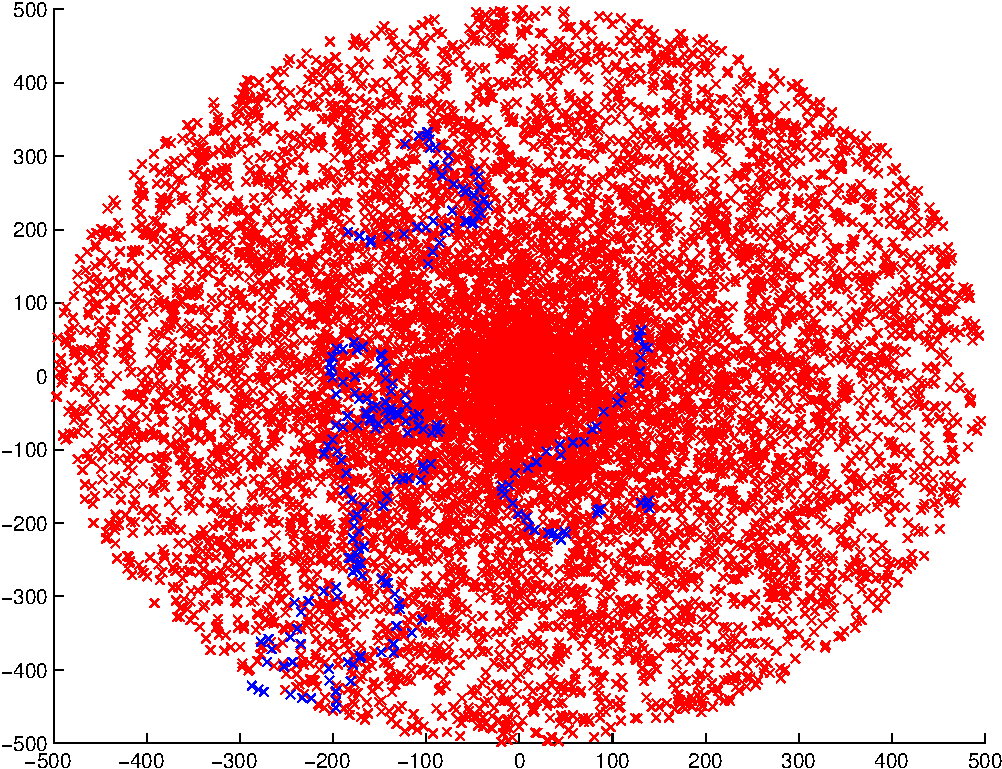
\includegraphics[width=0.3\columnwidth]{results_wide_noise_brobs-crop.pdf}}
\caption{Case 3}%
\label{fig:EgScen3}%
\end{figure}
\begin{figure}%
\subfigure[state]{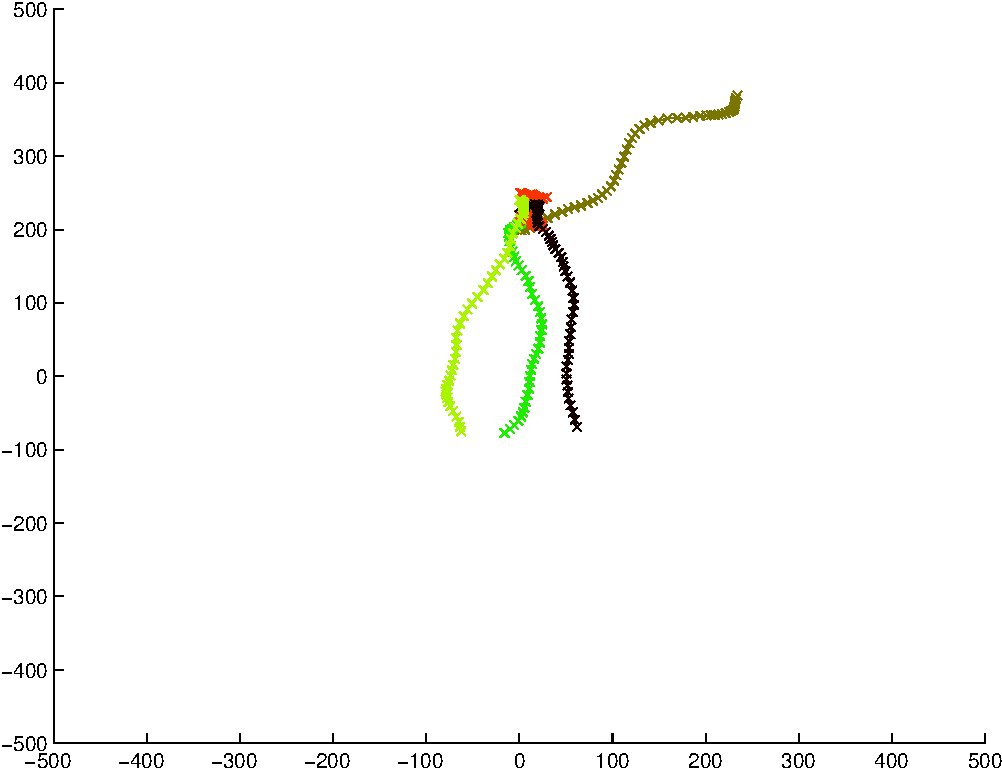
\includegraphics[width=0.3\columnwidth]{results_close_state-crop.pdf}}
\subfigure[linear observations]{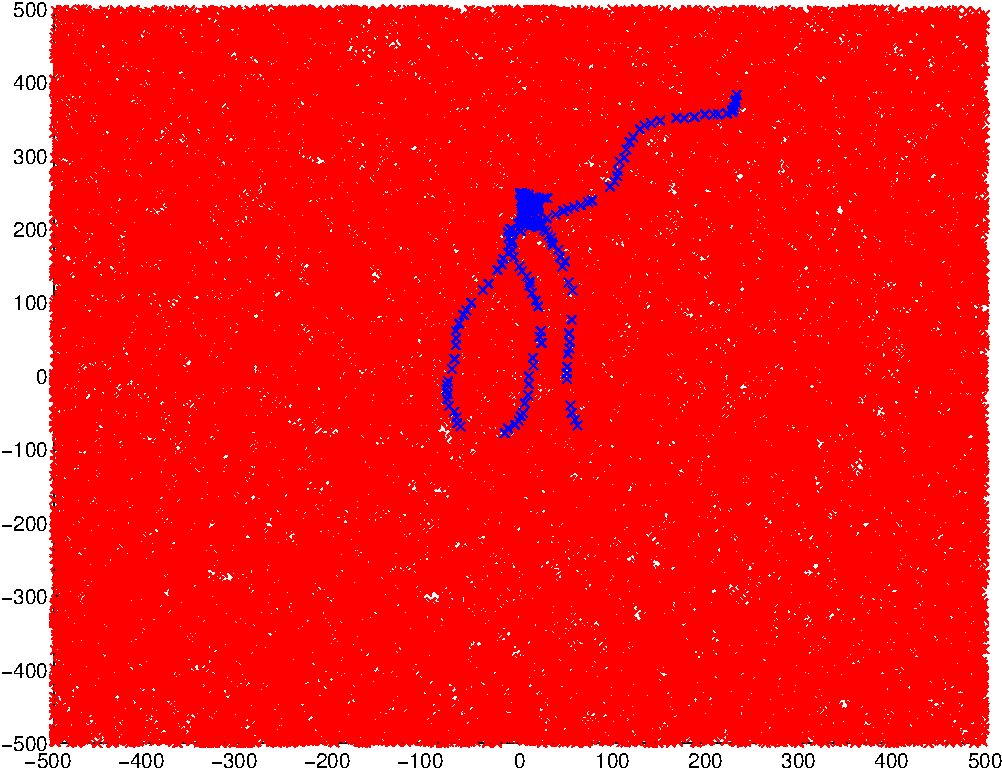
\includegraphics[width=0.3\columnwidth]{results_close_lGobs-crop.pdf}}
\subfigure[bearing-range observations]{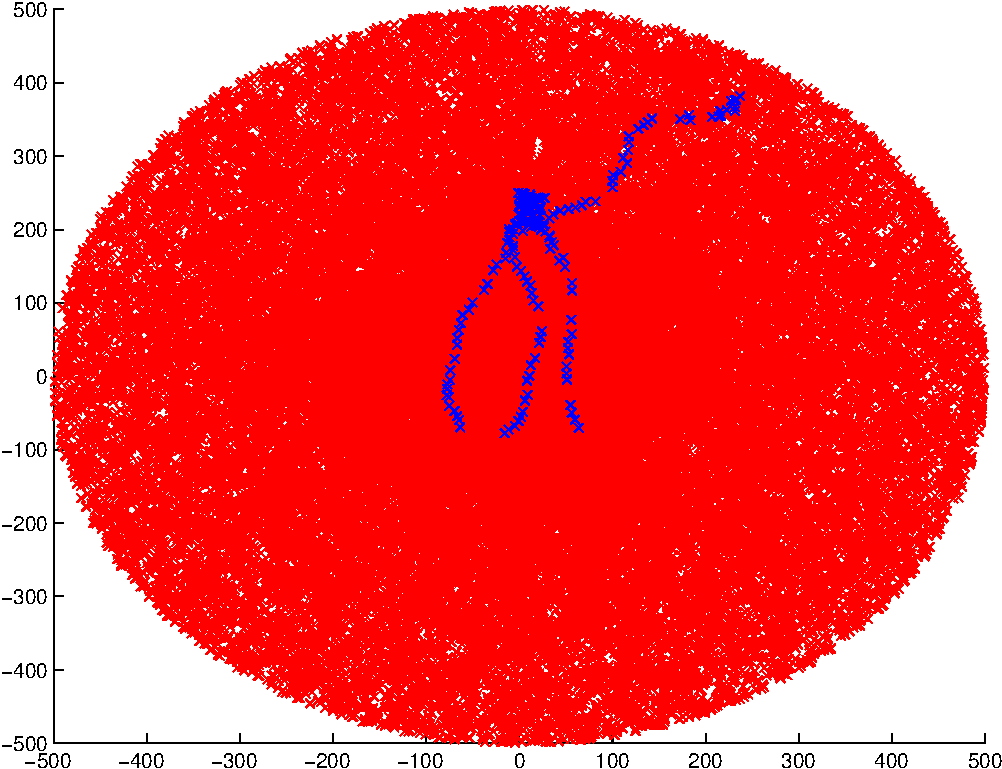
\includegraphics[width=0.3\columnwidth]{results_close_brobs-crop.pdf}}
\caption{Case 4}%
\label{fig:EgScen4}%
\end{figure}

Each scene is $1000 \times 1000$. The velocity of the targets is limited to 10. The period between time steps is 1. The case-specific parameters used are shown in table~\ref{tab:CaseParameters}

\begin{table}%
\begin{center}
\begin{tabular}{|c|c|c|c|c|}
\hline
 & case 1 & case 2 & case 3 & case 4 \\
\hline \hline
process variance & 1 & 1 & 10 & 1 \\
observation variance (linear) & 1 & 1 & 10 & 1 \\
bearing variance (nonlinear) & $10^{-4}$ & $10^{-4}$ & $10^{-3}$ & $10^{-4}$ \\
range variance (nonlinear) & 1 & 1 & 10 & 1 \\
expected no. clutter ($\mu_C$) & 200 & 1000 & 200 & 1000 \\
detection probability ($P_D$) & 0.9 & 0.75 & 0.9 & 0.75 \\
\hline
\end{tabular}
\end{center}
\caption{Table of parameters for each test case.}
\label{tab:CaseParameters}
\end{table}

The SISR algorithm was run with 500 particles per target. The MCMC algorithm used 5000 iterations and updated the targets in a deterministic order. All algorithms employed gating at 5 standard deviations using a normal approximation.
\section{Performance assessment}
Performance was assessed via a number of statistics. Firstly the number of lost tracks was counted. For the particle filter algorithms these were identified using the associations. When no particle was associated with the correct observation for five frames, the target was considered lost. For non-particle algorithms (PDAF and JPDAF), targets were considered lost when the mean state estimate was greater than a certain threshold distance from the correct position.

After excluding lost tracks, the root-mean-square state error (RMSE) was measured. For the particle algorithms a state estimate was obtained by taking the mean of the state of all particles. For non-particle algorithms, the mean of the Gaussian representing the state distribution was used. For particle algorithms, the proportion of particles with the correct association was also calculated. These statistics were all measured at a fixed lag of five steps from the current time, for consistency of comparison.

Results are shown in tables~\ref{tab:ResultsLinear} and~\ref{tab:ResultsRadar}. Blank cells indicate that the tracker failed to complete the test in a reasonable time. With the JPDAF this occurred when the number of association hypotheses grew too large.

\begin{table}[!p] \centering
\begin{tabular}{|c|c|c|c|c|c|}
\hline
 & & \multicolumn{4}{|c|}{Algorithm} \\
\hline
 & & Case 2 & Case 1 & Case 3 & Case 4 \\
\hline
\multirow{3}{*}{PDAF} & lost tracks             & 32\% & 4\% & 56\% & 50\% \\
                         & RMSE                 & 4.00 & 1.57 & 5.93 & 4.12 \\
\hline
\multirow{3}{*}{JPDAF} & lost tracks            &  & 4\% & 48\% &  \\
                         & RMSE                 &  & 1.57 & 5.89 &  \\
\hline
\multirow{3}{*}{SISR(1)} & lost tracks          & 32\% & 2\% & 100\% & 36\% \\
                         & RMSE                 & 5.53 & 1.39 &  & 7.46 \\
                         & correct associations & 72\% & 93\% &  & 63\% \\
\hline
\multirow{3}{*}{SISR(5)} & lost tracks          & 2\% & 0\% & 42\% & 16\% \\
                         & RMSE                 & 2.02 & 0.95 & 50.12 & 2.01 \\
                         & correct associations & 85\% & 93\% & 71\% & 79\% \\
\hline
\multirow{3}{*}{RB-SISR(5)} & lost tracks       & 4\% & 0\% & 12\% & 12\% \\
                         & RMSE                 & 1.95 & 1.36 & 9.01 & 2.90 \\
                         & correct associations & 86\% & 93\% & 86\% & 83\% \\
\hline
\multirow{3}{*}{MCMC(1)} & lost tracks          & 30\% & 2\% & 100\% & 38\% \\
                         & RMSE                 & 2.24 & 1.04 &  & 1.74 \\
                         & correct associations & 87\% & 99\% &  & 81\% \\
\hline
\multirow{3}{*}{MCMC(5)} & lost tracks          & 26\% & 0\% & 100\% & 26\% \\
                         & RMSE                 & 1.44 & 0.98 &  & 1.47 \\
                         & correct associations & 87\% & 99\% &  & 81\% \\
\hline
\multirow{3}{*}{RB-MCMC(5)} & lost tracks       & 6\% & 0\% & 10\% & 12\% \\
                         & RMSE                 & 2.31 & 1.33 & 3.35 & 1.81 \\
                         & correct associations & 91\% & 99\% & 90\% & 90\% \\
\hline
\end{tabular}
\caption{Algorithm test performance measures for linear observation model}
\label{tab:ResultsLinear}
\end{table}

\begin{table}[!p] \centering
\begin{tabular}{|c|c|c|c|c|c|}
\hline
 & & \multicolumn{4}{|c|}{Algorithm} \\
\hline
 & & Case 2 & Case 1 & Case 3 & Case 4 \\
\hline
\multirow{3}{*}{PDAF} & lost tracks             & 60\% & 8\% & 80\% & 72\% \\
                         & RMSE                 & 4.89 & 2.96 & 10.15 & 5.98 \\
\hline
\multirow{3}{*}{JPDAF} & lost tracks            &  & 6\% &  &  \\
                         & RMSE                 &  & 2.95 &  &  \\
\hline
\multirow{3}{*}{SISR(1)} & lost tracks          & 40\% & 10\% & 100\% & 50\% \\
                         & RMSE                 & 9.86 & 2.54 &  & 12.93 \\
                         & correct associations & 57\% & 86\% &  & 50\% \\
\hline
\multirow{3}{*}{SISR(5)} & lost tracks          & 16\% & 4\% & 82\% & 22\% \\
                         & RMSE                 & 4.51 & 1.54 & 67.9 & 5.91 \\
                         & correct associations & 71\% & 90\% & 55\% & 69\% \\
\hline
\multirow{3}{*}{RB-SISR(5)} & lost tracks       & 18\% & 6\% & 30\% & 26\% \\
                         & RMSE                 & 4.21 & 1.86 & 16.91 & 4.99 \\
                         & correct associations & 71\% & 89\% & 68\% & 72\% \\
\hline
\multirow{3}{*}{MCMC(1)} & lost tracks          & 30\% & 2\% & 100\% & 52\% \\
                         & RMSE                 & 4.32 & 1.73 &  & 3.54 \\
                         & correct associations & 75\% & 98\% &  & 68\% \\
\hline
\multirow{3}{*}{MCMC(5)} & lost tracks          & 20\% & 4\% & 100\% & 44\% \\
                         & RMSE                 & 3.21 & 1.52 &  & 3.11 \\
                         & correct associations & 79\% & 97\% &  & 71\% \\
\hline
\multirow{3}{*}{RB-MCMC(5)} & lost tracks       & 22\% & 2\% & 48\% & 36\% \\
                         & RMSE                 & 3.36 & 1.78 & 5.96 & 3.18 \\
                         & correct associations & 80\% & 96\% & 65\% & 74\% \\
\hline
\end{tabular}
\caption{Algorithm test performance measures for bearing-range observation model}
\label{tab:ResultsRadar}
\end{table}

Figures~\ref{fig:Tracking_PDAF} to~\ref{fig:Tracking_MCMC} show the comparative performance of the algorithms on a few example cases.

\begin{figure} \centering
\subfigure[PDAF]{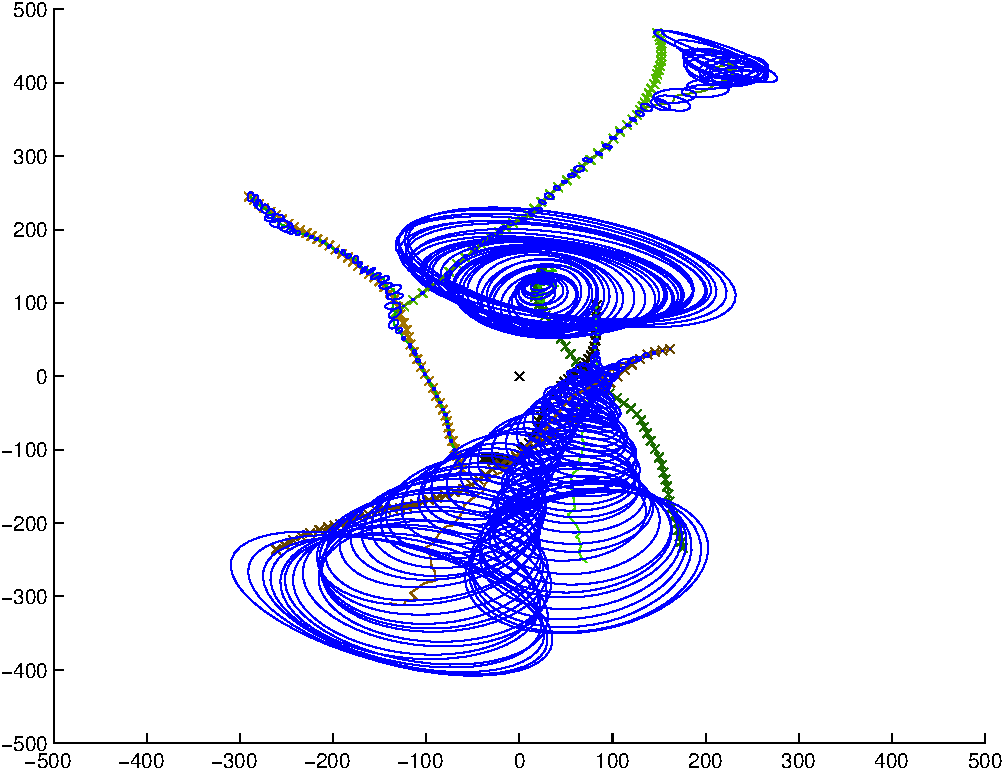
\includegraphics[width=0.49\columnwidth]{results_PDAF-crop.pdf}}
\caption{PDAF tracking results. Ellipses mark 1 standard deviation from the mean from the Gaussian covariance estimate.}%
\label{fig:Tracking_PDAF}%
\end{figure}

\begin{figure} \centering
\subfigure[SISR(1)]{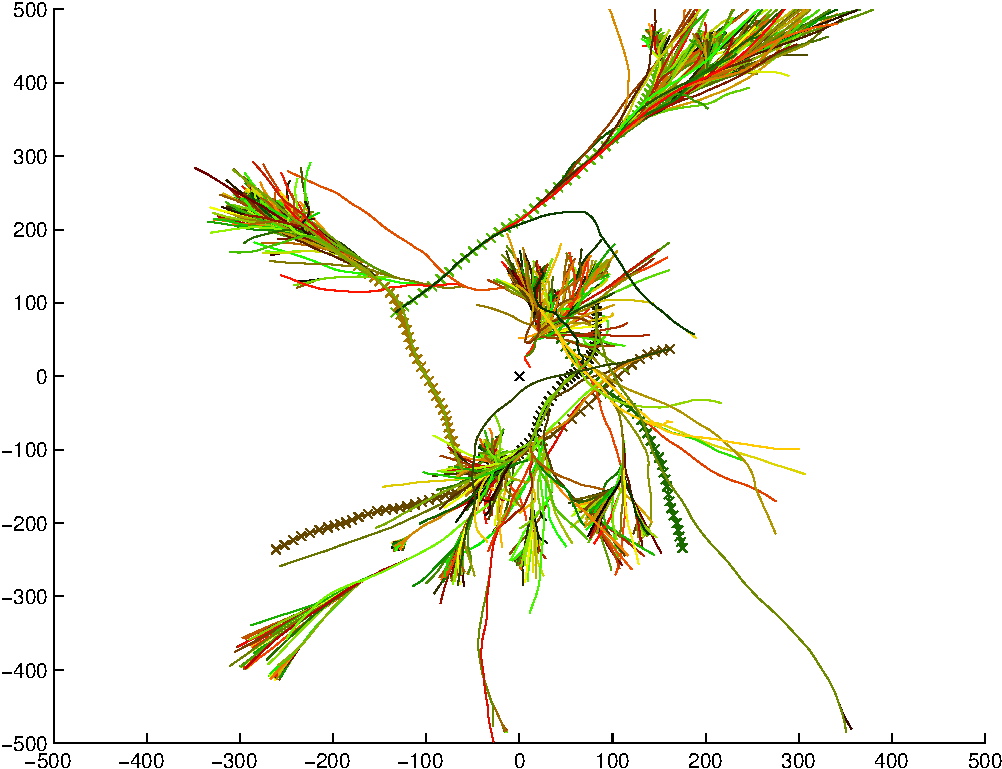
\includegraphics[width=0.49\columnwidth]{results_SISR1-crop.pdf}}
\subfigure[SISR(5)]{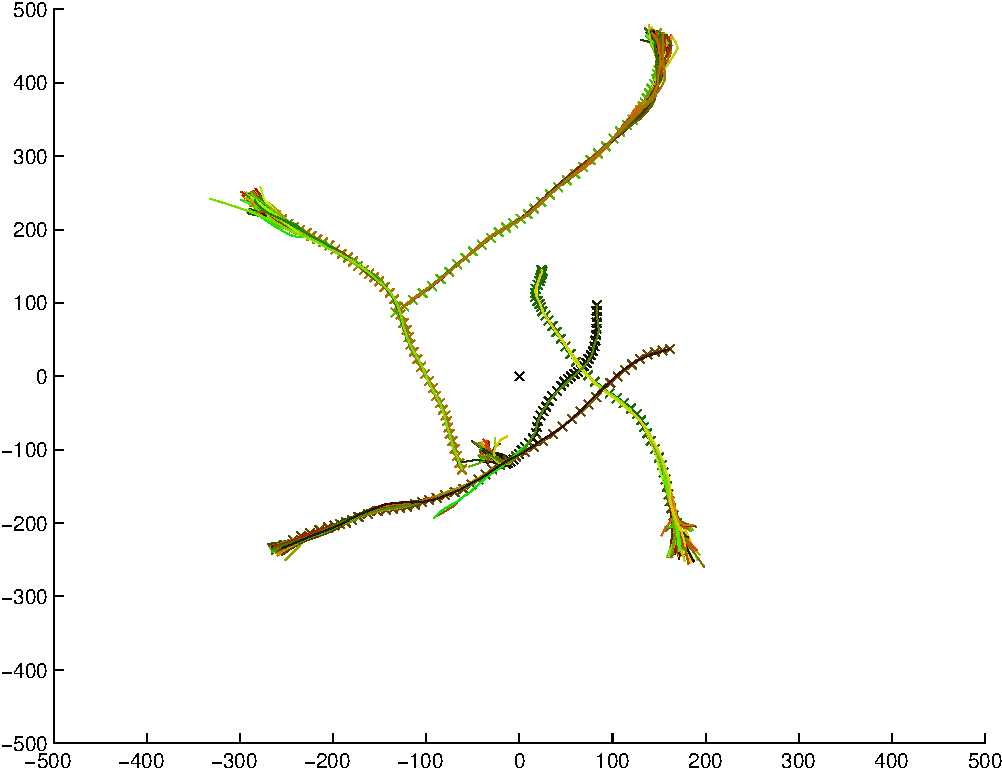
\includegraphics[width=0.49\columnwidth]{results_SISR5-crop.pdf}} \\
\subfigure[RB-SISR(5)]{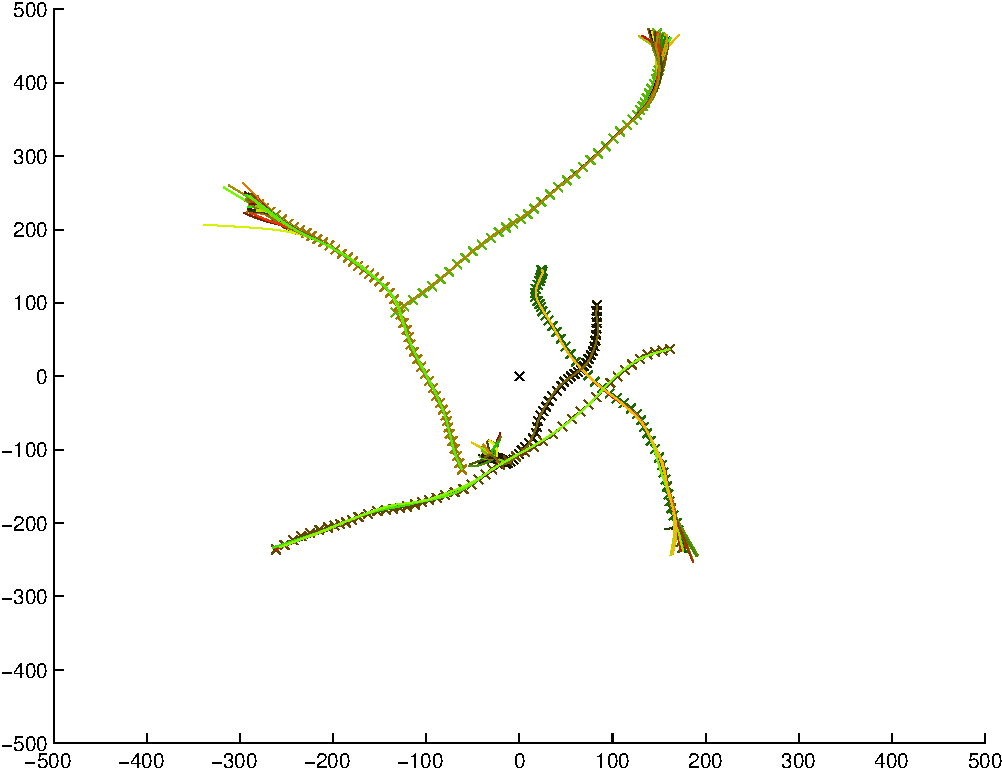
\includegraphics[width=0.49\columnwidth]{results_RB-SISR5-crop.pdf}}
\caption{SISR tracking results. All particles plotted.}%
\label{fig:Tracking_SISR}%
\end{figure}

\begin{figure} \centering
\subfigure[MCMC(1)]{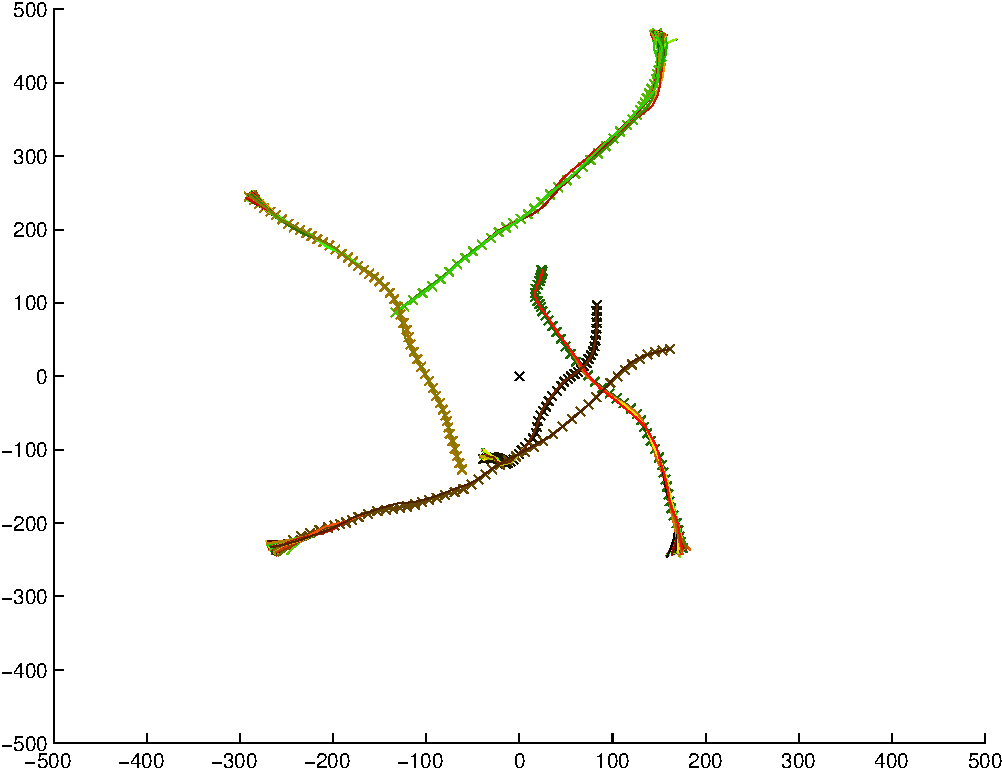
\includegraphics[width=0.49\columnwidth]{results_MCMC1-crop.pdf}}
\subfigure[MCMC(5)]{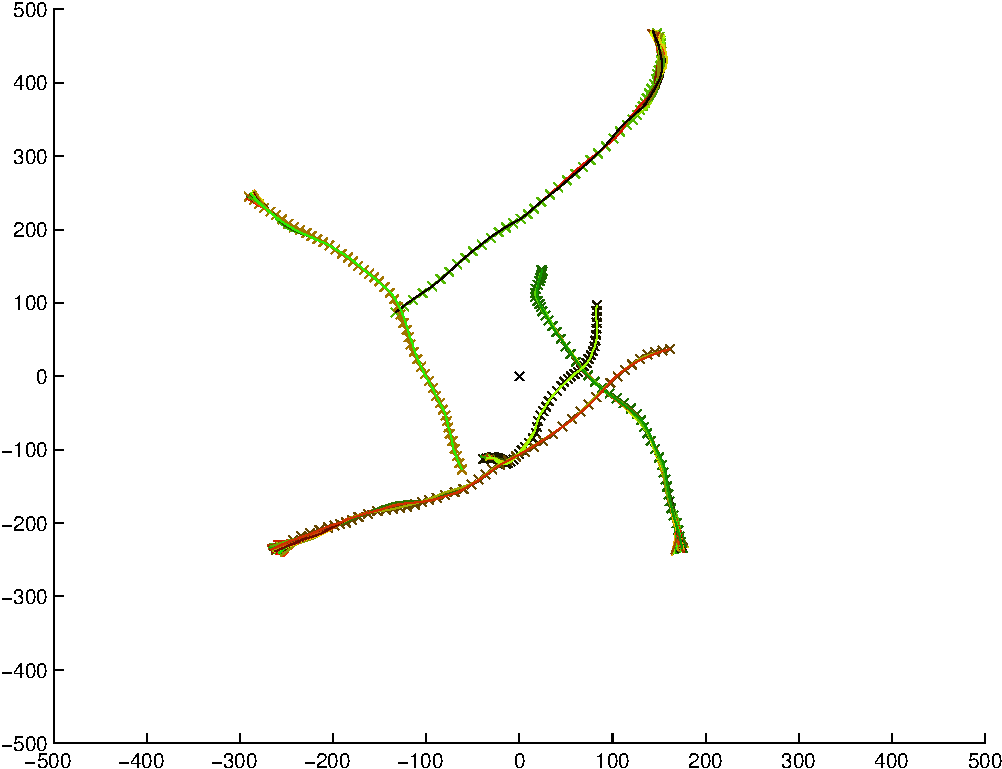
\includegraphics[width=0.49\columnwidth]{results_MCMC5-crop.pdf}} \\
\subfigure[RB-MCMC(5)]{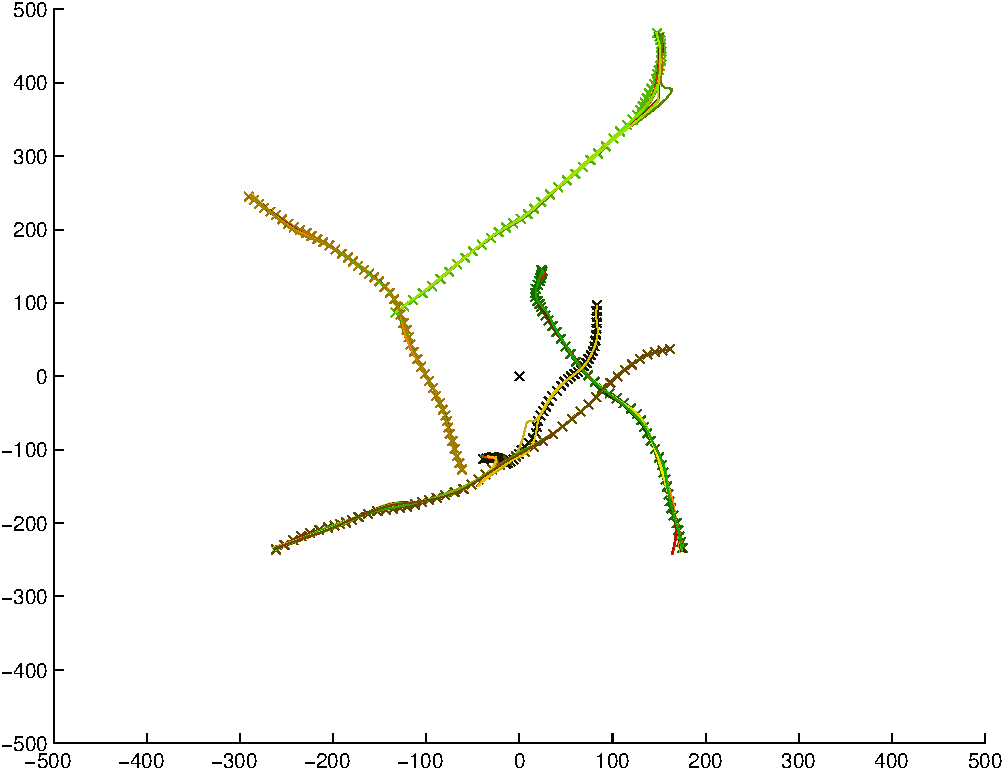
\includegraphics[width=0.49\columnwidth]{results_RB-MCMC5-crop.pdf}}
\caption{MCMC tracking results. All particles plotted.}%
\label{fig:Tracking_MCMC}%
\end{figure}

These results highlight the characteristics of the fixed lag particle filters. In almost all cases the particle algorithms outperform the basic PDAF tracker in terms of number of tracks lost and RMSE. In all cases using a longer window results in better tracking performance. Tracking performance is always better with the linear observation model rather than the bearing-range model. For the linear model, no Gaussian approximations are needed and the proposal distributions are optimal.

For the linear observation model, the use of Rao-Blackwellisation seems to give a reduction in the number of tracks lost, and makes little difference to the RMSE. This is the expected result. The Kalman filters used for state estimation are optimal for this model, and the reduction in dimensionality means that low probability paths are better characterised, resulting in fewer track losses. With the bearing-range observation model, the reduction in lost tracks from Rao-Blackwellisation is less. This could be because the Kalman filter estimates are no longer optimal, resulting in worse state estimates and a greater tendency to follow an incorrect path. However, this hypothesis is not born out in the RMSE results, which are not significantly worse than the full particle filter.

For case 3, with high process and observation noise, the full particle filters do not work at all, while the Rao-Blackwellised forms give good tracking performance. This is because of the number of particles used is insufficient to characterise the state distribution well. The probability of getting a `good' particle becomes low, so tracks are lost very quickly. The marginalised particle filter does not need to characterise the state distribution, so the increased variance is not so significant.

On the widely spaced targets, the SISR-PFs suffer from fewer lost tracks than the MCMC-PFs. This appears to be caused by two related effects. The SISR particles are generated independently, and with the conservative resampling scheme employed a number of particles will be maintained with low weights on low probability paths. If these paths turn out to be correct, the tracker will not lose the target. The MCMC particles fail to maintain a particle contribution on such low probability paths. This may be because the particles are generated sequentially, each based upon the previous. Moves to low probability paths simply never get accepted. This problem can be viewed in an alternative light. After a few additional time steps, a low probability path which is actually correct will increase again in probability. We would like the MCMC sampler to then be able to jump across to this path. However, to do so will generally require a move in which all the states in the window (from the point at which the potential path bifurcated until the present) change significantly. Such a high dimensional move will have a very low acceptance probability, and the chains used may simply not be long enough.

Disappointingly, the MCMC-PFs do not seem to give an improvement in track loss over the SISR-PFs for the closely-spaced targets. Seeing as the MCMC-based tracker maintains a full joint distribution, it might be expected to suffer from fewer merged or crossing-over tracks. However, the difficulties outlined above seem to outweigh this potential advantage.

The particle based algorithms are of the order of 1000 times slower than the PDAF, i.e. the same order as the number of particles used. The computation time scales linearly with the length of the window. The scaling with the number of targets depends on how they interact with each other. Targets which are essentially independent (i.e. well-spaced), give rise to a linear scaling. For closely-spaced targets, the number of particles will have to increase more than linearly with the number of targets to maintain a constant level of tracking performance. The use of Rao-Blackwellisation gives the potential for a significant speed-up because many more calculations will be repeated between particles. However, this potential was not exploited in this work. The JPDAF is, while all targets remain in track, almost as fast as the PDAF. However, with a naive implementation, such as that used for these tests, the computation time explodes when a track is lost (due to the widening variance of the estimated state resulting in an increasing number of observations lying in each gate). More intelligent approaches can avoid such problems, e.g. \cite{Horridge2006}.

\chapter{Plan Of Future Research}
A number of possible extensions to the current work are envisaged. Firstly, there are a number of variants of the particle filtering algorithms which would be interesting to investigate. Secondly, there are numerous additional problems in tracking which could be addressed. Finally, the fixed lag particle filter approach could be applied to different applications entirely.



\section{Ideas for improved particle filters}

\subsection{Mixed exact-flow filter}
In a traditional particle filter, particles are propagated from one time step to the next through the use of a proposal distribution and a weighting step, with resampling to maintain diversity. In \cite{Daum2010}, the authors introduce a new sort of particle filter, in which particles are propagated as if they were diffusing according a differential equation governed by the observation likelihood. Thus, it is possible to generate an exact, unweighted sample from the desired posterior distribution even for a nonlinear, non-Gaussian model. This method cannot be directly applied to a target tracking problem because such particle flow ideas can only be used for continuous state-spaces. The association variables will need to be handled differently.

It seems intuitive that we may be able to use an exact-flow filter for the kinematic target states, $X_t$, and an ordinary particle filter for the associations, $\Lambda_t$, in a similar manner to the Rao-Blackwellised method where a Kalman filter or filters is used for the kinematic states.

Consider a single target with state $x_t$ and associations $\lambda_t$. From the previous processing step we have a particle approximation for the posterior, $\hat{P}(x_{1:t-1}, \lambda_{1:t-1}|Y_{1:t-1})$. The exact-flow method allows us to generate a sample from $P(x_t|x_{t-1}, \lambda_t, Y_t)$. Thus, a new particle set can be generated from the following proposal

\begin{equation}
x_{1:t}^{(m)},\lambda_{1:t}^{(m)} \sim \hat{P}(x_{1:t-1}, \lambda_{1:t-1}|Y_{1:t-1}) q(\lambda_t|X_{t-1}, Y_t) P(x_t|x_{t-1}, \lambda_t, Y_t)
\end{equation}

The same association proposal may be used as for the standard particle filters described in chapter~\ref{}. Note that this proposal implicity includes a resampling step, which could be omited, as always. The importance weights for such a filter will be given by

\begin{IEEEeqnarray}{rCl}
W_t^{(m)} & \approx & \frac{ P(x_{1:t}^{(m)}, \lambda_{1:t}^{(m)}|Y_{1:t}) }{ P(x_{1:t-1}, \lambda_{1:t-1}|Y_{1:t-1}) q(\lambda_t|X_{t-1}, Y_t) P(x_t|Y_{1:t}, \lambda_t) } \\
 & = & \frac{ P(\lambda_t^{(m)}) P(Y_t|x_{t-1}^{(m)},\lambda_t^{(m)}) }{ P(Y_t|Y_{1:t-1}) q(\lambda_t|X_{t-1}, Y_t) }
\end{IEEEeqnarray}

Unfortuneately, the $P(Y_t|x_{t-1}^{(m)},\lambda_t^{(m)})$ term will not be tractable in general. However, a Monte Carlo approximation could be used.

\begin{equation}
P(Y_t|x_{t-1},\lambda_t) = \int P(Y_t|x_{t},\lambda_t) P(x_t|x_{t-1}) dx_t \approx \sum_i P(Y_t|x_t^{(i)}, \lambda_t)
\end{equation}

where the summation is over a set of particles sampled from $P(x_t|x_{t-1})$. This of course leads to an algorithm with $O(N^2)$ complexity in the number of particles as a Monte Carlo approximation is needed for each particle in the main filter. However, provided both the transition density and the likelihood have a simple, unimodal form, the inner approximation may require only a small number of particles, rendering the scheme tractable.



\subsection{SISR proposals for MCMC}
The main failure mode of the MCMC-PF tracker occurs when there are two possible convincing routes for a target to take - generally one correct but with some missed detections and one marked by an unfortunate chain of clutter observations. The sampler gets onto the wrong path (is often initialised in it) and fails to jump to the other.

The SISR-PF tracker does not have this problem, because the particles are generated in parallel. However, it only achieves acceptable performance if independence assumptions are introduced to reduce the dimensionality - effectively to run an independent PF on each target.

It may be possible to combine the two schemes. First, taking the particle distribution from the previous processing step, a set of independent SISR-PFs can be run. The resulting marginal distributions may then be used as proposal distributions for moves in a joint-target MCMC-PF. Such a scheme may benefit from the advantages of the two different algorithms, maintaining a complete joint representation of the target space while minimising track loss. Furthermore, if the right set of values from the independent filters are stored in memory there is very little additional calculation required for the joint-target MCMC-PF stage.

Such an algorithm is likely to fail when many targets are close together. In such a case, many of the proposals will result in association contradictions, and the MH acceptance rate will fall. Such invalid proposals can be rejected very quickly as we only need to check target associations rather than calculate transition or likelihood probabilities. Thus, we can mitigate this problem by simply lengthening the chain.



\subsection{MCMC importance sampling}
The weakness of the MCMC-PF can be viewed in an another way. When the probability of the correct path is low, the SISR-PF is able to maintain it in the particle distribution with a number of low-weight particles until its probability rises again. In an MCMC scheme, all particles have equal weights, and such low-probability modes may get very few or no particles. An alternative way to combine the advantages of the SISR and MCMC methods would be to construct a Markov chain which generated a weighted particle distribution.

In an SISR scheme, a set of weighted particles $\{ x_{1:t}^{(m)}, W_t^{(m)} \}$ are used to approximate the posterior distibution, $P(x_{1:t}|Y_{1:t})$. The unweighted particles may be considered to be samples from some underlying distribution, $\mu(x_{1:t}|Y_{1:t})$ (determined by the proposal distribution and previous resampling steps). Potentially, a Markov chain could be targetted on $\mu(x_{1:t}|Y_{1:t})$ instead of $P(x_{1:t}|Y_{1:t})$.

Suppose at the $m^{\text{th}}$ step in the chain we have the state $x_{1:t}^{(m)}$, with unnormalised weight $W_t^{(m)}$. A new state, $x_{1:t}^{*}$ is sampled from a MH proposal distribution $q(.|x_{1:t}^{(m)}, Y_{1:t})$. The standard acceptance probability formula will be

\begin{equation}
\alpha = \min \bigg \{ 1, \frac{\mu(x_{1:t}^{*}|Y_{1:t})q(x_{1:t}^{(m)}|x_{1:t}^{*}, Y_{1:t})}{\mu(x_{1:t}^{(m)}|Y_{1:t})q(x_{1:t}^{*}|x_{1:t}^{(m)}, Y_{1:t})} \bigg \}
\end{equation}

For any given particle, we know that $P(x_{1:t}^{(m)}|Y_{1:t}) = W_t^{(m)} \mu(x_{1:t}^{(m)}|Y_{1:t})$ by definition, so

\begin{equation}
\alpha = \min \bigg \{ 1, \frac{W_t^{(m)}}{W_t^{*}} \times \frac{P(x_{1:t}^{*}|Y_{1:t})q(x_{1:t}^{(m)}|x_{1:t}^{*}, Y_{1:t})}{P(x_{1:t}^{(m)}|Y_{1:t})q(x_{1:t}^{*}|x_{1:t}^{(m)}, Y_{1:t})} \bigg \}
\end{equation}

But with this formulation $W_t^{*}$ is unknown. In fact, it could be set to anything: $\mu(x_{1:t}|Y_{1:t})$ is defined by $P(x_{1:t}|Y_{1:t})$ and the choice of weights rather than vice versa. An obvious choice of weight is to select

\begin{equation}
W_t^{*} = W_t^{(m)} \times \frac{P(x_{1:t}^{*}|Y_{1:t})q(x_{1:t}^{(m)}|x_{1:t}^{*}, Y_{1:t})}{P(x_{1:t}^{(m)}|Y_{1:t})q(x_{1:t}^{*}|x_{1:t}^{(m)}, Y_{1:t})}
\end{equation}

which results in an acceptance probability of 1 for all moves.

One possible choice of proposal would be to select a state history, $x_{1:t-1}$ from the previous particle distribution, $\hat{P}(x_{1:t-1}|Y_{1:t-1})$, and a current state dependent on this. This would result in a recursive cancellation in the particle weights, leading to (assuming $W_t^{(0)}=0$):

\begin{equation}
W_t^{*} = \frac{P(Y_t|x_t^{*})P(x_t^{*}|x_{t-1}^{*})}{q(x_{t}^{*}|x_{1:t-1}^{*}, Y_{t})}
\end{equation}

which is just the normal weight update formula for a simple SISR particle filter! However, we need not necessarily propose an entire new state for every particle, but can change one component (target) at a time. The result will be an SISR-like algorithm in which particles and weights are not generated independently but dependent on the previous particle and weight. In addition, we can choose different forms for the weight update equation. At the other end of the spectrum, we could set $W_t^{*}=1$ which gives us a standard MCMC-PF. Other choices could give some sort of intermediate filter which would allow some variation in weight but not as much as the SISR version.

The hope is that such a scheme should allow us to maintain a complete joint-target posterior distribution and yet not lose track of targets whose path is temporarily of low probability. However, it may simply suffer from all the problems of a joint-target SISR-PF. Specifically, it may discard particles with good estimates of one target because their estimates of another target are poor. In any case, it seems like an interesting new way to view the equivalence of SISR and MCMC.



\section{Additional tracking problems}

\subsection{Additions to the algorithms}
There are various possible extensions to the fixed-lag particle filter trackers. Firstly, the target detection mechanism currently only works with the SISR-PF and requires an independence assumption. It would be desirable to implement target detection for an MCMC-PF. It would also be interesting to try the algorithms on some more nonlinear models with non-Gaussian noise. In such cases the full particle filters would be expected to perform better than their Rao-Blackwellised equivalents. Models for manoeuvring targets would also be of interest, such as those of \cite{Li2003} or the intrinsic coordinate models of \cite{Godsill2007a}.

Furthermore, it would be interesting to compare the algorithms with an MC-JPDAF and a proper MHT, to see how they compare in terms of tracking performance and computation time.



\subsection{Target correspondence}
In all the studies conducted so far there has been only one sensor observing the scene. Simple situations with multiple sensors can be handled by introducing additional association variables, as in \cite{Vermaak2005}. However, another problem of interest is that of matching the targets viewed by one sensor with those of another when the time periods of observation may not be overlapping, the characteristics of the sensors may be very different, including different biases, and the fields of view may not overlap. In particular, if one object in a group is of particular interest and has been identified by one sensor, we want to be able to identify it with the other sensor, based on the its location in the group. Such a problem will require the detection and tracking of objects as well as simultaneous estimation of correspondence.



\subsection{Other applications}
So far the work conducted has been entirely theoretical, using simulated data with no specific application in mind. It would be interesting to test the fixed-lag particle filter trackers on some real data. Suggested potential applications include tracking groups of people or animals in video sequences, or cells in microscopy data. Extensions for additional latent variables would also be interesting, such as the group structure variables used in \cite{Pang2011}.



\section{Fixed lag particle filtering}
There are numerous other situations in which fixed-lag particle filters may be of use. For example, the music transcription algorithms of \cite{Bunch2010} could well be improved by revising particle estimates once further data has been received. Note onsets and offsets would certainly be more easily detected.

Another area in which the fixed-lag particle filters could be applied is in change-point detection, for example in the jump-diffusion models of \cite{Godsill2007a} and \cite{Christensen2012}. Here a particle filter is used to estimate a latent series of jump times in a signal. Intuitively, it should be easier to see whether a jump has occured after further data has been received, so a fixed-lag particle filter may improve the estimate of jump times and thus the predictive power of the algorithm.



\section{A plan for future research}
As anyone working in signal processing will be aware, prediction is a difficult task, prone to exponential growth in uncertainty. Practically speaking, any attempt to plan out a PhD with a horizon longer than a few months is unlikely to bare much resemblence to the course actually followed. So in table~\ref{tab:FuturePlan} we simply list a number of the aforementioned interesting possibilities in a rough order of priority with an estimate of the time required.

\begin{table} \centering
\begin{tabular}{|l|l|}
\hline
Task & Time estimate (months) \\
\hline \hline
Application to more nonlinear models & 1/2 \\
Mixed exact-flow PF for tracking & 3 \\
Independent SISR proposals for an MCMC-PF tracker & 1 \\
MCMC importance sampling & 2 \\
Cursor intentionality tracking & 1/2 \\
Fixed-lag PFs for jump-diffusion models & 2 \\
Target correspondence and other high-level modelling & 6 \\
Application of trackers to real data & 3 \\
Fixed-lag PFs for music transcription & 3 \\
\hline
\end{tabular}
\caption{}
\label{tab:FuturePlan}
\end{table}

The time estimates in table~\ref{tab:FuturePlan} sum to 22 months, leaving 4 months before the 3 year deadline (or 7 months before funding ends) for writing up. Realistically, it is far more likely that one of the tasks provides numerous interesting opportunities and takes over the entire course of research.

\chapter{Cursor Intentionality Tracking}
As an aside from the primary work on fixed lag particle filtering for tracking, a short study has been made on inferring the intended destimation of a computer mouse cursor, as a component for aiding disabled computer user. A number of algorithms have been implemented and tested on a set of logged data.



\section{Algorithms}
The input to the algorithm is a series of logged cursor positions. Measurements are received asynchronously and consist of a time stamp and (x,y) coordinates. In addition, markers indicate when a click occurs.

Datasets have been logged in which a sequence of buttons appear on the screen, and users are instructed to click on them as quickly as possible. The purpose of the algorithm is to infer which button the users are intending to click on at each point in time. In the tests, only one button is ever present at once (making the inference task rather easy!), so a grid of phantom buttons is introduced, tiled over the screen. Models are devised which will allow calculation of a likelihood for each of the buttons in this grid. Thus a maximum likelihood (ML) or maximum a posteriori (MAP) choice can be made. The performance of the algorithms can be assessed by comparing the proportion of time during which the correct button is chosen.



\subsection{Nearest Neighbour}
The simplest conceivable algorithm for selecting a button is to pick that which is closest to the cursor at the given time instant. This most basic of schemes will be used as a benchmark against which to compare others. Such a scheme has a probabilistic interpretation, that the cursor position is normally distributed with mean at the target button and a fixed variance. This interpretation can be useful for calculating probabilities for each button, rather than just finding a ML or MAP choice.

\begin{equation}P(x_k|b_i) = \mathcal{N}(x_k|b_i, \sigma^2 I)\end{equation}
where $x_k$ is the $k^{th}$ measurement of the cursor position, $b_i$ is the $i^{th}$ button, $I$ the $2 \times 2$ identity matrix and $\sigma$ the standard deviation, a design parameter.

If we consider that the cursor position at every measurement is independent (clearly not true, but we are aiming for simplicity), then we can find the posterior probability of each button given some set of the measurements.

\begin{equation}
P(b_i|x_{1:k}) = \frac{P(b_i)\prod_{j=1}^{k}{P(x_j| b_i)}}{P(x_{1:k})}
\end{equation}

We assume a uniform prior over the buttons, although more sophisticated choices could be used if prior knowledge about the probaility of each button is known. The MAP choice of button is now that with the least mean square distance to the cursor over the measurements $x_{1:k}$, which accords with intuition. We need not necessarily use all the measurements for this calculation, but only those which lie in a window of fixed time length before the current time. The length of this window, $L$, is another design parameter.

\subsubsection*{Summary}
Pick the button which is closest to the cursor (on average).
Design parameters: Window length, $L$.



\subsection{Mean-Reverting Diffusion}
The cursor movement can be modeled as an Ornstein-Uhlenbeck process, a diffusion with a mean-reversion term. The cursor velocity is assumed to have two components, one random (Gaussian) and one deterministic which moves it towards the correct button.

\begin{equation}dx_t = \lambda (b_i - x_t)dt + \sigma dw_t\end{equation}
where $w_t$ is a Wiener process.

This may be solved analytically and discretised to give:

\begin{equation}P(x_{k+1}|x_{k}, b_i) = \mathcal{N} ( x_{k+1} | \mu_k, \gamma_k I)\end{equation}
where $x_k$ is the $k^{th}$, measurement made at time $t_k$, and:

\begin{equation}\mu_k = x_{k} + (b_i - x_k) (1-\exp(-\lambda (t_{k+1} - t_k)))\end{equation}
\begin{equation}\gamma_k = \sigma^2 \bigg (\frac{1-\exp(-2 \lambda (t_{k+1} - t_k))}{2 \lambda} \bigg )\end{equation}

$\sigma$ and $\lambda$ are design parameters.

As before, we can calculate the posterior probability given a set of measurements.

\begin{equation}
P(b_i|x_{1:k}) = \frac{P(b_i)P(x_1|b_i)\prod_{j=2}^{k}{P(x_j|x_{j-1}, b_i)}}{P(x_{1:k})}
\end{equation}

We assume a uniform prior over the buttons, and the starting point, $x_1$. The posterior for each button is thus proportional to the product of the transition probabilities given that button. As before, the length of the window used must be selected.

This algorithm has the advantage that when the cursor stops moving, the ML choice of button is that closest to the cursor, i.e. it reverts to a nearest neighbour scheme.

\subsubsection*{Summary}
Pick the button towards which the cursor is drifting.
Design parameters: Window length, $L$. Diffusion noise variance, $\sigma^2$. Drift coefficient, $\lambda$.



\subsection{Mean Bearing}
We can assume that the bearing moved along by the cursor between each consecutive pair of measurements is a random variable with a mean equal to the bearing of the target button.

\begin{equation}P(x_{k+1}|x_{k}) = \mathcal{N}(B_{x_k}(x_{k+1})|B_{x_k}(b_i), \sigma)\end{equation}
where $B_{a}(b)$ is the function which returns the bearing of $b$ from $a$. $\sigma$ is a design parameter.

As before, we can look at a set of measurements in a window as well as just one.

\subsubsection*{Summary}
Pick the button at which the path of the cursor is pointing.
Design parameters: Window length, $L$. Bearing noise variance, $\sigma^2$.



\subsection{Composite}
The bearing model works particularly poorly when the cursor is moving slowly, as it most often is, and thus does not have a clearly defined direction of travel. A composite algorithm has been implemented which uses the bearing model for high speeds and the mean-reverting diffusion model for low speeds.

Design parameters: Window length, $L$. Bearing noise variance, $\sigma_B^2$. Diffusion noise variance, $\sigma_D^2$. Drift coefficient, $\lambda$. Domain switching speed threshold, $S_T$.



\section{Results}
The algorithms were tested by running them on three data sets, those of subjects 1 (able-bodied), 14 (slightly impaired) and 21 (significantly impaired). As each measurement arrives, an estimate of the MAP button is made. We measure the proportion of time over which the correct button is chosen.

For three algorithms, the nearest neighbour (NN), mean-reverting diffusion (MRD) and mean bearing (MB), the design parameters were optimised by a simple grid method. The variance parameters do not affect the MAP choice of button, so the optimisation was only over 1 or 2 parameters, making is feasible.

For MRD, the best choice of diffusion coefficient was found to be $\lambda = 0.011-0.012$ for subjects 1 and 14 with a window length $L=0s$ (i.e. using only the latest measurement), and $\lambda = 0.004$ with $L=0.9s$ for subject 21.

For the NN algorithm, the optimum choice of window length was $L=0s$ for subjects 1 and 14, $L=0.5s$ for subject 21.

For the MB algorithm, the optimum choice of window length was $L=0.4s$ for subject 1, $L=0.5s$ for subject 14, $L=1.2s$ for subject 21.

For the Composite (Comp) algorithm, the parameters were set to the optimum values for each of the constituent algorithms. The threshold used was $S_T = 500 \text{pixel}/s$.

\begin{table}[!h]
\centering{\begin{tabular}{|c||c|c|c|c|}
\hline
 & \multicolumn{4}{|c|}{Proportion Correct by Algorithm (\%)} \\
\hline
Subject & NN & MRD & MB & Comp \\
\hline
1 & 44.4 & 49.4 & 14.9 & 42.4 \\
\hline
14 & 41.7 & 43.4 & 11.5 & 40.7 \\
\hline
21 & 55.4 & 55.9 & 7.4 & 54.9 \\
\hline
\end{tabular}}
\caption{Table showing percentage of time for which each algorithm picks the correct button, with optimised parameters.}
\end{table}

The best performance is obtained by the MRD algorithm, although the improvement over the NN algorithm is negligible for the impaired user, and is probably not worth the additional computation.

The MB algorithm performs very poorly according to the metric used. However, examining the posterior probabilities generally shows that the algorithm often identifies a likely cluster of targets in a wedge shape in front of the cursor. The correct target is often a member of the cluster, but is rarely picked out as the MAP choice. The videos of the algorithm in action demonstrate this well. A bearing-based approach may therefore have some use in combination with some other strategy.

Figure~\ref{fig:CursorTracking} shows a screenshot of a tracking algorithm in action. The circles represent the grid of phantom buttons. The real button is shown with a red circle. The shading of the circles represents the posterior probability of the button. The blue line is a trace of the cursor movement. The red cross indicates the button selected by the algorithm.

\begin{figure}[hbt]
\centering 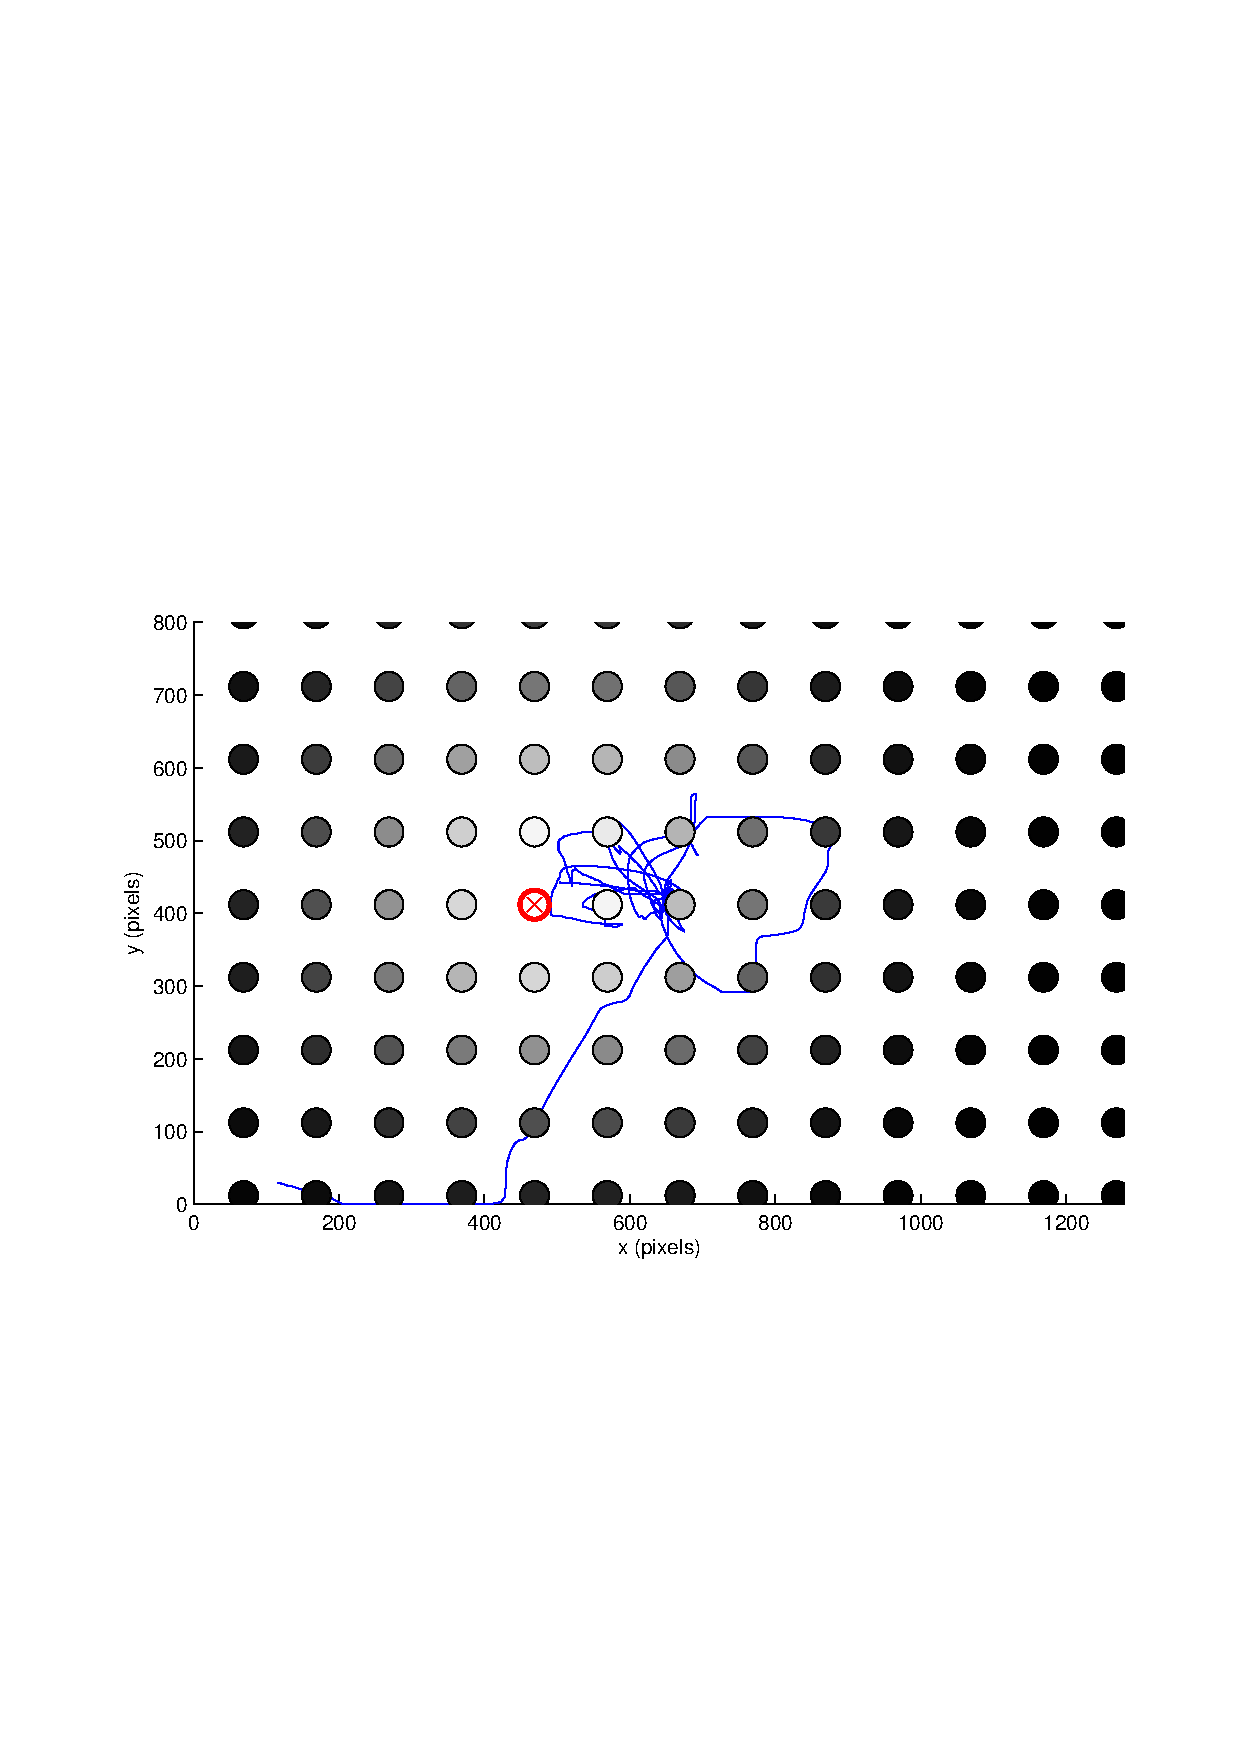
\includegraphics[width=0.9\textwidth]{MovieScreenshot.pdf}
\caption{A screen shot showing the cursor trace, the grid of phantom buttons and their probabilities. See text for details.}
\label{fig:CursorTracking}
\end{figure}

\cleardoublepage

\appendix
\chapter{Association proposals}
We begin with some useful identities. A Gaussian transition density model for a single target is given by

\begin{equation}
P(x_{t+1}|x_t) = \mathcal{N}(x_{t+1}|A x_t, Q).
\end{equation}

If the multiple step transition density is written as

\begin{equation}
P(x_{t+d}|x_t) = \mathcal{N}(x_{t+d}|A_d x_t, Q_d)
\end{equation}

then using standard identities we can write the recursion

\begin{IEEEeqnarray}{rCl}
P(x_{t+d+1}|x_{t}) & = & \int P(x_{t+d+1}|x_{t+d})P(x_{t+d}|x_t) dx_{t+d} \nonumber \\
 & = & \int \mathcal{N}(x_{t+d+1}|A x_{t+d}, Q) \mathcal{N}(x_{t+d}|A_d x_{t+d}, Q_d) dx_{t+d} \nonumber \\
 & = & \mathcal{N}(x_{t+d+1}|A \times A_d x_t, A Q_d A^T + Q).
\end{IEEEeqnarray}

Hence, by induction, we have

\begin{IEEEeqnarray}{rCl}
A_d & = & A^d \nonumber \\
Q_d & = & \sum_{k=0}^{d-1} (A^k) Q (A^k)^T.
\end{IEEEeqnarray}

Also, for $\lambda_t \ne 0$, and using the factorisation of equation~\ref{eq:MTFactorisedLikelihood}

\begin{IEEEeqnarray}{rCl}
P(y_{t+d}^{(\lambda_{t+d})}|x_{t}) & \propto & \int \mathcal{N}(y_{t+d}^{(\lambda_{t+d})}|C_{t+d} x_{t+d}, R) \mathcal{N}(x_{t+d}|A_d x_t, Q_d) dx_{t+d} \nonumber \\
                                   & = & \mathcal{N}(y_{t+d}^{(\lambda_{t+d})}|C_{t+d} A_d x_t, R_d)
\end{IEEEeqnarray}

where 

\begin{IEEEeqnarray}{rCl}
R_d & = & R + C_{t+d} Q_d C_{t+d}^T.
\end{IEEEeqnarray}

Here we derive an approximation for the `optimal' association proposal for a linear-Gaussian model. For nonlinear models, linear approximations may be used in the style of the EKF. The optimum form for the proposal distribution is given by

\begin{IEEEeqnarray}{rCl}
q(\lambda_{t-L+1:t}|x_{t-L}, Y_{t-L+1:t}) & & \nonumber \\
 & = & P(\lambda_{t-L+1:t}|x_{t-L}, Y_{t-L+1:t}) \nonumber \\
 & \propto & P(Y_{t-L+1:t}|\lambda_{t-L+1:t},x_{t-L}) P(\lambda_{t-L+1:t}|x_{t-L}) \nonumber \\
 & = & \prod_{\substack{k=1:L\\l=t-L+k}} P(Y_{l}|Y_{l+1:t} \lambda_{l:t}, x_{t-L}) P(\lambda_{l}).
\label{eq:AssPropSequential}
\end{IEEEeqnarray}

where the backward-predictive likelihood factors may be expanded as

\begin{equation}
P(Y_{l}|Y_{l+1:t} \lambda_{l:t}, x_{t-L}) = \int P(Y_{l}|x_{l}, \lambda_{l}) P(x_{l}|Y_{l+1:t}, \lambda_{l+1:t}, x_{t-L}) dx_{l}.
\label{eq:AssPropBackPredLike}
\end{equation}

We use the approximation

\begin{equation}
P(x_{l}|Y_{l+1:t}, \lambda_{l+1:t}, x_{t-L}) \approx P(x_{l}|Y_{l+d}, \lambda_{l+d}, x_{t-L})
\end{equation}

where $d$ is the minimum positive value such that $\lambda_{l+d} \ne 0$. This can be expanded as

\begin{IEEEeqnarray}{rCl}
\IEEEeqnarraymulticol{3}{l}{P(x_{l}|Y_{l+d}, \lambda_{l+d}, x_{t-L})} \nonumber \\
\qquad \qquad & \propto & \int P(Y_{l+d}|x_{l+d}, \lambda_{l+d}) P(x_{l+d}|x_{l}) dx_{l+d} P(x_{l}|x_{t-L}) \nonumber \\
 & \propto & \int \mathcal{N}(y_{l+d}^{(\lambda_{l+d})}|C x_{l+d}, R) \mathcal{N}(x_{l+d}|A_d x_{l}, Q_d) dx_{l+d} \mathcal{N}(x_{l}|A_k x_{t-L}, Q_k) \nonumber \\
 & \propto & \mathcal{N}(y_{l+d}^{(\lambda_{l+d})}|C_{l+d} A_d x_{l}, R + C_{l+d} Q_d C_{l+d}^T) \mathcal{N}(x_{l}|A_k x_{t-L}, Q_k) \nonumber .
\label{eq:AssPropStateExpansion}
\end{IEEEeqnarray}

Substituting equation~\ref{eq:AssPropStateExpansion} into equation~\ref{eq:AssPropBackPredLike}, we have

\begin{IEEEeqnarray}{rCl}
\IEEEeqnarraymulticol{3}{l}{P(Y_{l}|Y_{l+1:t} \lambda_{l:t}, x_{t-L})} \nonumber \\
\qquad & \stackrel{\sim}{\propto} & \int \mathcal{N}(y_{l}^{(\lambda_{l})}|C_{l} x_{l}, R) \mathcal{N}(y_{l+d}^{(\lambda_{l+d})}|C_{l+d} A_d x_{l}, R + C_{l+d} Q_d C_{l+d}^T) \mathcal{N}(x_{l}|A_k x_{t-L}, Q_k) dx_{l} \nonumber \\
 & \propto & \int \exp(-\frac{1}{2} \xi) dx_{l} \nonumber \\
 & \propto & \exp(-\frac{1}{2} \zeta).
\end{IEEEeqnarray}

The challenge now is to rearrange $\xi$ and hence find $\zeta$. Superscript $\lambda$s are omitted for clarity.

\begin{IEEEeqnarray}{rCl}
\xi & = & (y_{l} - C_{l} x_{l})^T R^{-1} (y_{l} - C_{l} x_{l}) \nonumber \\
    &   & + \: (y_{l+d} - C_{l+d} x_{l+d})^T R_d^{-1} (y_{l+d} - C_{l+d} x_{l+d}) \nonumber \\
    &   & + \: (x_{l} - A_k x_{t-L})^T Q_k^{-1} (x_{l} - A_k x_{t-L}) \nonumber \\
    & = & x_{l}^T \underbrace{[ C_{l}^T R^{-1} C_{l} + A_d^T C_{l+d}^T R_d^{-1} C_{l+d} A_d + Q_k^{-1} ]}_{\Sigma_{l}^{-1}} x_{l} \nonumber \\
    &   & - \: 2 \underbrace{[ y_{l}^T R^{-1} C_{l} + y_{l+d}^T R_d^{-1} C_{l+d} A_d + x_{t-L}^T A_k^T Q_k^{-1} ]}_{\mu_{l}^T \Sigma_{l}^{-1}} x_{l} \nonumber \\
    &   & + \: \underbrace{[ y_{l}^T R^{-1} y_{l} + y_{l+d}^T R_d^{-1} y_{l+d} + x_{t-L}^T A_k^T Q_k^{-1} A_k ]}_{C}
\end{IEEEeqnarray}

Carrying out the integral, an expression for $\zeta$ is now obtainable. Terms independent of $y_{l}$ are absorbed into the constant of proportionality, which is unimportant as it will cancel out during normalisation.

\begin{IEEEeqnarray}{rCl}
\zeta & = & C - \mu_{l}^T \Sigma_{l} \mu_{l} \nonumber \\
      & = & y_{l}^T \underbrace{[ I - R^{-1} C_{l} \Sigma C_{l} R^{-1} ]}_{S_{l}^{-1}} y_{l} \nonumber \\
      &   & - \: 2 \underbrace{[ y_{l+d}^T R_d^{-1} C_{l+d} A_d \Sigma_{l} C_{l}^T R^{-1} + x_{t-L}^T A_k^T Q_k^{-1} \Sigma_{l} C_{l}^T R^{-1} ]}_{m^T S^{-1}} y_{l} \nonumber \\
      &   & + \: \text{terms independent of $\zeta$}
\end{IEEEeqnarray}

Hence we arrive at the final expression

\begin{equation}
P(Y_{l}|Y_{l+1:t} \lambda_{l:t}, x_{t-L}) \propto \mathcal{N}(y_{l}^{(\lambda_{l})}|m_t, S_t).
\end{equation}

where

\begin{IEEEeqnarray}{rCl}
m_t      & = & S_t R^{-1} C_{l} \Sigma_{l} [ A_d^T C_{l}^T R_d^{-1} y_{l}^{(\lambda_{l})} + Q_k^{-1} A_k x_{t-L} ] \nonumber \\
S_t      & = & [ I - R^{-1} C_{l} \Sigma_{l} C_{l} R^{-1} ] \nonumber \\
\Sigma_t & = & [ C_{l}^T R^{-1} C_{l} + A_d^T C_{l+d}^T R_d^{-1} C_{l+d} A_d + Q_k^{-1} ]^{-1}
\end{IEEEeqnarray}

and as before

\begin{IEEEeqnarray}{rCl}
A_d & = & A^d \nonumber \\
Q_d & = & \sum_{k=0}^{d-1} (A^k) Q (A^k)^T \nonumber \\
R_d & = & R + C_{l+d} Q_d C_{l+d}^T .
\end{IEEEeqnarray}

We need a different expression for the case when $\lambda_{l+d} = 0$ for all $d = 1:t-l$. In this case, the future observations tell us nothing about the current state. Now the expression for the backward state prediction becomes

\begin{equation}
P(x_{l}|Y_{l+1:t}, \lambda_{l+1:t}, x_{t-L}) = P(x_{l}| x_{t-L})
\end{equation}

Proceeding as before, we have

\begin{IEEEeqnarray}{rCl}
P(Y_{l}|Y_{l+1:t} \lambda_{l:t}, x_{t-L}) &  & \nonumber \\
 & \propto & \int \mathcal{N}(y_{l}^{(\lambda_{l})}|C_{l} x_{l}, R) \mathcal{N}(x_{l}|A_k x_{t-L}, Q_k) dx_{l} \nonumber \\
 & = & \mathcal{N}(y_{l}^{(\lambda_{l})}|C_{l} A_k x_{t-L}, R_k).
\end{IEEEeqnarray}

Finally, in the special case where $\lambda_{l} = 0$,

\begin{equation}
P(Y_{l}|Y_{l+1:t} \lambda_{l:t}, x_{t-L}) \propto V^{-1}.
\end{equation}


\bibliographystyle{dcu}%_noURLs}
\bibliography{D:/pb404/Bibtex/OTbib}


\end{document}